\documentclass{beamer}
%\documentclass[handout]{beamer}

\usepackage{etex}
\usepackage[utf8]{inputenc}
\usepackage[T1]{fontenc}
\usepackage[english]{babel}
\usepackage{color}
\usepackage{colortbl}
\usepackage{amsmath}
\usepackage{amsfonts}
\usepackage{amssymb}
\usepackage{textcomp}
\usepackage{natbib}
\usepackage{multirow}
\usepackage{nicefrac}
\usepackage{multicol}
\usepackage{url}
\usepackage{gb4e-}
\usepackage{pifont}
\usepackage{bbding}
\usepackage{tree-dvips}

\title[Working with Web Corpora]{\Large Working with Web Corpora}
\author[Felix Bildhauer and Roland Schäfer]{\Large Felix Bildhauer, Roland Schäfer}
\institute{IDS Mannheim, FU Berlin}
\date{GaC 2016 pre-conference tutorial, \today}

\usetheme{FUBerlin}
\definecolor{beamer@fuorange}{rgb}{.8,.3,0}
\definecolor{Gray}{gray}{0.5}
\definecolor{Black}{gray}{0}
\definecolor{Orinj}{rgb}{0.9,0.4,0.1}
\definecolor{Greene}{rgb}{0,0.5,0}
\setbeamercolor{alerted text}{fg=Orinj}
\newcommand{\orinj}[1]{\textcolor{Orinj}{#1}}
\newcommand{\greene}[1]{\textcolor{Greene}{#1}}
\newcommand{\graw}[1]{{\color[rgb]{0.5,0.5,0.5}#1}}
\newcommand{\blaw}[1]{{\color[rgb]{0.2,0.2,0.9}#1}}
\newcommand{\grien}[1]{{\color[rgb]{0.1,0.6,0.1}#1}}
\newcommand{\myalert}[2]{{\color<#1>[rgb]{0,0.7,0}#2}}
\newcommand{\eg}{e.\,g.}
\newcommand{\Eg}{E.\,g.}
\newcommand{\ie}{i.\,e.}
\newcommand{\Ie}{I.\,e.}
\newcommand{\Dim}{\cellcolor{Gray}}
\newcommand{\Off}{\cellcolor{Black}}

\titlegraphic{}
\fuberlinlogon{0.8cm}
\renewcommand{\fuberlinfootstring}{\insertshortauthor{} \number\year, \insertshortinstitute}

\setcounter{tocdepth}{1}

%\AtBeginSection[]
%{
%  \begin{frame}
%    \frametitle{We are here\dots}
%      \begin{multicols}{2}
%         \footnotesize
%         \tableofcontents[currentsection]
%      \end{multicols}
%   \end{frame}
%}

\newcommand{\xxx}{\hspaceThis{[}}
\newcommand{\Lf}{
  \setlength{\itemsep}{1pt}
  \setlength{\parskip}{0pt}
  \setlength{\parsep}{0pt}
}

\newcounter{lastpagemainpart}

\begin{document}

\fuberlintitlepage


\section{Webcorpora 2005--2015}


\subsection{First generation}

\begin{frame}
	{First generation: WaCky and early WAC workshops}
	\begin{itemize}
  		\item original goal: BNC for free
  		\item not much methodological discussion from linguistic pov
  		\item WaCky: no meta data, destructive normalization\\minimal linguistic annotation
  		\item COW11 and COW12: similar to WaCky
  		
  		\vspace{0.5cm}
  			
  		\item When we started: fragmented WAC scene already\\monetization of web corpora (SketchEngine, BYU)
	\end{itemize}
\end{frame}

\begin{frame}
	{Second generation?}
	\begin{itemize}
	  \item DeRiK: \alert{miniature corpora}, manual construction like DWDS-KK
	  \item SketchEngine\slash Lexical Computing: technologically innovative,\\made for lexicographers, \alert{expensive}
	  \item Glowbe von BYU: questionable in many ways, \alert{expensive}
	\end{itemize}
\end{frame}

\begin{frame}
	{What's unique about COW and COCO?}
	\begin{itemize}
	  \item technologically most advanced\\(cleanup, normalization, linguistic annotation, meta data)
	  \item no narrow optimization for lexicography
	  \item \alert{very large}: variation in non-standard\slash rare phenomena
	  \item \alert{free}, only limited by German IP laws
	  
	  \vspace{0.5cm}
	   
	  \item \alert{COW is the only remaining web corpus project\\which is technologically state of the art,\\creating free and large corpora.}
	\end{itemize}
\end{frame}

%\subsection{Rechtslage}
%
%\begin{frame}
%	{Das deutsche Urherberrecht}
%	\begin{itemize}
%	  \item umfassender Schutz des Werkes vor jeglicher Verwendung,\\der der Autor nicht zugestimmt hat
%	  \item anders als viele denken: Art der Verwendung\\(kommerziell vs.\ Wissenschaft) spielt \alert{keine Rolle}
%	  \item für jeden Text explizite Erlaubnis erforderlich
%	  \item verwaiste Werke nicht automatisch frei, erheblicher Aufwand beim Auffinden des Urhebers muss nachgewiesen werden
%	  \item gemacht für Bücher und Opern -- pervers für Blogs, Foren\\oder von Spiegel Online mit Rechtschreibfehlern versehene DPA-Meldungen  
%	\end{itemize}
%\end{frame}
%
%\begin{frame}
%	{Lösung}
%	\begin{itemize}
%		\item langfristig: Ausnahmeregelungen für Wissenschaft
%		\item Fair Use gilt als inkompatibel zu deutschem Urheberrecht
%		\item also \alert{vollständige Reform}, einschließlich Verwertungsgesellschaften 
%		\item ohne Lobbyarbeit und Allianzen mit anderen Disziplinen\\keine Chance für Korpuslinguitik
%		\item Initiative aus GSCL AK DigHum und ACL SIGWAC:\\erste Podiumsduskussion bei WAC-X @ ACL 2016\\12.\ August in Berlin
%		\item Alternative: Unterwanderung, s. COCO
%	\end{itemize}
%\end{frame}
%


\section{Web corpus construction}

\subsection{Why use web corpora?}

\begin{frame}
  {Why corpora from the web?}

  \begin{itemize}
  \item \alert{Size}: alleviates data sparseness problems with rare phenomena
  \item \alert{Content}: registers not found in traditional corpora\\ (forum discussions, blogs, fan-fiction etc.)
  \item \alert{Replicability}: research with static corpus\\
    vs.\ research based on search engine results
  \item \alert{Availability}: data can be locally processed with preferred tools.
  \item \alert{Cost}: (virtually) free
  \end{itemize}
\end{frame}


\begin{frame}
  {Some potential drawbacks of web corpora}

  \begin{itemize}
  \item \alert{Noise}: from properties of web documents\\
    and from imperfect processing
  \item \alert{Meta data} (of the kind linguists are interested in):\\
    not encoded in web documents in a reliable way
  %   \begin{itemize}
%     \item no stratification by registers and/or text types
%     \item either manual classification (unrealistic for very large corpora)
%     \item or automatic classification, based on easy-to-compute features
%     \end{itemize}
  \end{itemize}
\end{frame}


\subsection{Web corpus construction: Overview}

\begin{frame}{Web corpus construction: workflow}

\scalebox{.7}{
  \begin{tabular}{c}
    \fbox{\alert<2->{Data collection}}\\[.6ex]
$\Downarrow$\\[.6ex]
    \fbox{Removal of markup, scripts etc. }\\[.6ex]
$\Downarrow$\\[.6ex]
    \fbox{\alert<2->{Detection/removal of ``boilerplate''}}\\[.6ex]
$\Downarrow$\\[.6ex]
    \fbox{\alert<2->{Detection/removal of ``non-texts''}}\\[.6ex]
$\Downarrow$\\[.6ex]
    \fbox{\alert<2->{Detection/removal of (near-) duplicates}}\\[.6ex]
$\Downarrow$\\[.6ex]
    \fbox{\alert<2->{Linguistic post-processing}}
  \end{tabular}
}

\vspace{.5cm}
 \onslide<2->{
These steps involve design decisions\\
which affect the properties of the final corpus.}
\end{frame}


\begin{frame}{Workflow II}
  \begin{columns}
    \begin{column}{5cm}
    \scalebox{.7}{
\begin{tabular}{c}

\fbox{\alert<1>{Data collection}}\\[.6ex]
$\Downarrow$\\[.6ex]
    \fbox{Removal of markup, scripts etc. }\\[.6ex]
$\Downarrow$\\[.6ex]
    \fbox{\alert<2>{Detection/removal of ``boilerplate''}}\\[.6ex]
$\Downarrow$\\[.6ex]
    \fbox{\alert<3>{Detection/removal of ``non-texts''}}\\[.6ex]
$\Downarrow$\\[.6ex]
    \fbox{\alert<4>{Detection/removal of (near-) duplicates}}\\[.6ex]
$\Downarrow$\\[.6ex]
    \fbox{\alert<5->{Linguistic post-processing}}
\end{tabular}
}
    \end{column}

    \begin{column}{5cm}
      \begin{itemize}
      \item Which sampling procedure/crawling strategy?
      \item<2-> What should count as ``boilerplate''?
      \item<3-> Which documents contribute ``good text''?
      \item<4-> Which amount of duplication is acceptable?
      \item<5-> How do we treat non-standard orthography, spelling errors, non-words etc.?
      \end{itemize}
    \end{column}
  \end{columns}
\end{frame}



%\subsection{Data collection}
%
%%\subsection{The Web (Graph)}
%
%\begin{frame}
%  {Links}
%  \begin{itemize}
%    \item The web consists of pages and links between them.
%    \item Each page has an \alert{in-degree} (no.\ of links to that page),
%    \item and an \alert{out-degree} (no.\ of links on that page).
%  %  \item The in-degree of pages is distributed by a \alert{power law}\\
%  %    ($\frac{1}{a^{2.1}}$ according to \citealp[][426]{Manning-ea2009}.)
%    \item Pages with a higher in-degree are easier to find, but not necessarily the more interesting ones for corpus construction.
%  \end{itemize}
%\end{frame}
%
%\begin{frame}
%  {The structure of the web}
%  \begin{center}
%    
\includegraphics[width=6cm]{graphicswcc/bowtie}\\
%    
%    \vspace{0.5cm}
%    \footnotesize\cite[427]{Manning-ea2009}\\
%    Contrary to common intuition, \citealp{Broder-ea00} found that the IN, OUT, SCC, and TENDRIL components are not extremely different in size.\\
%    A more detailed report on the sizes: \cite{Serrano-ea2007}.
%  \end{center}
%\end{frame}
%
%\begin{frame}
%  {Inaccessible web content (deep web)}
%  \begin{itemize}
%    \item explicitly \alert{hidden} from spiders\\
%      (Robots Exclusion, intentional fooling\slash spoofing)
%    \item requiring \alert{login}\\
%      (social networks, some forums, intranet gateways)
%    \item \alert{in-degree$=0$}
%    \item \graw{in-degree$>0$, but \alert{too far away} from any seed URL\\
%    (which are mostly search-engine indexed pages;\\
%  depends on crawling strategy)}
%  \end{itemize}
%\end{frame}
%
%\begin{frame}
%  {Static and dynamic web content}
%  \begin{itemize}
%    \item By definition, \alert{static web content} is any page which is\\
%      not generated by a database\slash content generation system,\\
%      but edited manually.
%    \item Today, most content is \alert{dynamic} (CMS, blogs, etc.),\\
%      and the static\slash dynamic distinction should not play\\
%      a great role in crawling for corpus construction.
%    \item The problem is rather the separation of (static or dynamic) \alert{linguistically relevant} from \alert{irrelevant} content\\
%      (time tables, product listings, etc.).
%  \end{itemize}
%\end{frame}
%
%\begin{frame}
%  {Top-level domains and national dialects}
%  \begin{itemize}
%    \item It is common practice to crawl national TLDs for content\\
%      in the corresponding national language.
%    \item \cite{Cook-Hirst2012} conclude that the TLDs for \texttt{.ca}\\
%      and \texttt{.uk} indeed \alert{represent national variants} of English.
%   % \item Methods used: \alert{keyword} comparison with existing corpora \citep{Kilgarriff2009}, \alert{spelling variants}.
%    \item Problems with TLD crawls:
%      \begin{itemize}
%	\item In some countries, \texttt{.com} has a high prestige:\\
%	  \url{http://elpais.com}, \url{http://www.lavanguardia.com/}, \url{http://www.marca.com/}
%	\item TLDs of countries with more than one official language\\
%	  (\eg, Indonesia, Spain) yield relatively fewer results\\
%	  in the target language.
%      \end{itemize}
%   \end{itemize}
%\end{frame}
%
%
%
%\begin{frame}{Breadth-first crawling}
%
%Common practice (e.\,g.\ WaCky, COW): follow \textbf{all} links on a page\\[2ex]
%
%Pro:
%
%  \begin{itemize}
%  \item effective: yields lots of data whithin a short time
%  \item open source software available 
%  \end{itemize}
%
%Con:
%
%\begin{itemize}
%\item very susceptible to page rank: no uniform random sample
%\item unknown sampling bias
%\end{itemize}
%  
%\end{frame}
%
%
%\begin{frame}
%  {Alternative: Random walks}
%
%Yet not used for web corpora: follow \textbf{one} link on a page
%
%Pro:
%
%\begin{itemize}
%\item known sampling bias: can be corrected for
%\item uniform random sample of web documents
%\end{itemize}
%
%Con:
%
%\begin{itemize}
%\item much less effective than BF
%\item probably not suitable for giga-token corpora
%\end{itemize}
%
%\end{frame}





\subsection{Boilerplate detection}

\begin{frame}
  {Boilerplate detection}

Boilerplate is text accompanying the main text on a web page:

\begin{itemize}
\item navigation bars
\item banners
\item advertisements
\item other layout elements 
\item copyright notes
\end{itemize}

\pause

Boilerplate is typically not text produced by person on a particular occasion, but rather

\begin{itemize}
\item generated by content management systems
\item similar or identical on many web pages of the same website
\item similar or identical across web sites 
\end{itemize}
\end{frame}


\begin{frame}
  {Why detect boilerplate?}

Boilerplate elements bias the frequency of linguistic items in the final corpus.

\begin{itemize}
\item One of the most frequent tokens in an experimental German web corpus: \textit{mehr} `more', as in \textit{read more\ldots}\\[1ex] \pause
\item One of the most frequent sentences in an experimental English web corpus: \textit{You are not allowed to post new content in the forum.}
\end{itemize}
\end{frame}


\begin{frame}
  {Text}
  \begin{center}
    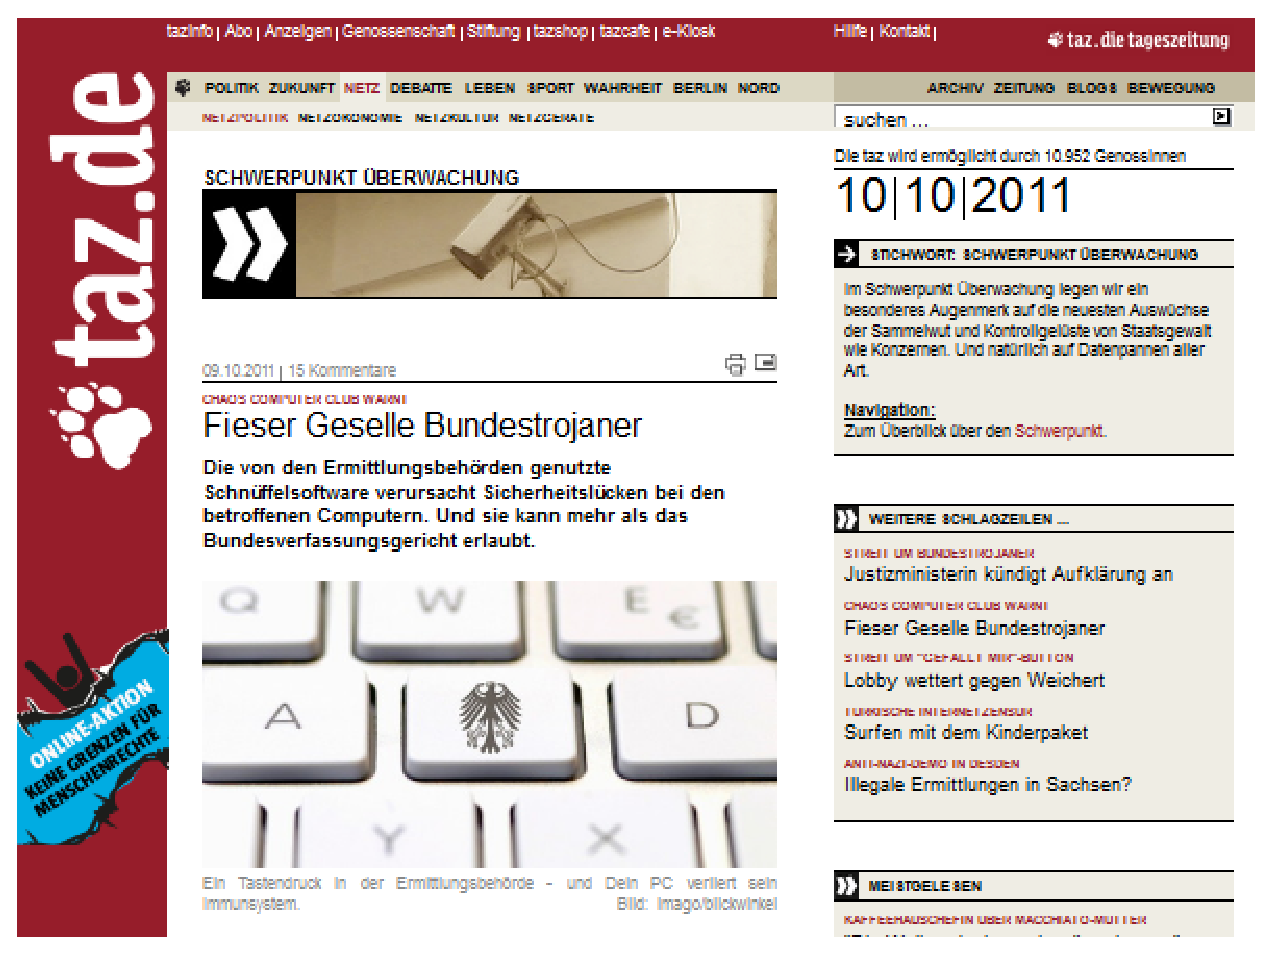
\includegraphics[width=8cm]{graphicswcc/webseite}
  \end{center}
\end{frame}

\begin{frame}
  {Text (II)}
  \begin{center}
    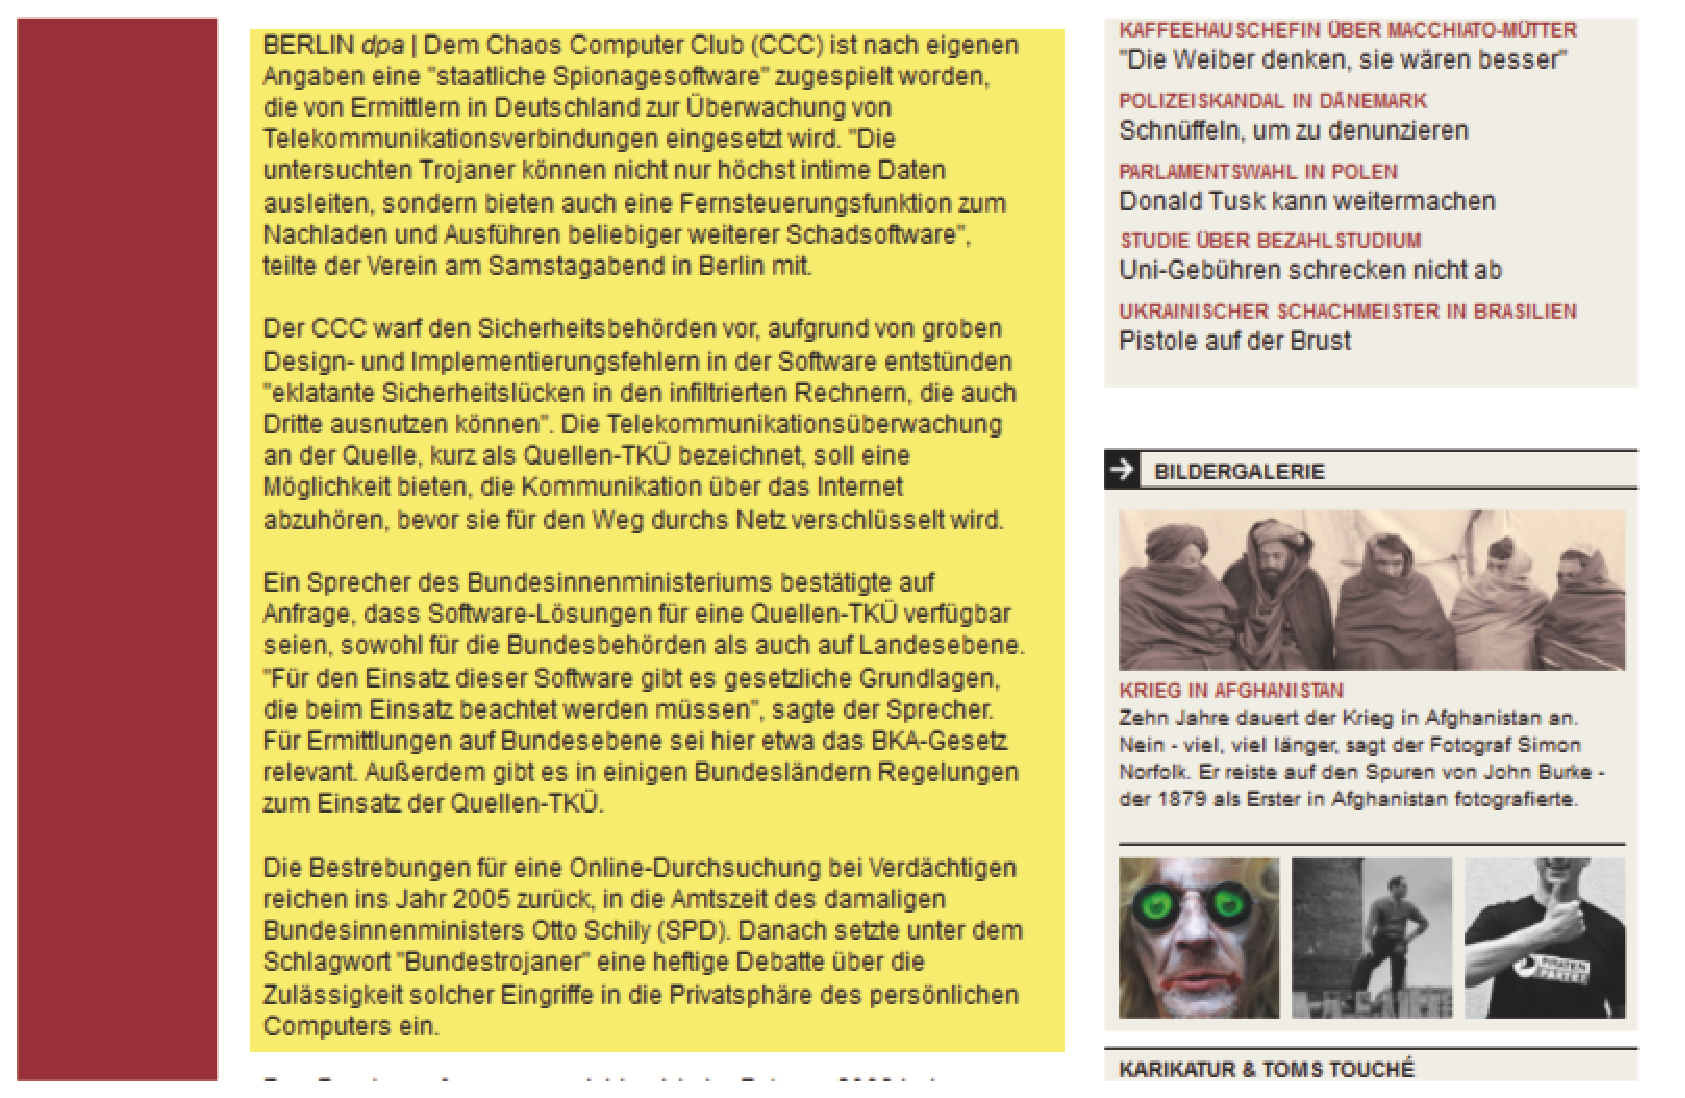
\includegraphics[width=8cm]{graphicswcc/webseite2}
  \end{center}
\end{frame}

\begin{frame}
  {Text (III)}
  \begin{center}
    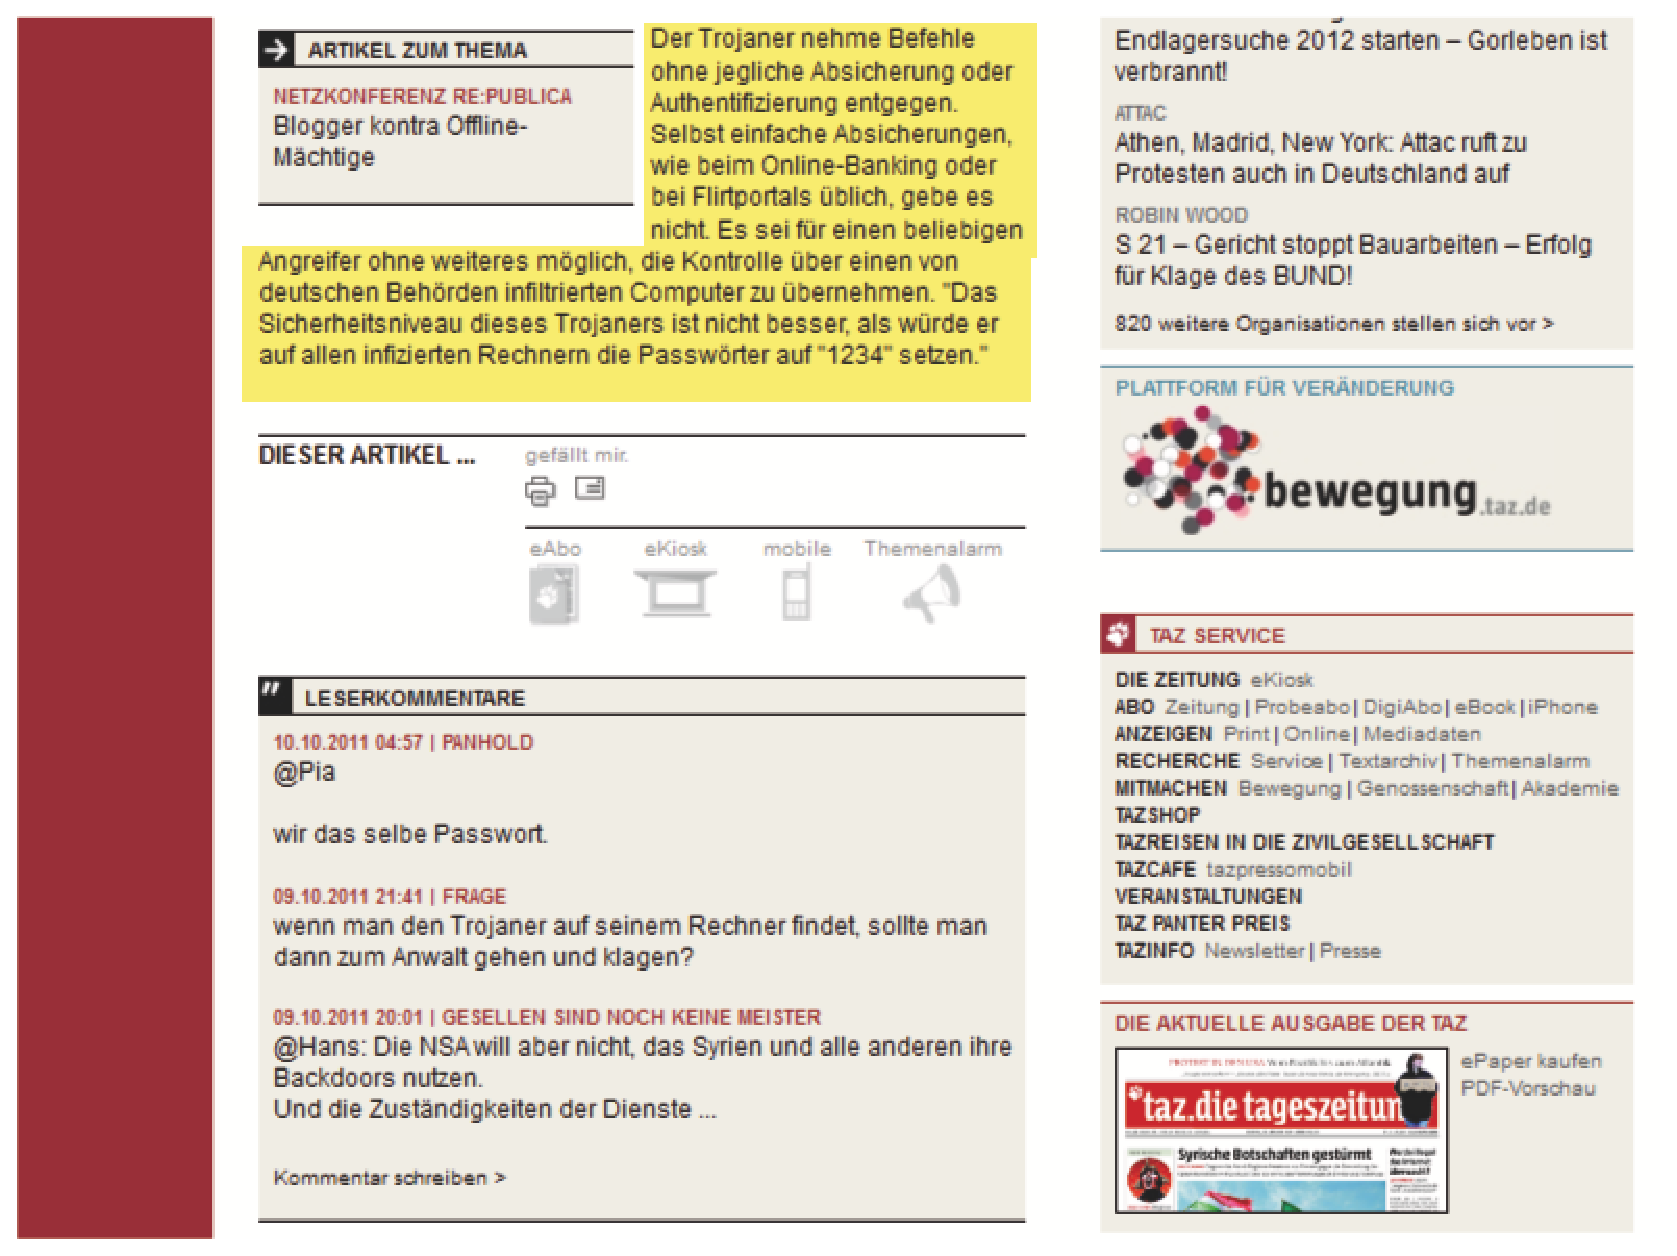
\includegraphics[width=8cm]{graphicswcc/webseite3}
  \end{center}
\end{frame}




\begin{frame}
  {What should count as boilerplate? }
  \begin{center}
    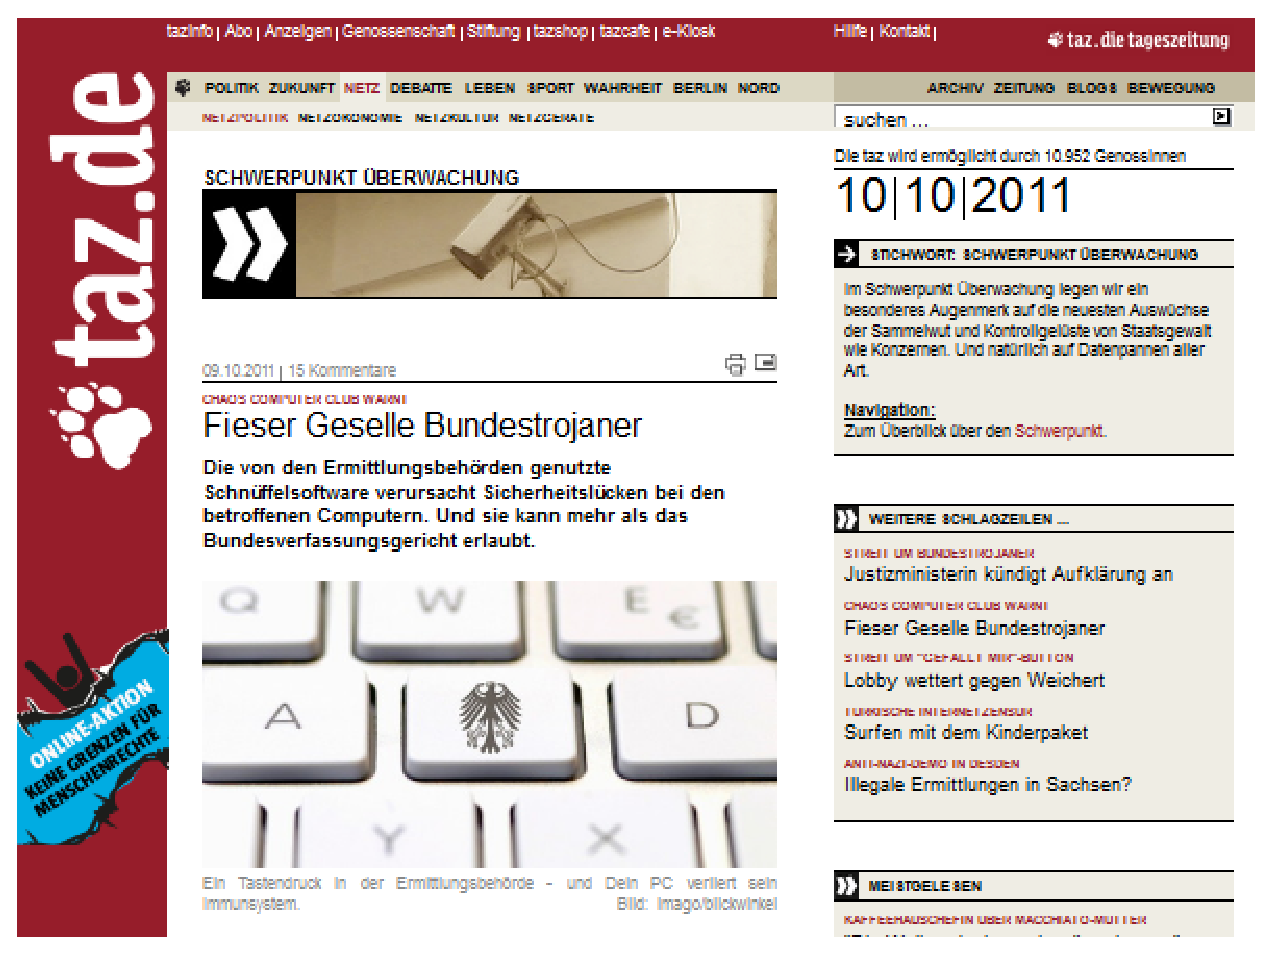
\includegraphics[width=8cm]{graphicswcc/webseite}
  \end{center}
\end{frame}

\begin{frame}
  {What should count as boilerplate? (II)}
  \begin{center}
    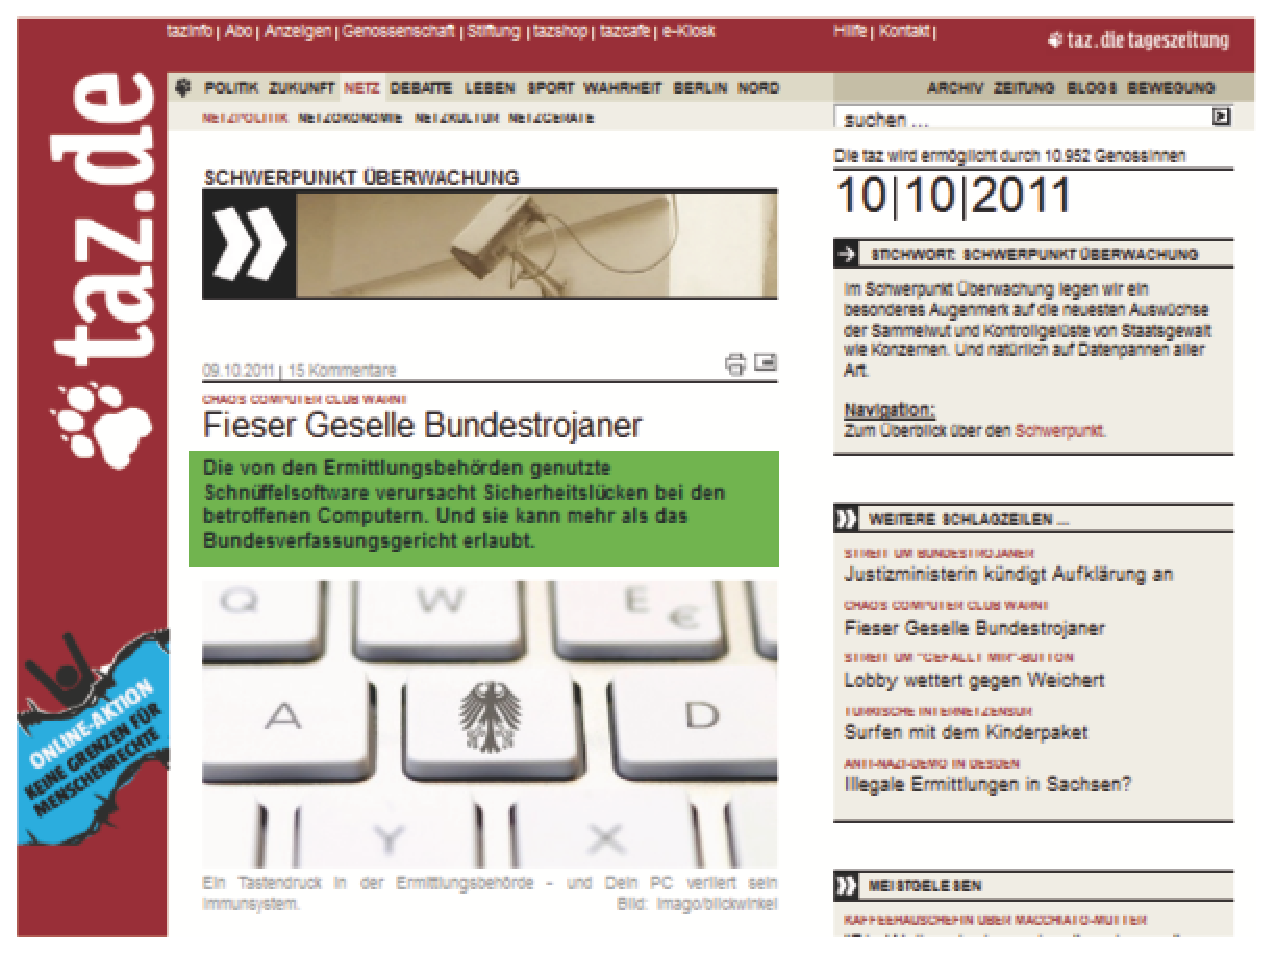
\includegraphics[width=8cm]{graphicswcc/webseite-b}
  \end{center}
\end{frame}


\begin{frame}
  {What should count as boilerplate? (III)}
  \begin{center}
    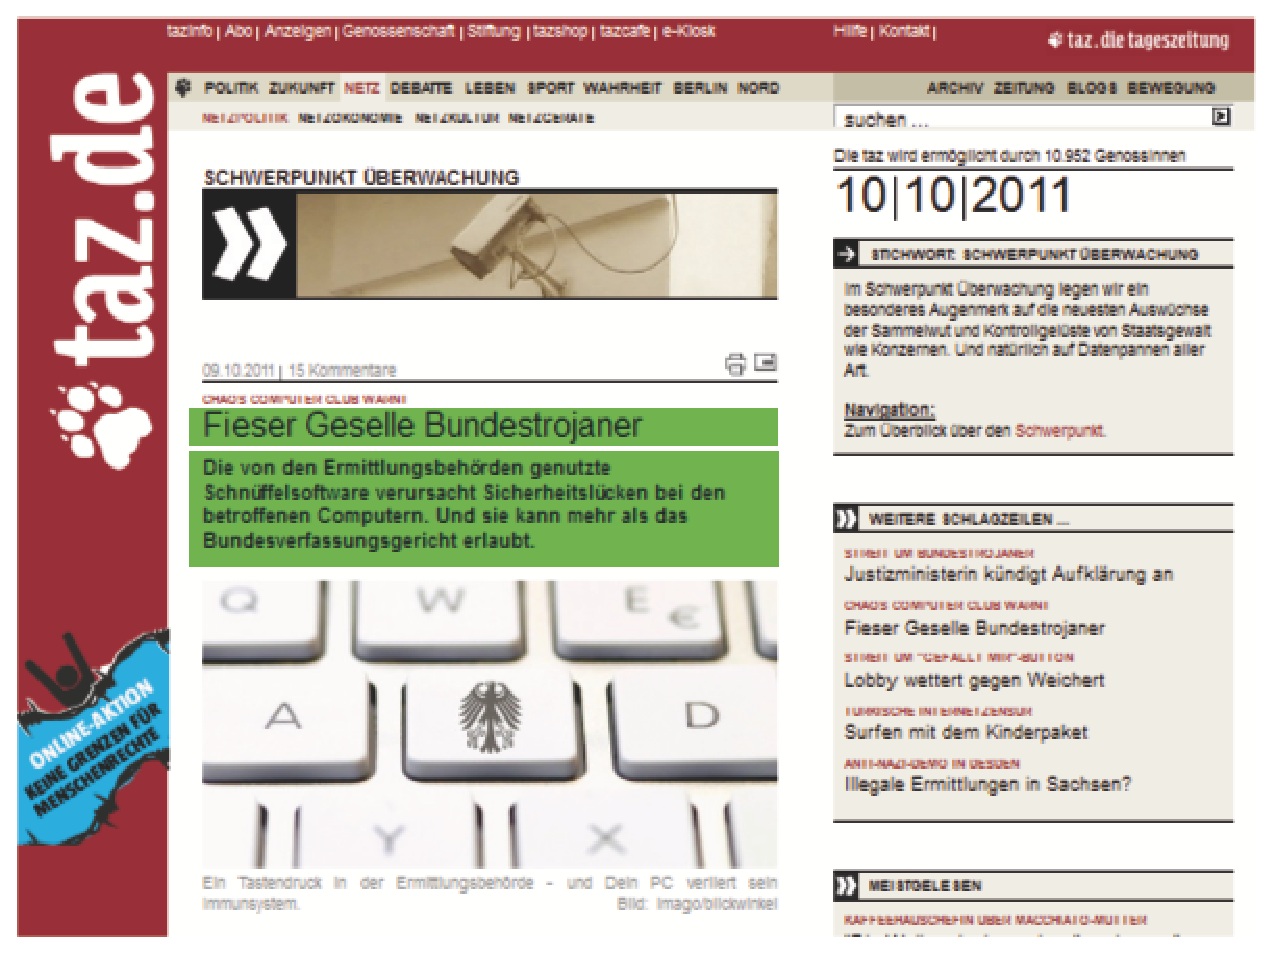
\includegraphics[width=8cm]{graphicswcc/webseite-c}
  \end{center}
\end{frame}



\begin{frame}
  {What should count as boilerplate? (IV)}
  \begin{center}
    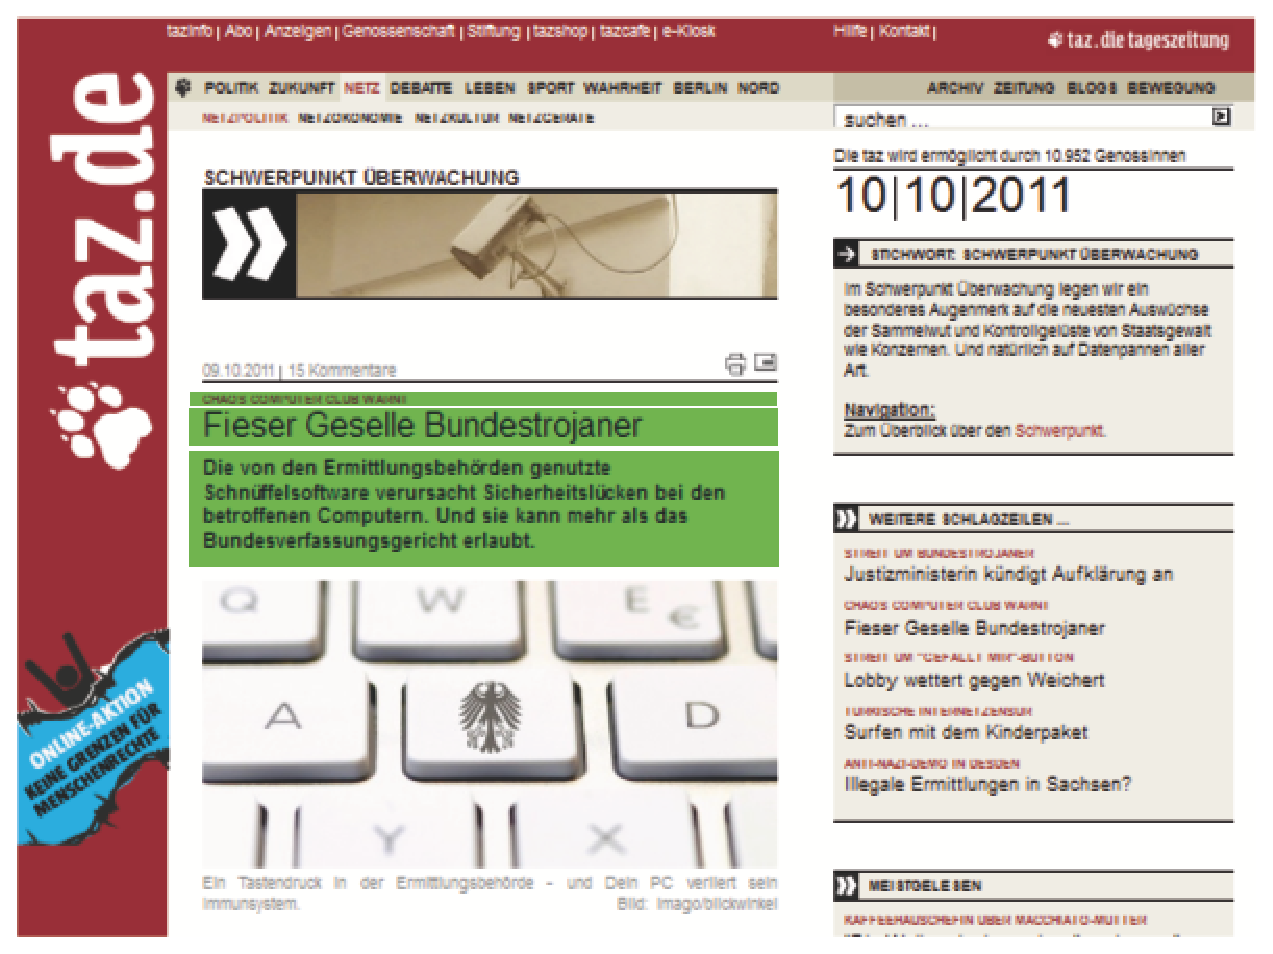
\includegraphics[width=8cm]{graphicswcc/webseite-d}
  \end{center}
\end{frame}


\begin{frame}
  {What should count as boilerplate? (V)}
  \begin{center}
    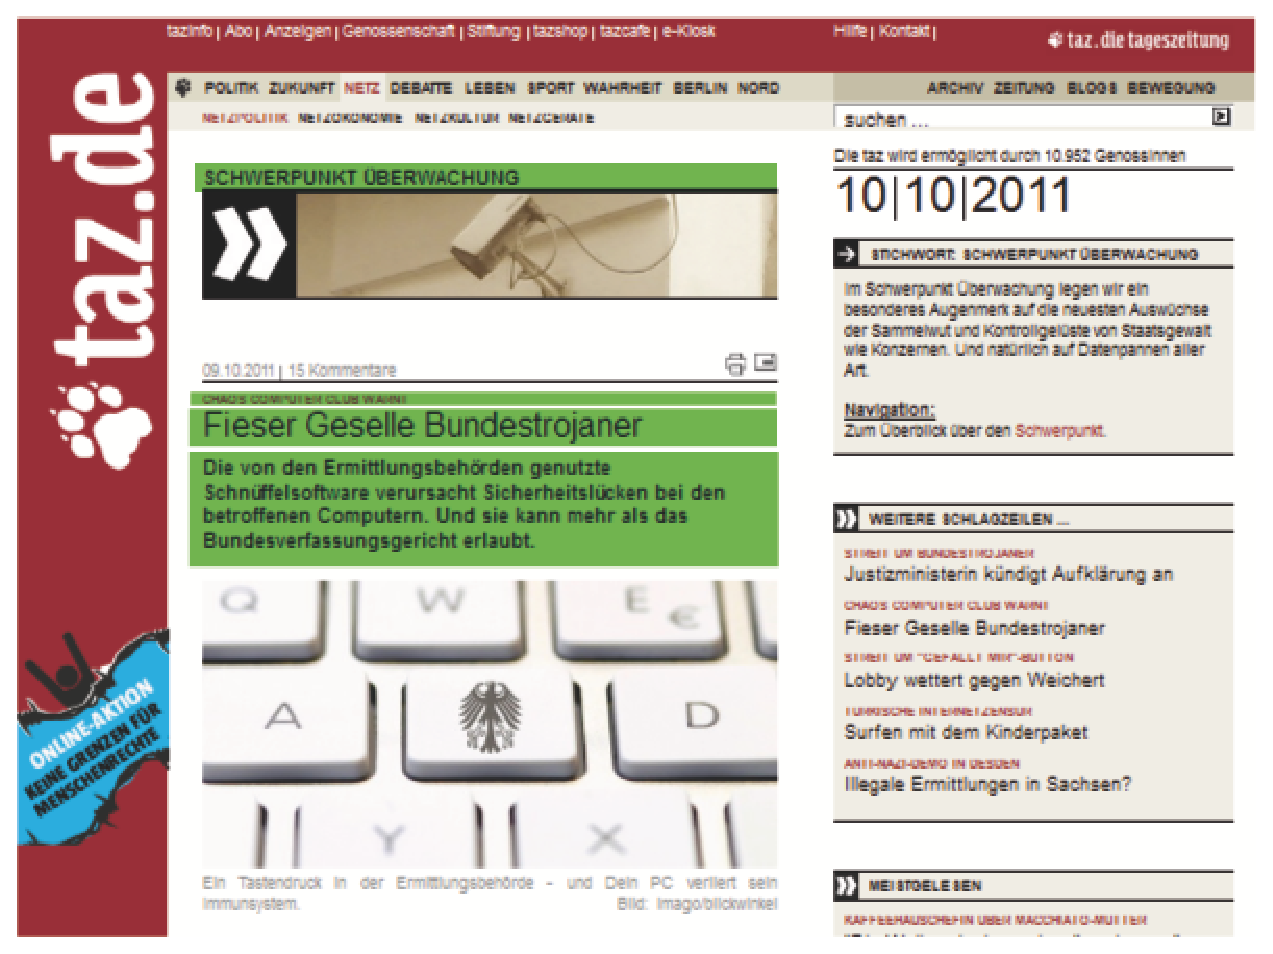
\includegraphics[width=8cm]{graphicswcc/webseite-e}
  \end{center}
\end{frame}



\begin{frame}
  {What should count as boilerplate?(VI)}
  \begin{center}
    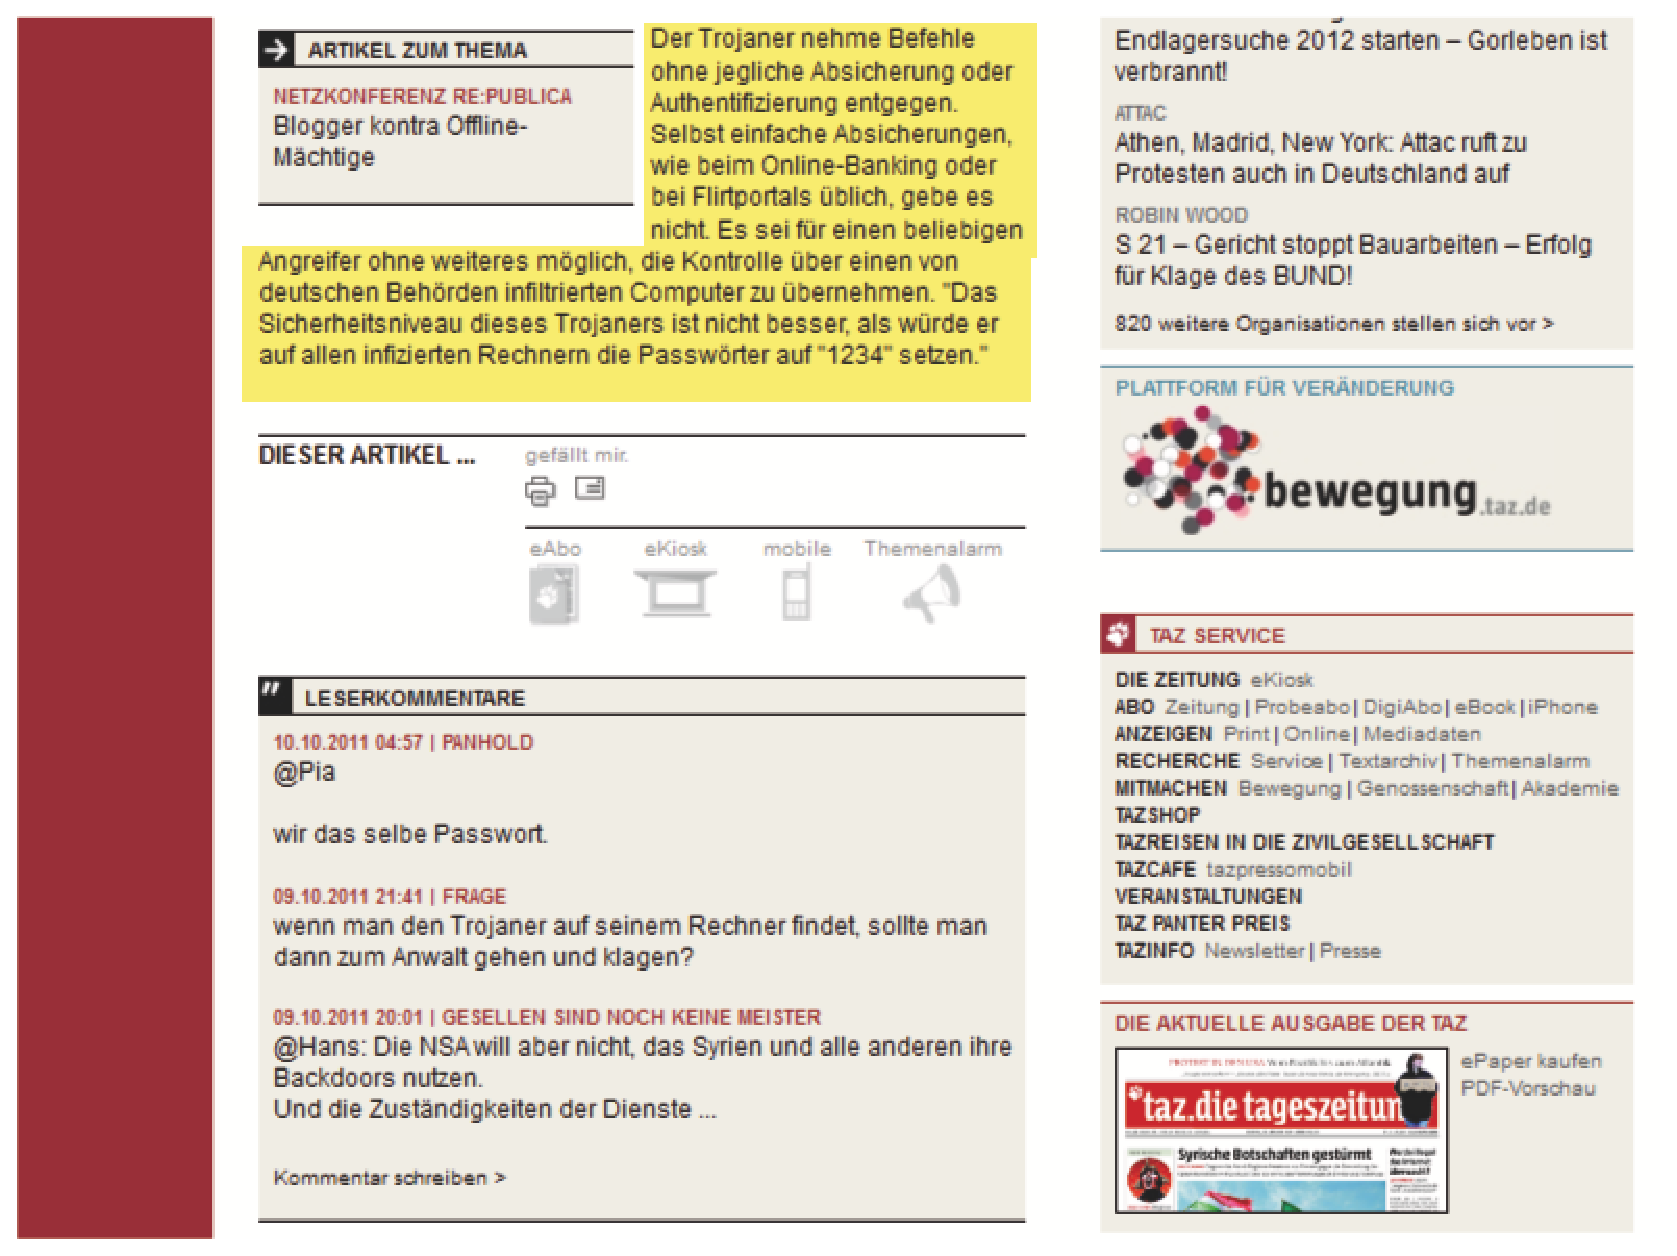
\includegraphics[width=8cm]{graphicswcc/webseite3}
  \end{center}
\end{frame}


\begin{frame}
  {What should count as boilerplate? (VII)}
  \begin{center}
    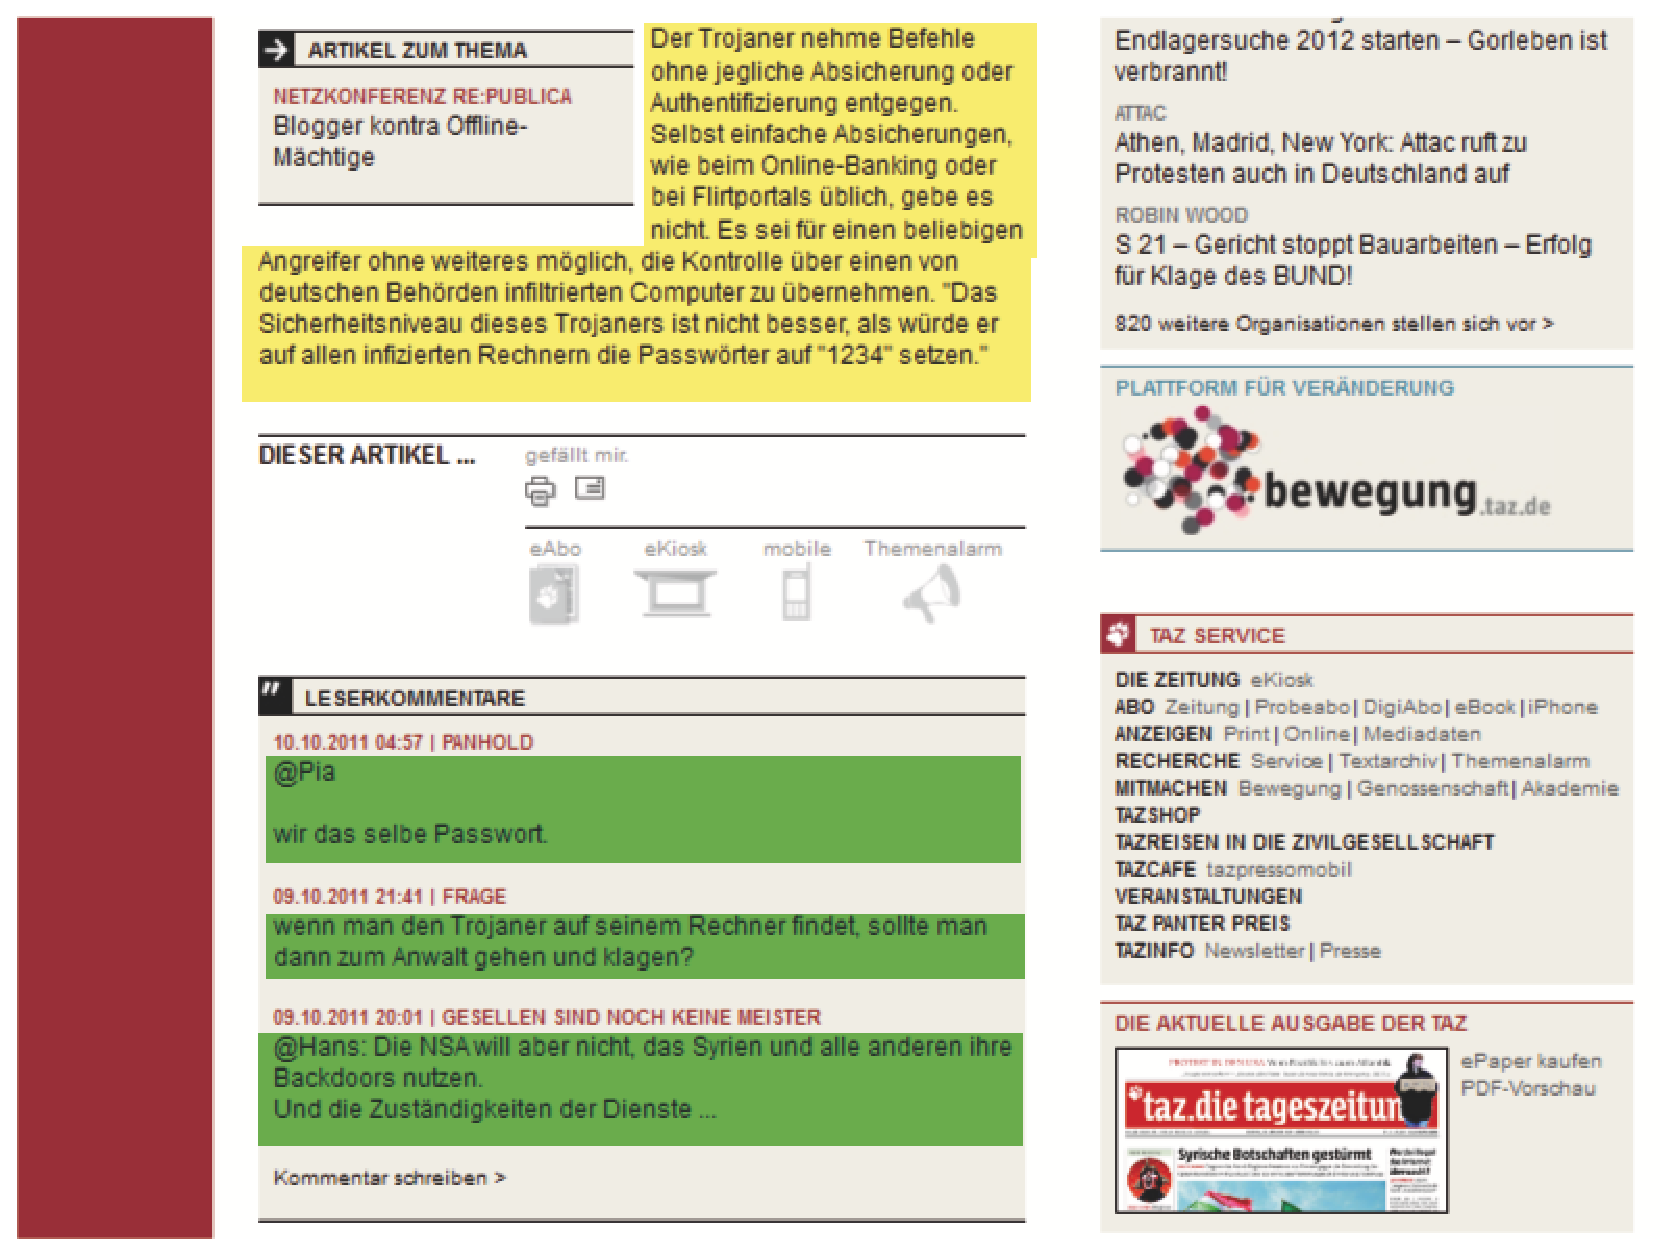
\includegraphics[width=8cm]{graphicswcc/webseite3-b}
  \end{center}
\end{frame}


\begin{frame}
  {What should count as boilerplate? (VIII)}
  \begin{center}
    \includegraphics[width=8cm]{graphicswcc/webseite3-c}
  \end{center}
\end{frame}


\begin{frame}
  {What should count as boilerplate?  (IX)}
  \begin{center}
    \includegraphics[width=8cm]{graphicswcc/webseite3-d}
  \end{center}
\end{frame}


\begin{frame}
  {What should count as boilerplate? (X)}
  \begin{center}
    \includegraphics[width=8cm]{graphicswcc/webseite3-e}
  \end{center}
\end{frame}


\begin{frame}
{Automatic detection of boilerplate}

Boilerplate must be detected automatically.\\[2ex] %, given   Typical web corpora contain millions of documents:

Machine learning techniques:
\begin{itemize}
\item Manually annotate a number of paragraphs: boilerplate yes/no
\item Calculate a number of features from each paragraph
  \begin{itemize}
  \item e.\,g., number of text characters, number of HTML tags, position in HTML-document
  \end{itemize}
\item Train a classifier to reproduce the human's decisions 
  \begin{itemize}
  \item we use an artificial neural network (multilayer perceptron)
  \end{itemize}
\end{itemize}
\end{frame}


% \begin{frame}
%   {Overview of the boilerplate removal scene}
%   \begin{itemize}
%     \item Most prominently, the \alert{CLEANEVAL} competition \citep{Baroni-ea2008} produced a variety of efforts in boilerplate removal and document structure recognition:
%       \begin{itemize}
% 	\item \cite{Bauer-ea2007}, \cite{Evert2007}, \cite{Weizheng-Abou2007}, \cite{Girardi2007}, \cite{Hoffman-Weerkamp2007}, \cite{Issac2007}, \cite{Marek-ea2007}, \cite{Saralegi-Leturia2007}
%       \end{itemize}
%     \item Furthermore, the WaCky corpora have undergone some boilerplate removal method \citep{Baroni-ea2009}.
%     \item Claiming to have achieved a very high accuracy: \cite{Spousta2008}, based on \cite{Marek-ea2007}.
%     \item You can also check out JustText at \url{http://nlp.fi.muni.cz/projekty/justext/} online, based on \cite{Pomikalek2011}.
%   \end{itemize}
% \end{frame}


\begin{frame}
{Automatic detection of boilerplate (II)}

Automatic detection is not perfect:

\begin{itemize}
\item some boilerplate will not be discovered (recall $<1$)
\item some paragraphs will be mistakenly classified as boilerplate (precision $<1$)
\end{itemize}

Keep this in mind when working with web corpora,\\
and double check any implausible frequency figures.
  
\end{frame}



\begin{frame}{Boilerplate: removal vs.\ flagging}
  
``Classic'' approach (e.\,g., WaCky, COW2012): remove boilerplate.

  \begin{itemize}
  \item Alternative: do not remove, but flag\\
    (possibly with a confidence score)
    \item \alert{Pro} -- User do not have to rely on:
      \begin{itemize}
      \item the corpus designer's definition of boilerplate
      \item the performance of an automatic classifier
      \end{itemize}
\pause
    \item \alert{Con}:
      \begin{itemize}
      \item increase in corpus size
%      \item depending on querying architecture: 
      \end{itemize}
  \end{itemize}
\end{frame}


\subsection{Document filtering}


\begin{frame}
{Document filtering}

Ideally, the final corpus should contain only ``good'' documents.

``Good'':

\begin{itemize}
\item only documents in the target language
\item documents containing predominantly text\\
  (i.\,e., coherent and connected text)
\end{itemize}

\pause

This excludes certain document types:

\begin{itemize}
\item lists (e.\,g.\ company names, vocabulary items)
\item tag clouds
\item etc.
\end{itemize}

\end{frame}



\begin{frame}{Example: a ``good'' document}
  
  \begin{center}
     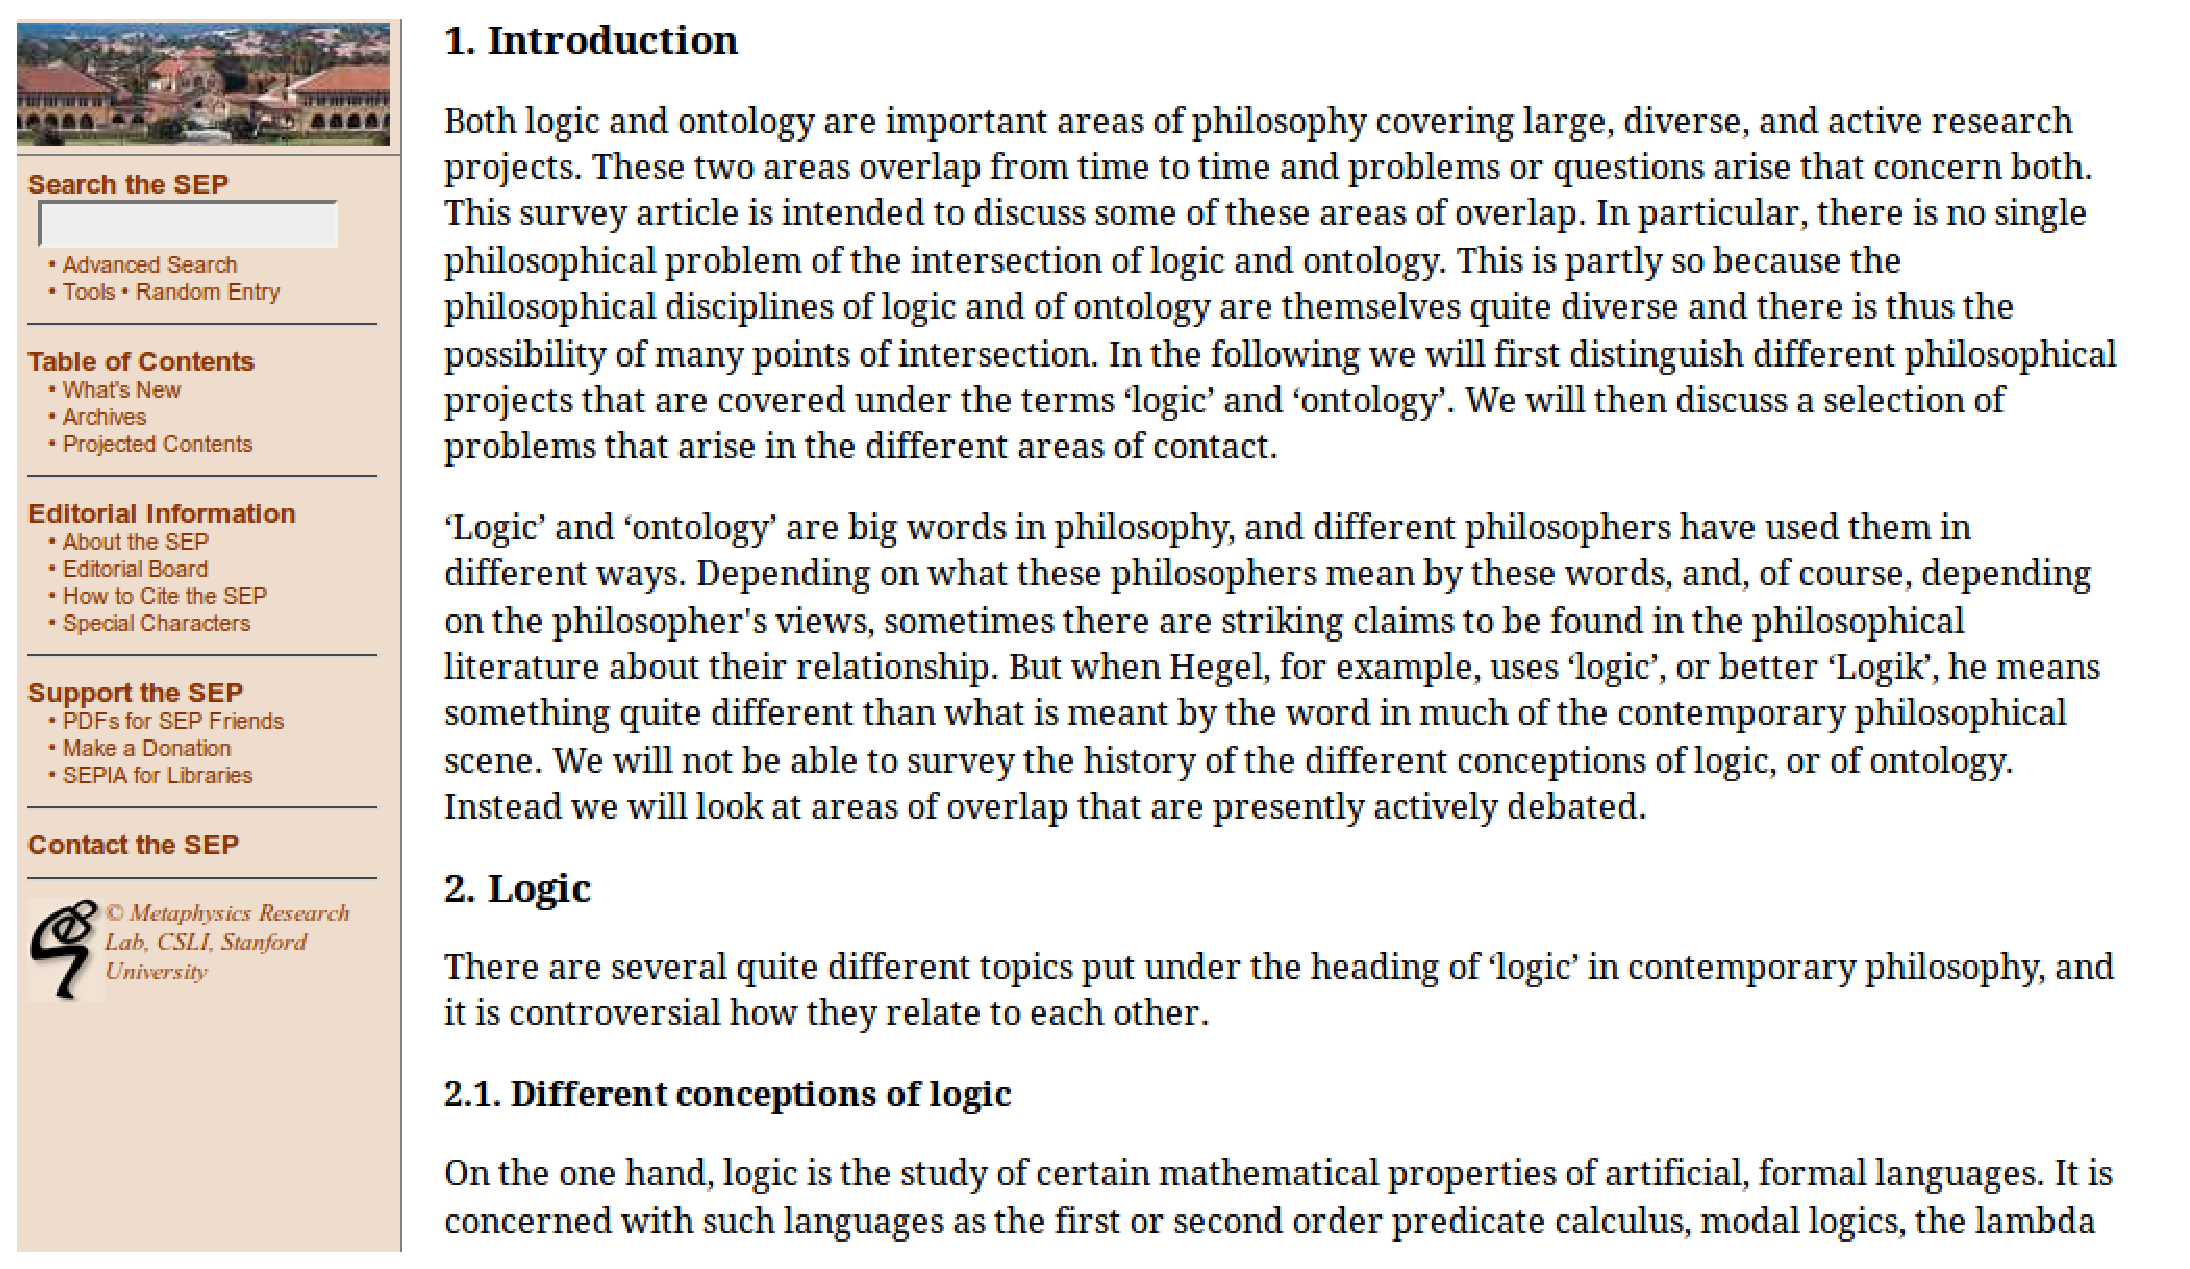
\includegraphics[width=8cm]{graphicswcc/good}
  \end{center}

\end{frame}



\begin{frame}
{Distinguishing the ``good'' from the ``bad'' (I)}  

\begin{itemize}
\item Classification has to be performed automatically
\item ML algorithms usually need manually annotated training data 
\item But: the decision is difficult even for humans and arbitrary to some extent
\end{itemize}
\pause

Experiment: 3 raters, 1000 random documents from German web corpus, using 5-point scale:

 \begin{itemize}
	\item $-2,-1$: document \alert{should not} be in the corpus 
	\item $1, 2$: document \alert{should} be in the corpus 
	\item $0$: undecided\slash document \alert{might or might not} be in the corpus
 \end{itemize}

 \end{frame}

\begin{frame}
{Distinguishing the ``good'' from the ``bad'' (II)}
Results (after training phase of rating of 100 documents together, with several hours of discussion of borderline cases):


  \begin{center}
\scalebox{.8}{
  \begin{tabular}{lrrr}
    \hline
    statistic & early 500 & late 500 & all 1,000 \\
    \hline
    \hline
    raw & 0.566 & 0.300 & \alert<2->{0.433} \\
    $\kappa$ (raw) & $0.397$ & $0.303$ & $0.367$ \\
    $ICC(C,1)$ & $0.756$ & $0.679$ & $\alert<2->{0.725}$ \\
    \hline
    raw ($r\geq0$) & 0.900 & 0.762 & \alert<2->{0.831} \\
    raw ($r\geq1$) & 0.820 & 0.674 & 0.747 \\
    $\kappa$ ($r\geq0$) & $0.673$ & $0.625$ & $\alert<2->{0.660}$ \\
    $\kappa$ ($r\geq1$) & $0.585$ & $0.555$ & $0.598$ \\
    $\kappa$ ($r\geq2$) & $0.546$ & $0.354$ & $0.498$ \\
    \hline
  \end{tabular}
}
  \end{center}

\end{frame}




\begin{frame}{``Good'' vs.\ ``bad'' documents: lists}

   \begin{center}
    \includegraphics[width=8cm]{graphicswcc/rezept}
  \end{center}

\end{frame}



\begin{frame}{``Good'' vs.\ ``bad'' documents: lists (II)}

   \begin{center}
    \includegraphics[width=11cm]{graphicswcc/kunststoff}
  \end{center}

\end{frame}


\begin{frame}{``Good'' vs.\ ``bad'' documents: lists (III)}

   \begin{center}
    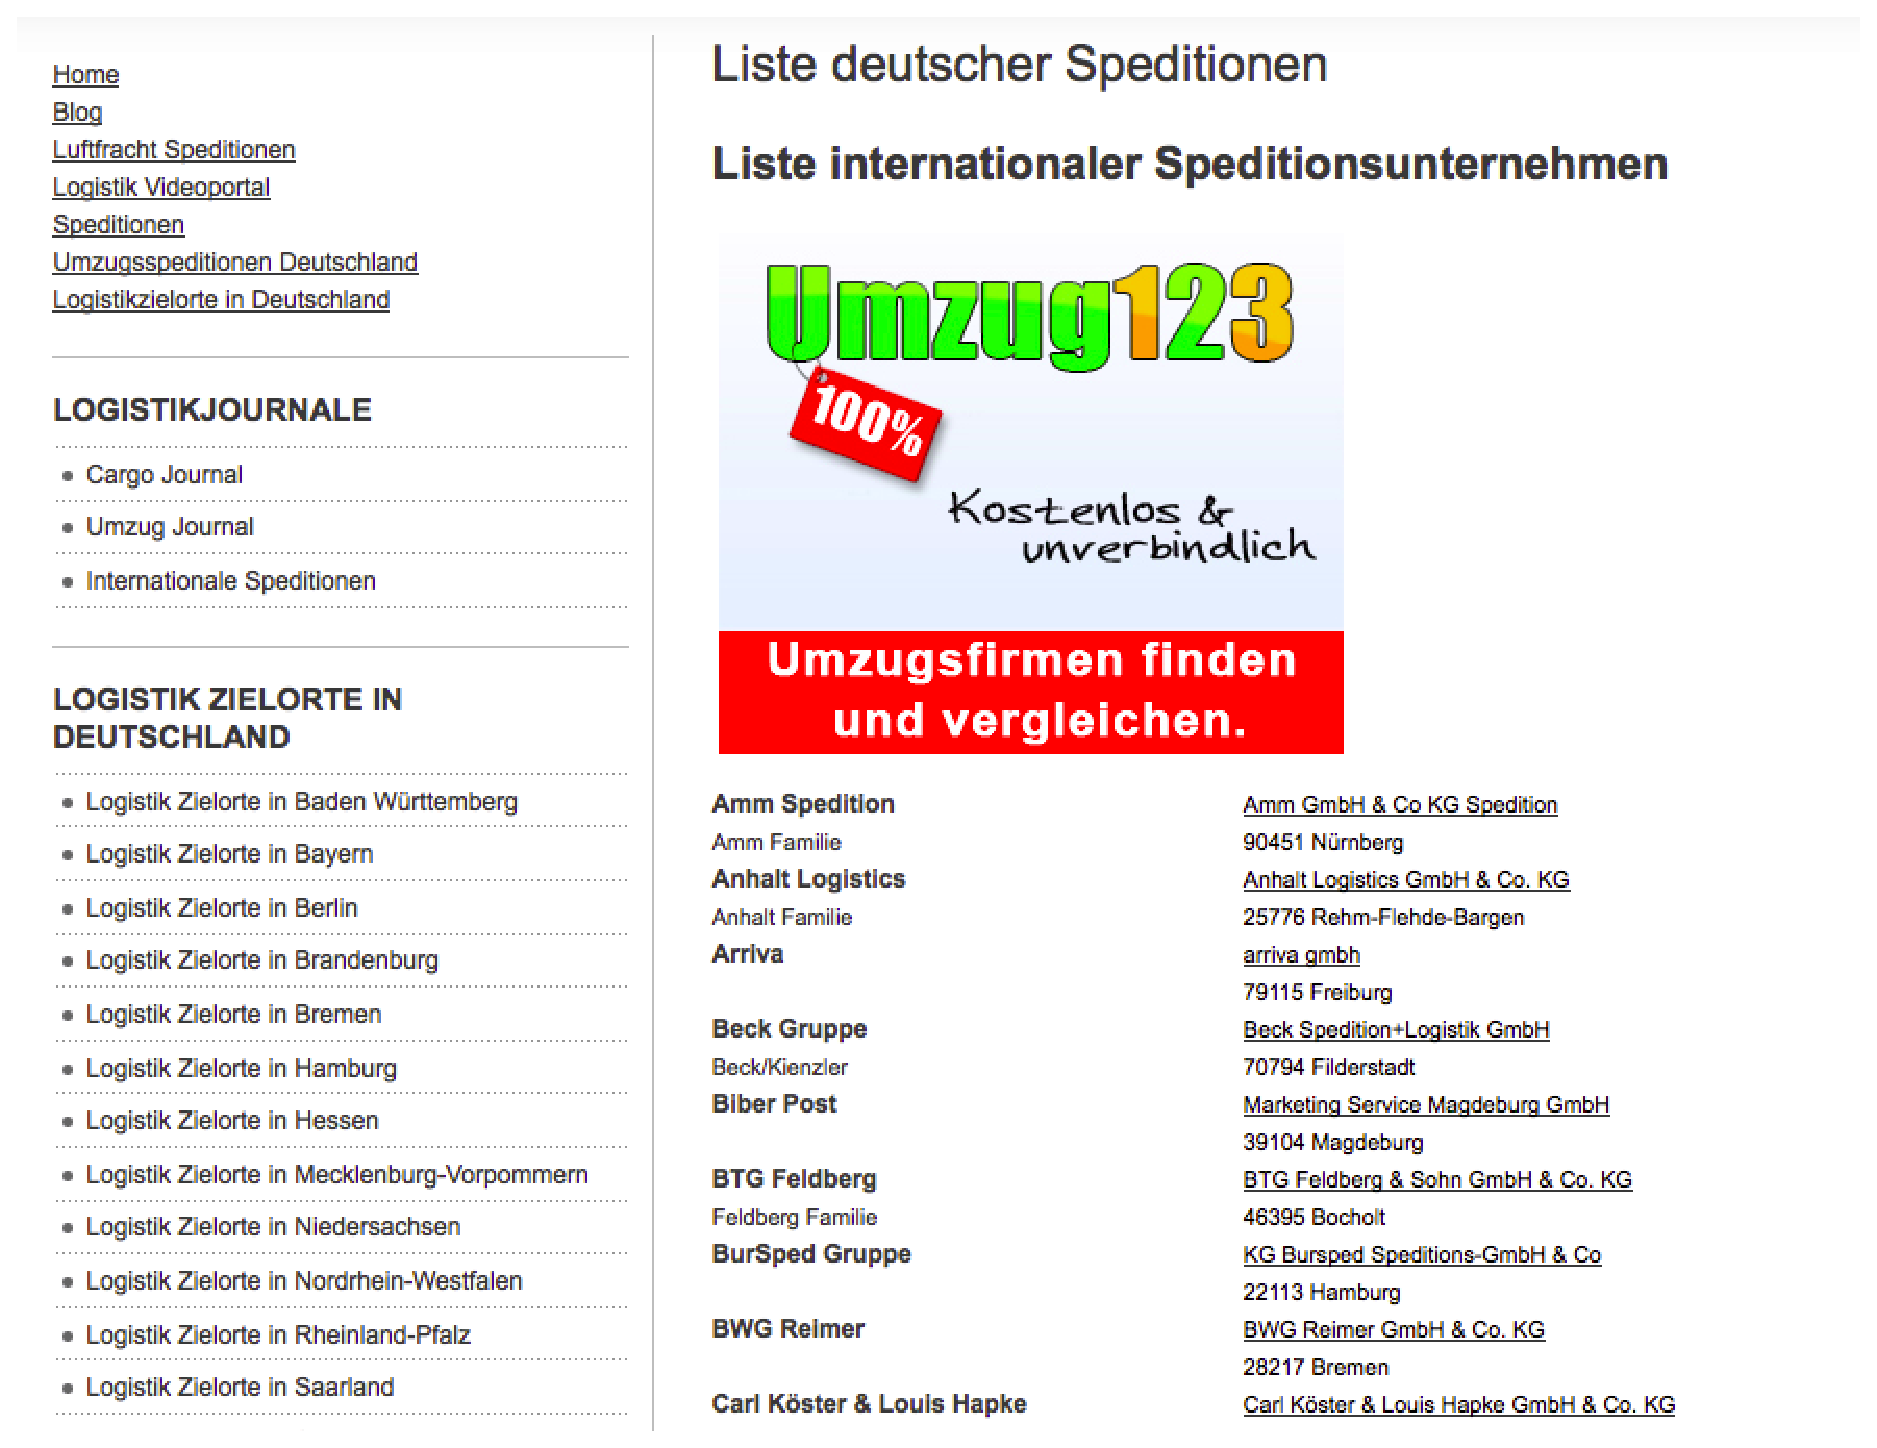
\includegraphics[width=8cm]{graphicswcc/spedition}
  \end{center}

\end{frame}


\begin{frame}
  {Acceptable results?}
  \begin{itemize}
    \item \alert{values below $0.68$ \citep{Krippendorff1980}}
    \item even considering criticism of Krippendorf's magic number\\
      \citep{Carletta1996,BayerlPaul2011}:\\
      \alert{uncomfortably low for ``gold standard''}
    \item more confusion on late data (lower overall quality)
    \item worse: disagreement between corpus designers
    \item acceptance at the threshold $\geq 0$:\\
      A: 78.4\%, R: 73.8\%, S: 84.9\%
  \end{itemize}
\end{frame}

%\subsection{Badness scores}

\begin{frame}
  {General method and idea}
  \begin{itemize}
    \item simple metric with known properties
    \item language-independent, unsupervised\ldots\\
      \alert{does not involve an obviously difficult design decision}
    \item strategy for cleansing: \alert{high recall for everyone},\\
      accept mediocre precision
    \item for retained documents: use as annotation in final corpus,\\
      \alert{allow corpus users to ``set'' precision}
  \end{itemize}
\end{frame}

\begin{frame}
  {Implementation}
  \begin{itemize}
    \item based on ``frequent\slash short word'' method\\
      in language identification \citep{Grefenstette1995}
    \item similar to WaCky \citep{Baroni-ea2009}\\
      but without manually compiled lists of function words
    \item totally unsupervised procedure for crawled data\\
      predominantly in a single language (TLD crawl):
      \begin{itemize}
	\item \alert{training}: get weighted mean and standard deviation\\
	  of relative frequencies of the most frequent words (``profile'')
	\item \alert{production}: calculate for the top $m$ of them\\
	  the ``standardized'' negative deviation for each document\\
	\item clamped and added up: the \alert{Badness score}
      \end{itemize}
  \end{itemize}
\end{frame}


\subsection{Duplication}


\begin{frame}
{Duplicate sentences in a corpus concordance}


Query: \texttt{made a donation}

\vspace{1cm}

   \begin{center}
     \alt<1>{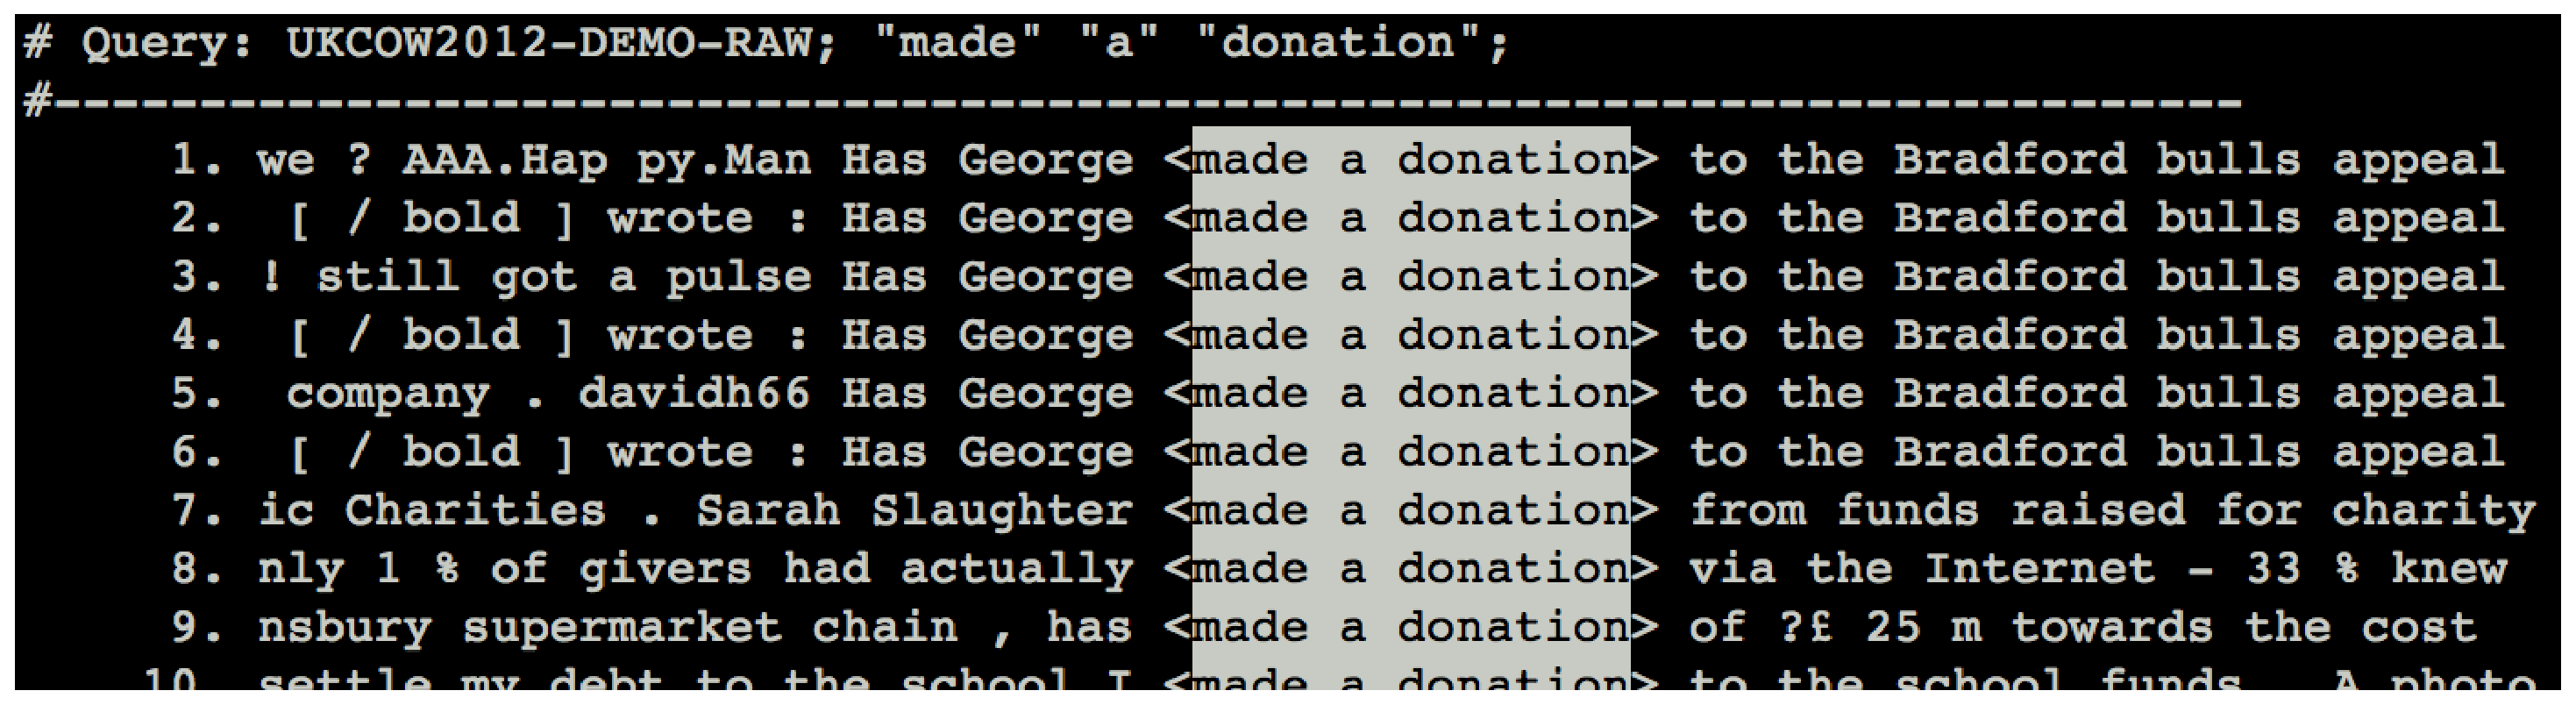
\includegraphics[width=10cm]{graphicswcc/donation}}{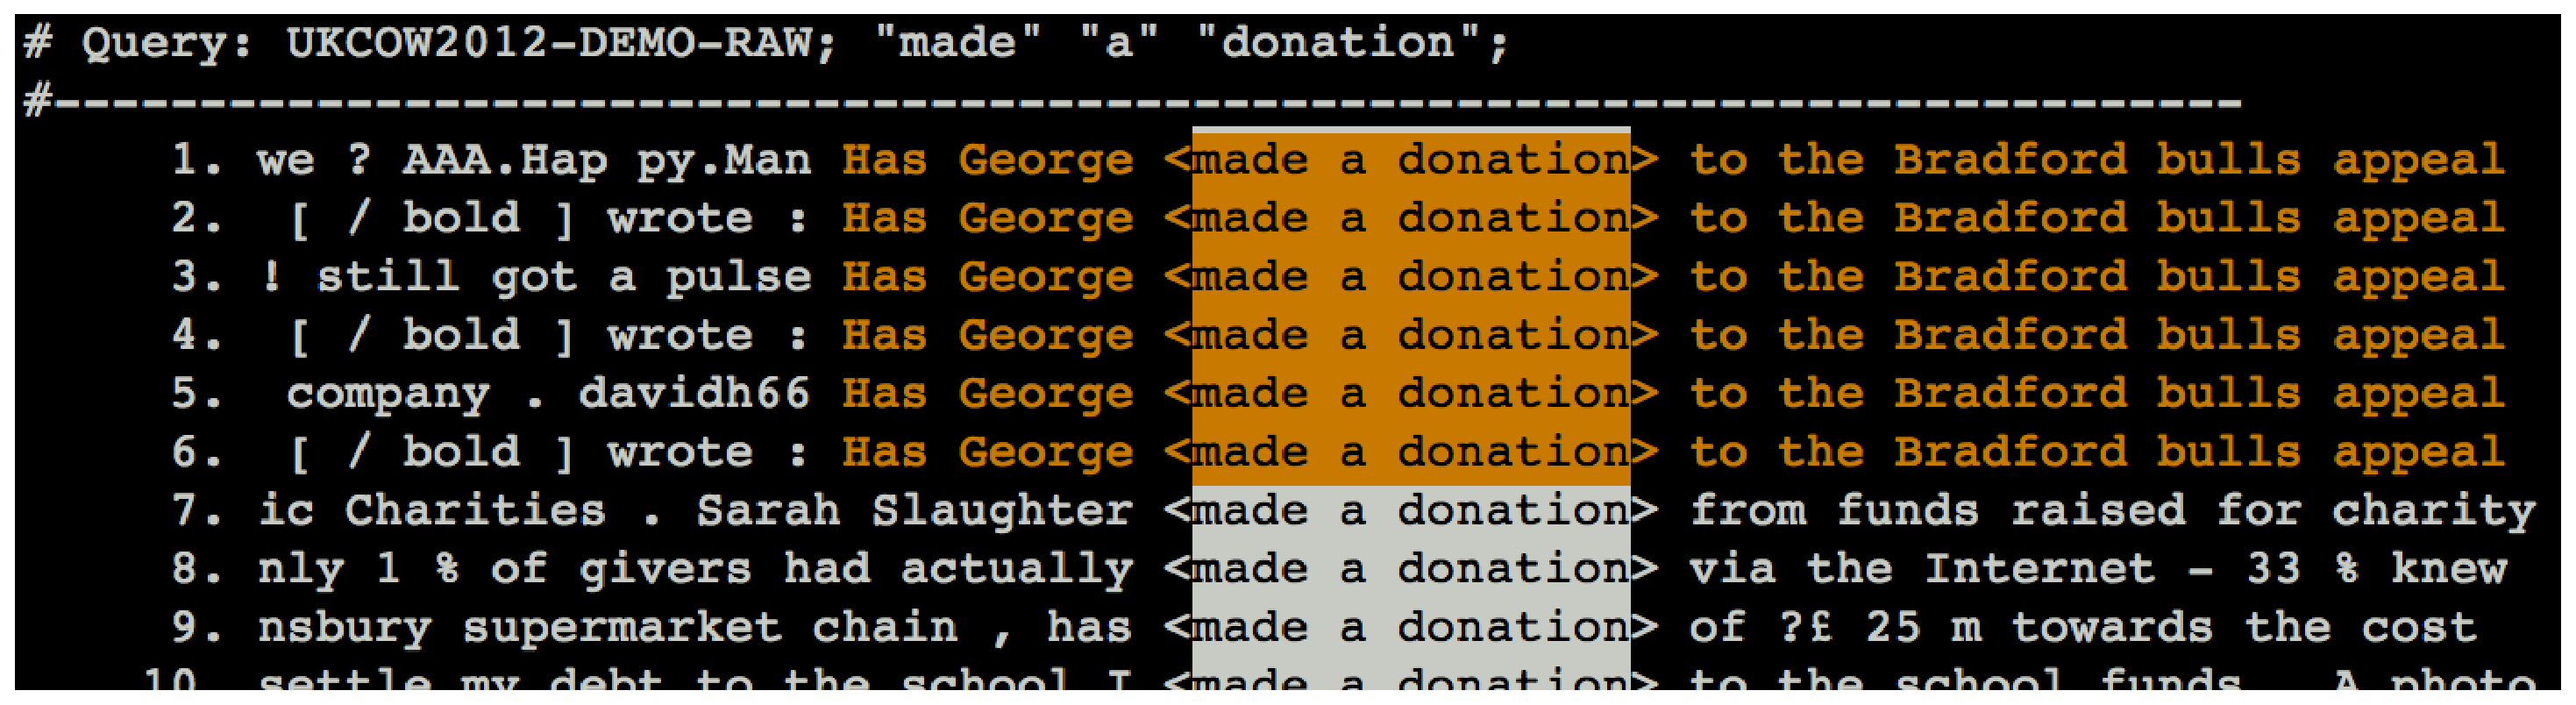
\includegraphics[width=10cm]{graphicswcc/donation2}}\\
   \end{center}  

\pause

\end{frame}



\begin{frame}
   \begin{center}
     
\includegraphics[width=10cm]{graphicswcc/argus2}\\
   \end{center}  
\end{frame}


 \begin{frame}

   \begin{center}
     
\includegraphics[width=8cm]{graphicswcc/george1col2}\\
   \end{center}
\pause
  \begin{center}
     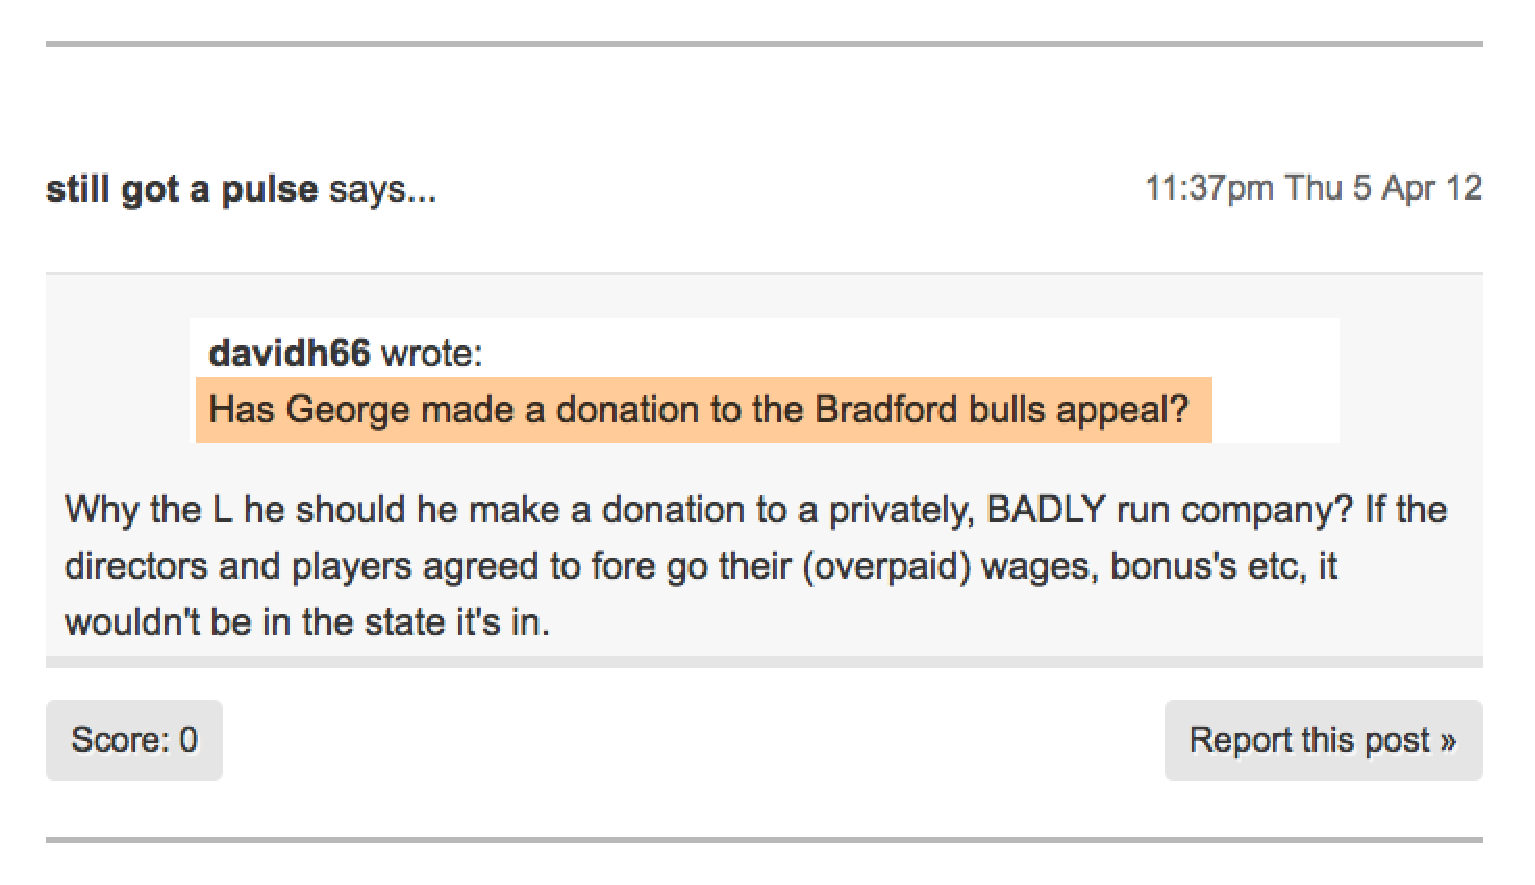
\includegraphics[width=8cm]{graphicswcc/george2col2}\\
   \end{center}

 \end{frame}


 \begin{frame}
   \begin{center}
     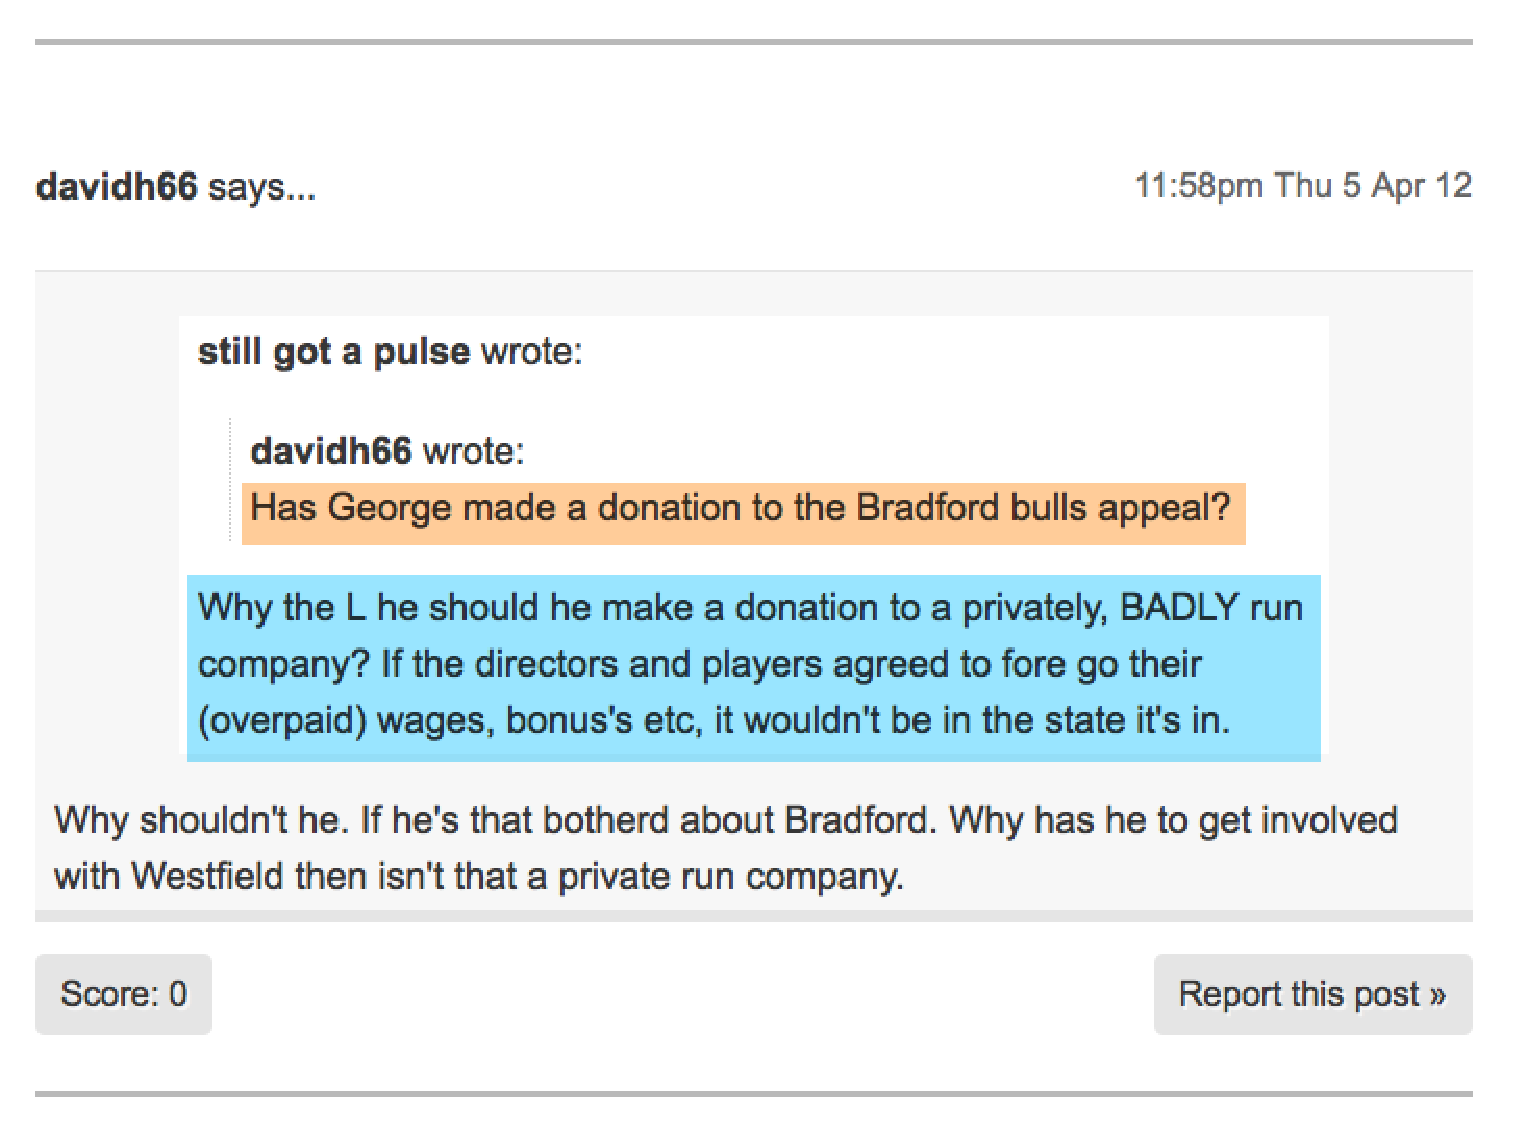
\includegraphics[width=8cm]{graphicswcc/george3col2}\\
   \end{center}
 \end{frame}


 \begin{frame}
   
  \begin{center}
     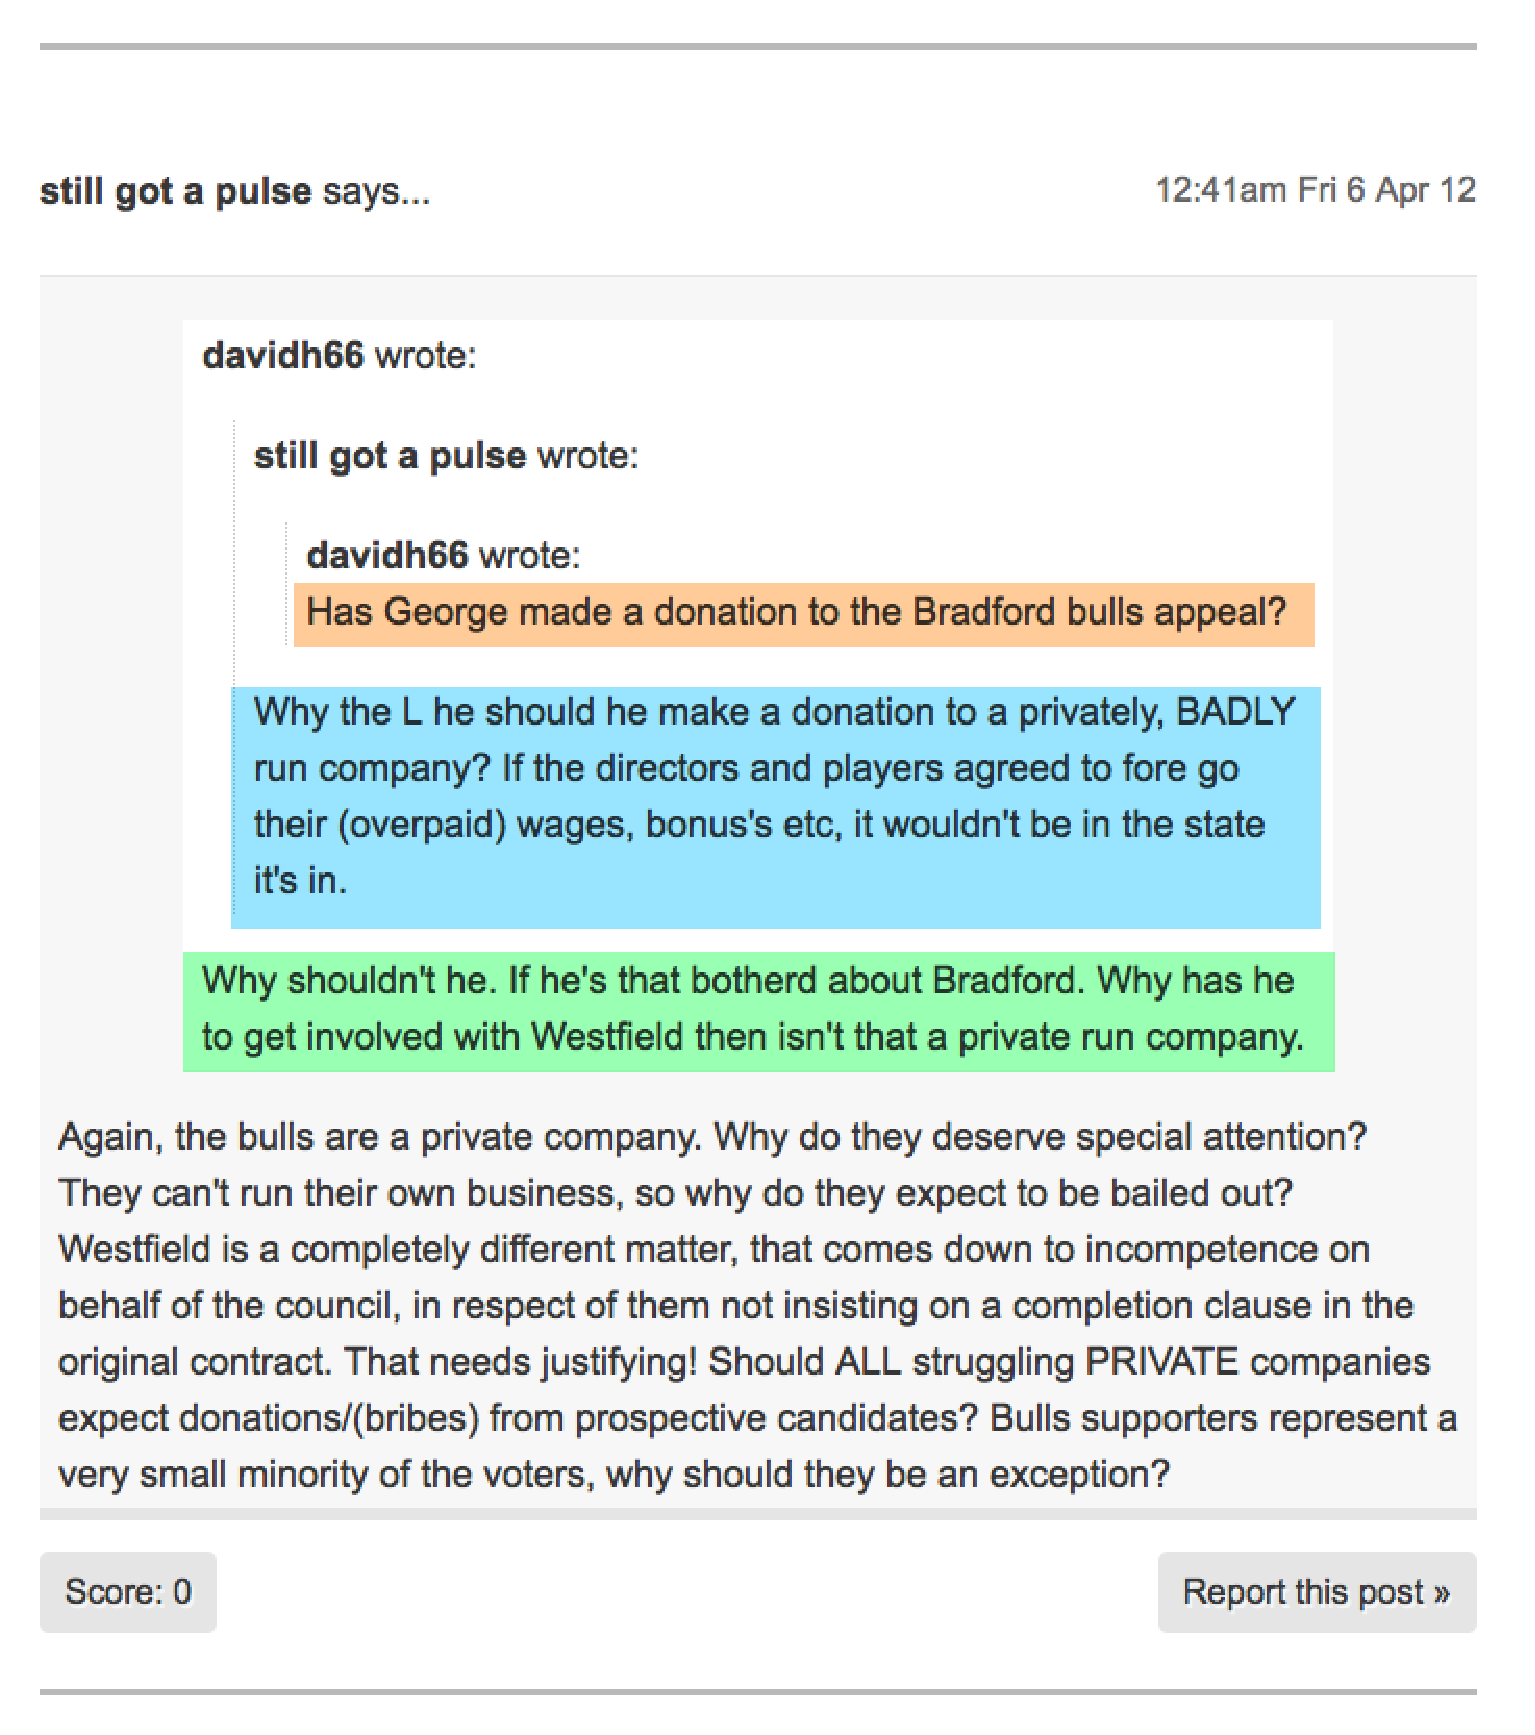
\includegraphics[width=8cm]{graphicswcc/george4col}\\
   \end{center}

 \end{frame}



\begin{frame}
  {Near duplication and inclusion}
  \begin{itemize}
    \item Many web pages are not perfect duplicates of others,\\
      but just \alert{very similar}.
    \item One typical source: slightly edited texts from news agencies\\
      in several newspapers.
    \item Also, some web pages fully contain other web pages (\alert{inclusion}).
    \item Inclusion situation is made worse by typical blog and content management systems.
  \end{itemize}
\end{frame}


% \begin{frame}
%   This is part of a month view of a blog with many postings:
%   \begin{center}
%     \includegraphics[width=8cm]{graphicswcc/lawblog}\\
%     (\url{http://www.lawblog.de/}, 11.10.2011)
%   \end{center}
% \end{frame}

% \begin{frame}
%   But each posting is also available as a single page:
%   \begin{center}
%     \includegraphics[width=8cm]{graphicswcc/lawblog_einzeln}\\
%     {\scriptsize(\url{http://www.lawblog.de/index.php/archives/2011/10/07/erotische-schriften/})}
%   \end{center}
% \end{frame}

%\begin{frame}
%  {Failure of perfect duplicate hashing/fingerprinting}
%  \begin{center}
%    $D_1$ : \alert<3>{Y}esterday\alert<4>{,} I wrote a le\alert<5>{t}ter to my pa\alert<6>{r}ents.\\
%    $D_2$ : \alert<7>{Y}esterday \alert<7>{I} wrote a let\alert<7>{t}er to my par\alert<7>{e}nts.
%  \end{center}
%  \begin{itemize}
%    \item<2> Hashes (\eg, SHA1 -- very, maybe too strong for the given task):
%      \begin{itemize}
%	\item 12d952c23cc3869faead1e1aa6e02b98256e35f8
%	\item 5ad8468fcb45fe07ef420fd87cd360087514d1f1
%      \end{itemize}
%  %  \item <3->Fingerprints using every tenth character:
%  %    \begin{itemize}
%%	\item<3-> $D_1$: \alert<3>{y}\alert<4>{,}\alert<5>{t}\alert<6>{r}
%%	\item<7-> $D_2$: \alert<7>{y}\alert<7>{i}\alert<7>{t}\alert<7>{e}
% %     \end{itemize}
%  \end{itemize}
%\end{frame}
%
%
%%\subsection{Jaccard Coefficients}
%\begin{frame}
%  {Solution -- in principle: Jaccard Coefficients}
%  \begin{itemize}
%    \item One can measure the similarity of two documents as \\
%      \alert{the Jaccard Coefficient of the sets of their n-grams}\\
%      \citep[61,438]{Manning-ea2009}. 
%      \vspace{.2cm}
%    \item Procedure:
%      \begin{itemize}
%	\item Create the documents' word\slash token-n-grams.
%	\item Calculate the \alert{Jaccard Coefficient} of the two sets.
%	\item If it is above a certain threshold, delete the shorter\\
%	  of the two documents.
%      \end{itemize}
%  \end{itemize}
%\end{frame}
%
%\begin{frame}
%  {Example: High similarity with JC over token-bi-grams I}
%  \begin{center}
%    \alert<1>{Yesterday}\alert<1-2>{,} \alert<2-3>{I} \alert<3-4>{wrote} \alert<4-5>{a} \alert<5-6>{letter} \alert<6-7>{to} \alert<7-8>{my} \alert<8-9>{parents}\alert<9>{.}\\
%\vspace{.5cm}
%    $FP(D_1)=$\{\alert<1>{(yesterday;,)}, \alert<2>{(,;i)}, \alert<3>{(i,wrote)}, \alert<4>{(wrote;a)}, \alert<5>{(a;letter)}, \alert<6>{(letter;to)}, \alert<7>{(to;my)}, \alert<8>{(my;parents)}, \alert<9>{(parents;.)}\}\\
%\vspace{.5cm}
%    \onslide<10->{Yesterday I wrote a letter to my parents.\\
%\vspace{.5cm}
%    $FP(D_2)=$\{(yesterday;i), (i,wrote), (wrote;a), (a;letter), (letter;to), (to;my), (my;parents), (parents;.)\}}
%  \end{center}
%\end{frame}
%
%\begin{frame}
%  {Example: High similarity with JC over token-bi-grams II}
%  \begin{center}
%    $FP(D_1)=$\{\alert<2>{(yesterday;,)}, \alert<2>{(,;i)}, \alert<1-2>{(i,wrote)}, \alert<1-2>{(wrote;a)}, \alert<1-2>{(a;letter)}, \alert<1-2>{(letter;to)}, \alert<1-2>{(to;my)}, \alert<1-2>{(my;parents)}, \alert<1-2>{(parents;.)}\}\\
%\vspace{.5cm}
%$FP(D_2)=$\{\alert<2>{(yesterday;i)}, \alert<1-2>{(i,wrote)}, \alert<1-2>{(wrote;a)}, \alert<1-2>{(a;letter)}, \alert<1-2>{(letter;to)}, \alert<1-2>{(to;my)}, \alert<1-2>{(my;parents)}, \alert<1-2>{(parents;.)}\}\\
%\vspace{1cm}
%$J(D_1,D_2)=\frac{|D_1\cap D_2|}{|D_1\cup D_2|}=\frac{7}{10}=0.7$
%%$J(D_1,D_2)=\frac{\alert<1>{|D_1\cap D_2|}}{\alert<2>{|D_1\cup D_2|}}=\frac{\alert<1>{7}}{\alert<2>{10}}=0.7$
%  \end{center}
%\end{frame}
%
%\begin{frame}
%  {Example: Low similarity with JC over token-bi-grams}
%  \begin{center}
%    $FP(D_2)=$\{\alert{(yesterday;i)}, (i,wrote), (wrote;a), (a;letter), (letter;to), \alert{(to;my)}, (my;parents), (parents;.)\}\\
%\vspace{0.5cm}
%$D_3=$Yesterday I read a book to my niece.\\
%\vspace{0.5cm}
%$FP(D_3)=$\{\alert{(yesterday;i)}, (i,read), (read;a), (a;book), (book;to), \alert{(to;my)}, (my;niece), (niece;.)\}\\
%\vspace{1cm}
%$J(D_2,D_3)=\frac{|D_2\cap D_3|}{|D_2\cup D_3|}=\frac{2}{14}=0.14$
%  \end{center}
%\end{frame}
%
%\begin{frame}
%  {Can it be done?}
%   \begin{itemize}
%     \item 10,000,000 documents\\[1ex]
%     \item $\approx \frac{10,000,000^2}{2} = 5 \times 10^{13}$ comparisons\\[1ex]
%     \item at $1\mu s$ per comparison: $\approx$ 579 days
%     \item \graw{But $1\mu s$ is faster than available processors can do it.}
%   \end{itemize}
%
%\pause
%
%Solution:  
%
%
%\begin{itemize}
%\item Do not \textbf{calculate} JC for each pair of documents.
%\item Instead, \textbf{estimate} the JC \citep{Broder-ea1997}.
%\item Technique is known as \textit{w-Shingling}.
%\end{itemize}
%
%\end{frame}
%
%
%



 \begin{frame}
{Near-duplicate detection with \texttt{w-shingling}}

\texttt{w-shingling} does not tell us which amount of duplication\\
is acceptable in a corpus.

\begin{itemize}
 \item<1-> Setting a particular JC as a threshold for keeping/discarding\\
   a document is ultimately an arbitrary choice
    \begin{itemize}
    \item Design decision by corpus builders. 
    \end{itemize}
\item<2-> Web corpora will probably always contain a certain amount\\
  of duplication
    \begin{itemize}
    \item many other corpora do, too
    \end{itemize}

\item<3-> Strategies to cope with duplication:
   \begin{itemize}
   \item If compatible with research question:\\
     work with sentence-wise uniq'ed corpora.
   \item Or work with unique (not too short) concordance lines.
   \end{itemize}


\end{itemize}
 
 \end{frame}


\subsection{Linguistic post-processing}


\begin{frame}
  {Noise in web corpora: sources}

  \begin{enumerate}
 \item <1-> properties of web-documents, e.\,g.
    \begin{itemize}
    \item quasi-spontaneous writing situations with (often)\\
      casual language, typos, non-standard spellings,\\
      improper use of whitespace and punctuation
    \item text contributed by non-native speakers 
    \item a large lexicon with many out-of-vocabulary items
   \end{itemize}
  \item<2-> the structure of the WWW and its technologies, e.\,g.
    \begin{itemize}
    \item duplicated text, boilerplate
    \end{itemize}
  \item<2-> shortcomings in post-processing, e.\,g.
    \begin{itemize}
    \item HTML/code-stripping, tokenization 
    \end{itemize}
  \end{enumerate}
\end{frame}



% \begin{frame}{Example: spelling variants}
  
% \begin{figure}[h]
%   \centering
%   \scalebox{.7}{
%     \begin{tabular}{lc@{\hspaceThis{XXXXXXXXXXX}}lrr}
%       Correct form (frequency)& & Misspelled form & N & edit distance \\
%       \hline
%       &&\node{a}{\alert{u}bernimmt} & 81 & 1 \\
%       &&\node{b}{überni\alert{n}mmt}& 6 & 1\\
%       &&\node{c}{übernimm\alert{n}t}& 1 & 1\\
%       &&\node{d}{überni\alert{e}mt} & 6 & 1\\
%       &&\node{e}{\alert{ö}bernimmt} & 6 & 1\\
%       &&\node{f}{übernim\alert{n}mt}& 5 & 1\\
%       &&\node{h}{übernimm\alert{e}t}& 11 & 1\\
%       \node{x}{übernimmt (297440)}&&\node{i}{überni\alert{eh}mt} & 2 & 2\\
%       &&\node{j}{überni\alert{e}mt} & 6 & 1\\
%       &&\node{k}{überni\alert{h}mt} & 17 & 1\\
%       &&\node{l}{überni\alert{iiiiiiimmmmm}mmt} & 1 & 12\\
%       &&\node{m}{überni\alert{o}mmt}& 4 & 1\\
%       &&\node{n}{übernim\alert{rn}t}& 4 & 2\\
%       &&\node{p}{überni\alert{u}mmt}& 2 & 1\\
%       &&\node{q}{überni\alert{nn}t} & 2 & 2\\
%       &&\node{r}{übernimm\alert{t}t}& 2 & 1\\
%       &&\node{o}{\ldots}
%     \end{tabular}
% %    \anodeconnect[r]{x}[l]{a}
% %    \anodeconnect[r]{x}[l]{b}
% %    \anodeconnect[r]{x}[l]{c}
% %    \anodeconnect[r]{x}[l]{d}
% %    \anodeconnect[r]{x}[l]{e}
% %    \anodeconnect[r]{x}[l]{f}
% %    \anodeconnect[r]{x}[l]{h}
% %    \anodeconnect[r]{x}[l]{i}
% %    \anodeconnect[r]{x}[l]{j}
% %    \anodeconnect[r]{x}[l]{k}
% %    \anodeconnect[r]{x}[l]{l}
% %    \anodeconnect[r]{x}[l]{m}
% %    \anodeconnect[r]{x}[l]{n}
% %    \anodeconnect[r]{x}[l]{p}
% %    \anodeconnect[r]{x}[l]{q}
% %    \anodeconnect[r]{x}[l]{r}
% %    \anodeconnect[r]{x}[l]{o}
%   }



% \end{figure}

% \end{frame}


\begin{frame}{Example: text produced by non-native speakers}
\begin{center}
     \includegraphics[width=11cm]{graphicswcc/walkman}\\
   \end{center}
\end{frame}



\begin{frame}
{Noise in linguistic post-processing}

Most available natural language processing tools expect standard written language as input.

\begin{itemize}
\item Many tokenizers expect proper use of whitespace,\\
  casing and punctuation.
\item Part-of-speech taggers expect properly tokenized text as input.
\item POS-taggers usually perform worse on unknown items\\
     (tokenization errors, misspellings, out-of-vocabulary items).
\item Proper tokenization and POS tagging is normally the basis\\
  for higher-level linguistic annotation\\
  (parsing, sense disambiguation etc.).
\end{itemize}
\end{frame}



\begin{frame}
{Should noise be ``normalized away''?}

What exactly is ``noise'' in the first place?

\begin{itemize}
\item No general definition of ``noise'' that suits all purposes
\item What counts as noise in one task may be valuable data\\
  in another task
\end{itemize}
\end{frame}


\begin{frame}
{Can noise be ``normalized away''?}


In large web corpora, noise would have to be eliminated automatically, without human interaction.\\[1ex]

\begin{itemize}
\item viable in some cases:
  \begin{itemize}
  \item e.\,g.\ correcting run-together words\\
   \texttt{a \alert{lot.I} don't think} $\rightarrow$\  \texttt{a lot. I don't think} 
  \end{itemize}
\vspace{1cm}
\pause
\item but not an easy task in other cases:
  \begin{itemize}
  \item e.\,g.\ spelling correction\\
   \texttt{I didn't spend much time with \alert{Bibble}.} $\rightarrow$ \textit{Bubble}?
  \end{itemize}
\end{itemize}
\end{frame}



%\begin{frame}
%  {Non-destructive normalization}
%Our approach: do as much as possible non-destructively\\
%(i.\,e.\, do not alter the original data).
%\begin{itemize}
%\item Normalization-as-annotation
%\item But there are limits to this approach imposed\\
%  by the indexing/query architecture.
%\end{itemize}
%\end{frame}
%
%
%\begin{frame}{Non-destructive orthographic normalization}
%
%\setlength{\columnsep}{1cm}
%\begin{multicols}{2}
%  \scalebox{.8}{
%   \ttfamily
%    \begin{tabular}{llll}
%      & \textbf{Word} & \textbf{POS} & \textbf{Lemma} \\
%      \cline{2-4}
%      & The     & DT    & the   \\
%      & FA      & NP    & FA    \\
%      & does    & VBZ   & do    \\
%      & \alert{abosolutley}&\alert{JJ}&\alert{$<$unknown$>$}\\
%      & nothing & NN    & nothing       \\
%      & to      & TO    & to    \\
%      & help    & VB    & help  \\
%      & Clubs   & NNS   & club  \\
%    \end{tabular}
%  }
%
%\columnbreak
%\onslide<2->{
% \scalebox{.8}{
%    \ttfamily
%    \begin{tabular}{llll}
%      & \textbf{Word} & \textbf{POS} & \textbf{Lemma} \\
%      \cline{2-4}
%      & The     & DT    & the   \\
%      & FA      & NP    & FA    \\
%      & does    & VBZ   & do    \\[0.8ex]
%      \multicolumn{4}{l}{$<$norm from="{}abosolutley"$>$} \\[0.8ex]
%      & \alert{absolutely} &\alert{ADV}&\alert{absolutely} \\[0.8ex]
%      \multicolumn{4}{l}{$<$/norm$>$} \\[0.8ex]
%      & nothing & NN    & nothing       \\
%      & to      & TO    & to    \\
%      & help    & VB    & help  \\
%      & Clubs   & NNS   & club  \\
%    \end{tabular}
%  }
%}
%\end{multicols}
%
%%\vspace{.2cm}
%
%\begin{multicols}{2}
%{\footnotesize
%Original text: spelling error, POS-tagging error, no lemma
%
%\columnbreak
%\onslide<2->{
%Normalized text: standard spelling, correct POS and lemma, original spelling preserved as meta data
%}
%}
%\end{multicols}
%
%\end{frame}


\begin{frame}
  {Quality of linguistic annotation in web corpora}

Automatic annotation may be concern, e.\,g.\

\begin{itemize}
\item Do not take type counts in web corpora at face value.
  \begin{itemize}
  \item There are many \textit{hapax legomena} due to tokenization issues.
  \end{itemize}
\item POS tagging of web corpora does not quite reach\\
  accuracy levels in the upper 90\%
  \begin{itemize}
  \item but many POS taggers do not reach such accuracy levels\\
    on traditional, out-of-domain texts either
  \end{itemize}
\end{itemize}

\pause

But:

\begin{itemize}
\item Depending on the specific research question,\\
  some or all of these problems by irrelevant.
\item Anyway, in many scenarios, there is no alternative\\
  to working with web corpora.
\item \alert{And do not expect the situation to be perfect with other corpora!}
\end{itemize}

\end{frame}





\section{COW14, COW16, and COCO15}

\subsection{Current focus at COW's}

\begin{frame}
	{Technology COW14\slash COW16}

	\begin{itemize}
	  \item texrex-behindthecow: advanced web page cleaner
	  \item various normalization tools (own development)
	  \item sentence-wise language filtering with LangID.py + heuristics
	  \item annotation with TreeTagger, SMOR, FreeLing, Marmot, MaltParser, Stanford NER, Berkeley Parser\\
	    (topological model by Cheung \& Penn (2009) etc.

	  \vspace{0.5cm}
	   
	  \item Parallel computing makes the impossible possible:\\
		for example, parsing DECOW16 takes 2 days on
		FU Berlin HPC instead of 450 days on a single machine.
	\end{itemize}
\end{frame}

\begin{frame}
	{Details on the methodology}
	\centering
	
\includegraphics[height=0.7\textheight]{graphics/wcc}
\end{frame}

\begin{frame}
  {COW14\slash COW16 facts}
  \begin{center}
    \begin{tabular}[h]{lrrr}
      \hline
            & G tokens & M sentences & M documents \\
      \hline
      \hline
      DE & 20.5 & 807 & 17.1 \\
      EN & 16.8 & 608 & 9.2 \\
      ES & 7.3 & &      5.0 \\
      NL & 6.8 & 312 &  5.0 \\
      FR & 9.0 & 329 &  6.9 \\
      SV & 8.6 & 406 &  6.4 \\
      \hline
    \end{tabular}
  \end{center}
\end{frame}



\subsection{COW quality control}

\begin{frame}
  {DECOW and ENCOW 14\slash 16: Example of improvements to annotation quality}
  \begin{itemize}
    \item 3,866 manual additions to TreeTagger lexicon (DE)
    \item two-pass tagging with lemmatization of unknown items by SMOR (DE)
    \item Dependency parses from IMS Stuttgart (by FU Berlin for EN)

	\vspace{0.5cm}

    \item Named entities (DE, EN)

    \begin{itemize}
		\item NER quality for DE evaluated by Lea Helmers (HU Berlin)
		\item quality depended highly on register
		\item standard written: $prec=0.76$ $rec=0.56$
		\item spontaneous written: $prec=0.53$ $rec=0.32$
      \end{itemize}
  \end{itemize}
\end{frame}



\begin{frame}
  {DECOW14A: TreeTagger and Mate-Morphology}
  Post-hoc evaluation of 10.000 tokens (from sentences):\\
  TreeTagger was excellent, Mate morphology horrible, replaced by Marmot
  \vspace{0.5cm}
  \begin{center}
    \scalebox{0.8}{
      \begin{tabular}[h]{lrrrrrrrr}
	\hline
	   & POS & Case & Num & Gend & Comp & Per & Tense & Mod \\
	\hline
	\hline
	correct $\approx$ & 0.97 & 0.83 & 0.9 & 0.79 & 0.9 & 0.9 & 0.87 & 0.83 \\
	\hline
      \end{tabular}
    }
  \end{center}
 
\end{frame}


%\begin{frame}
%	{Evaluation nach Leipziger Art: Satzlängen}
%	\centering
%	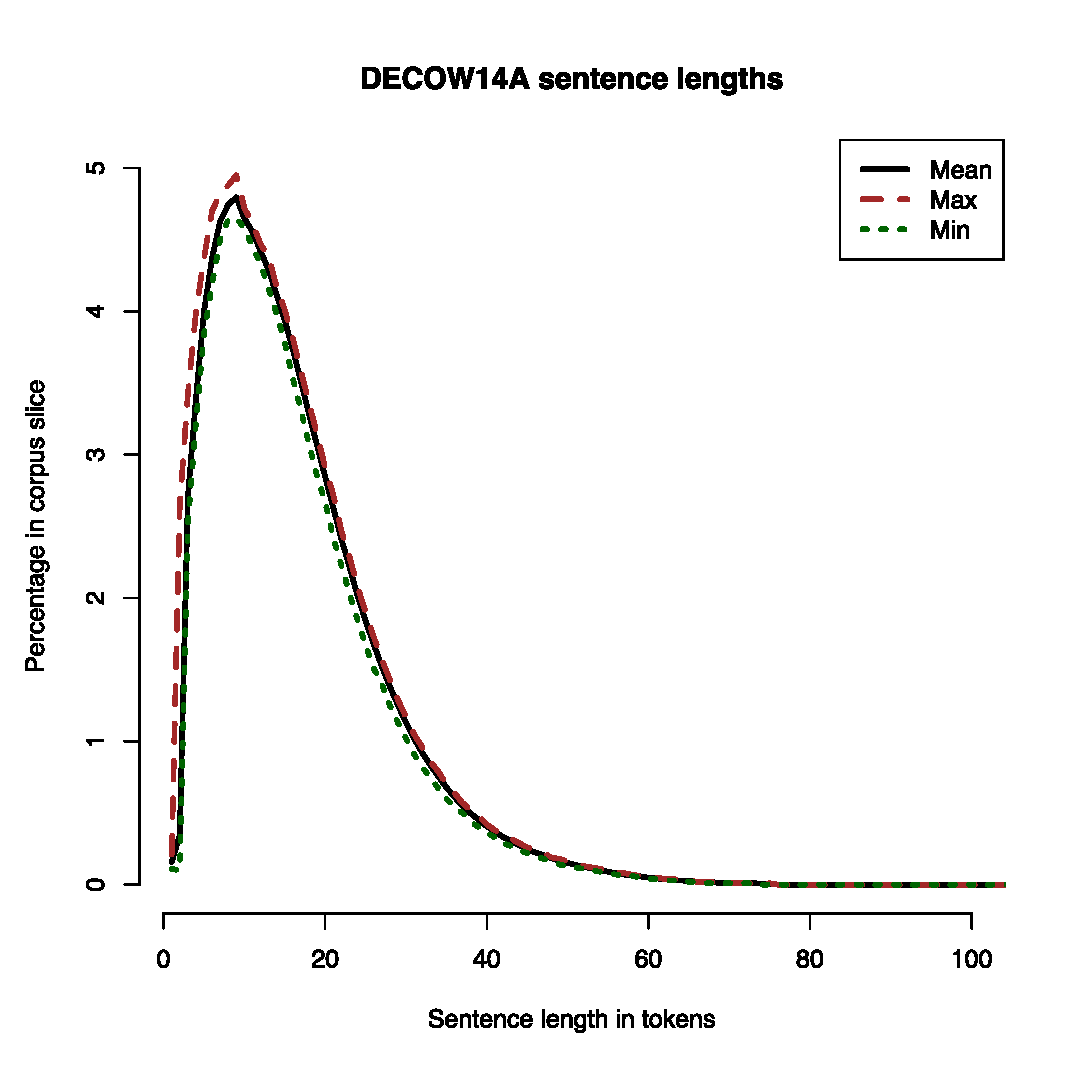
\includegraphics[height=0.8\textheight]{graphics/s_de}
%\end{frame}
%
%\begin{frame}
%	{Evaluation nach Leipziger Art: Satzlängen}
%	\centering
%	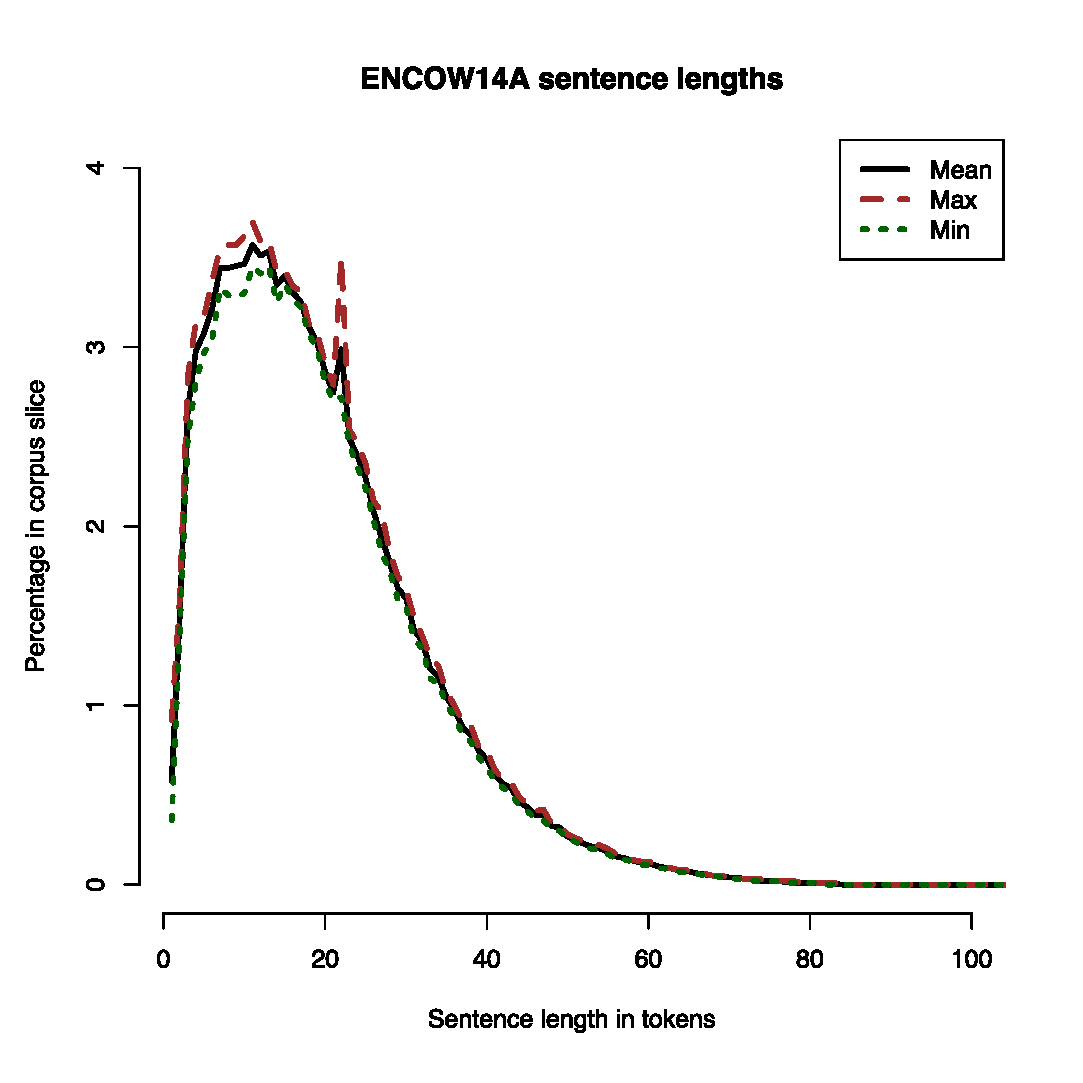
\includegraphics[height=0.8\textheight]{graphics/s_en}
%\end{frame}
%
%\begin{frame}
%	{Evaluation nach Leipziger Art: Satzlängen}
%	\centering
%	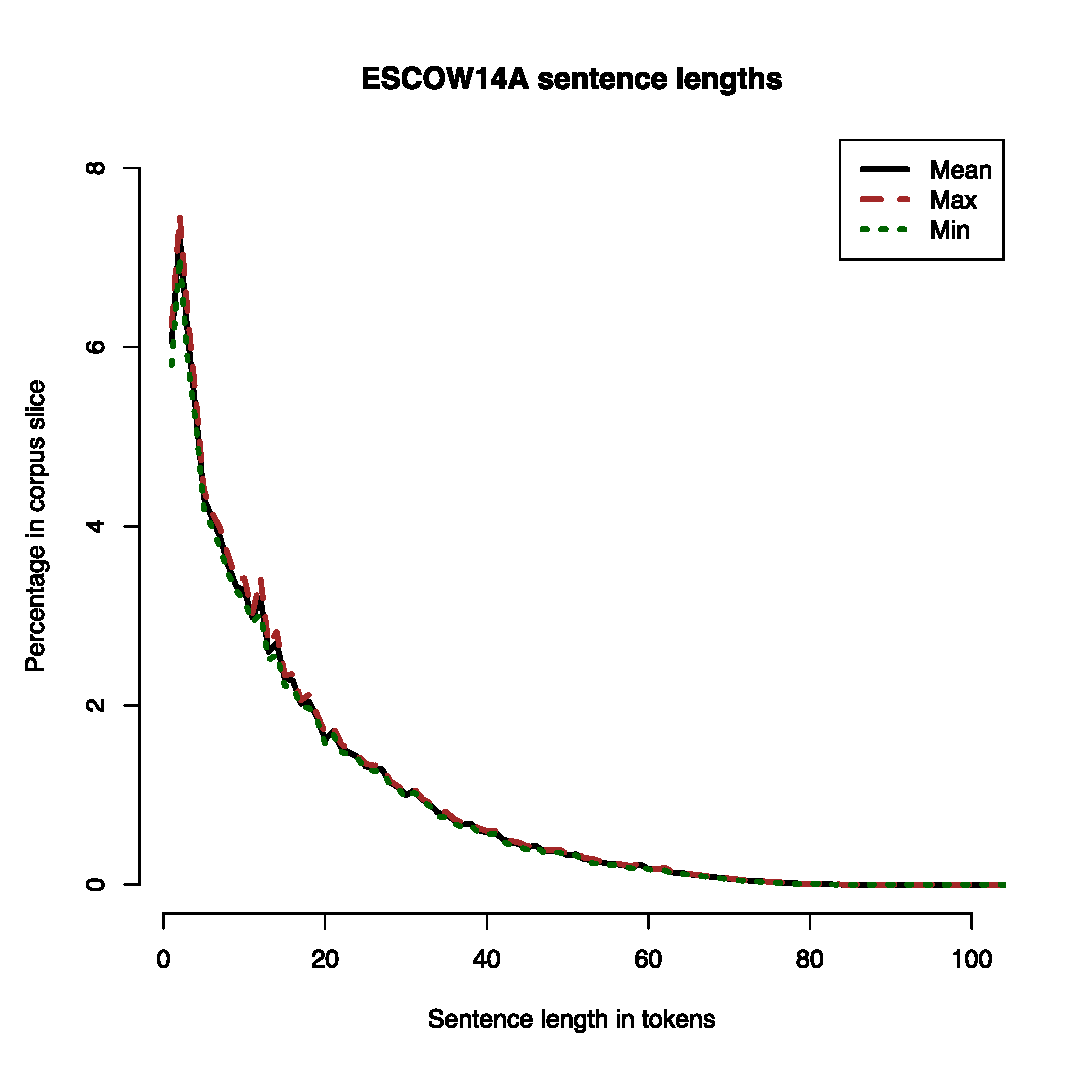
\includegraphics[height=0.8\textheight]{graphics/s_es}
%\end{frame}
%
%\begin{frame}
%	{Evaluation nach Leipziger Art: Satzlängen}
%	\centering
%	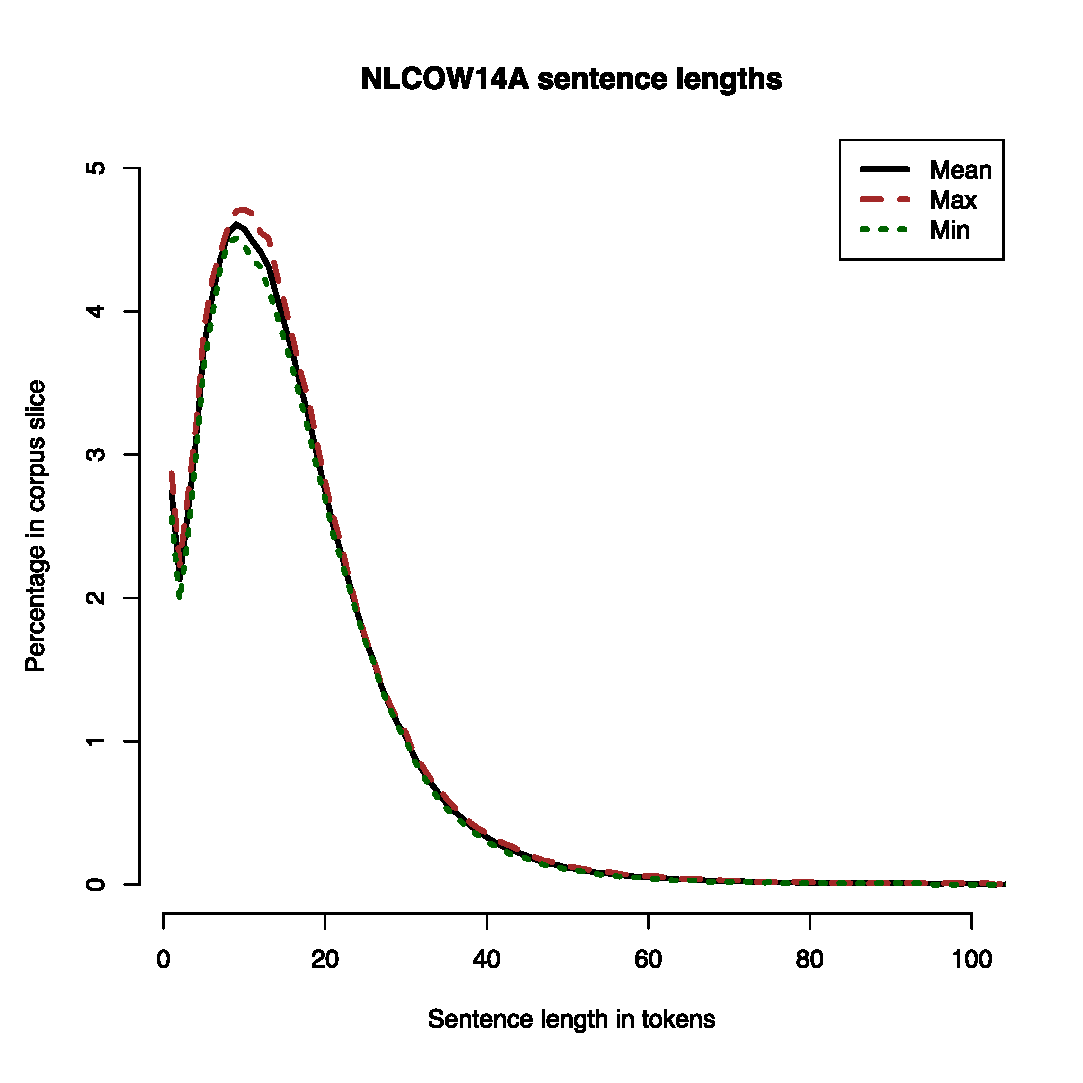
\includegraphics[height=0.8\textheight]{graphics/s_nl}
%\end{frame}
%
%\begin{frame}
%	{Evaluation nach Leipziger Art: Satzlängen}
%	\centering
%	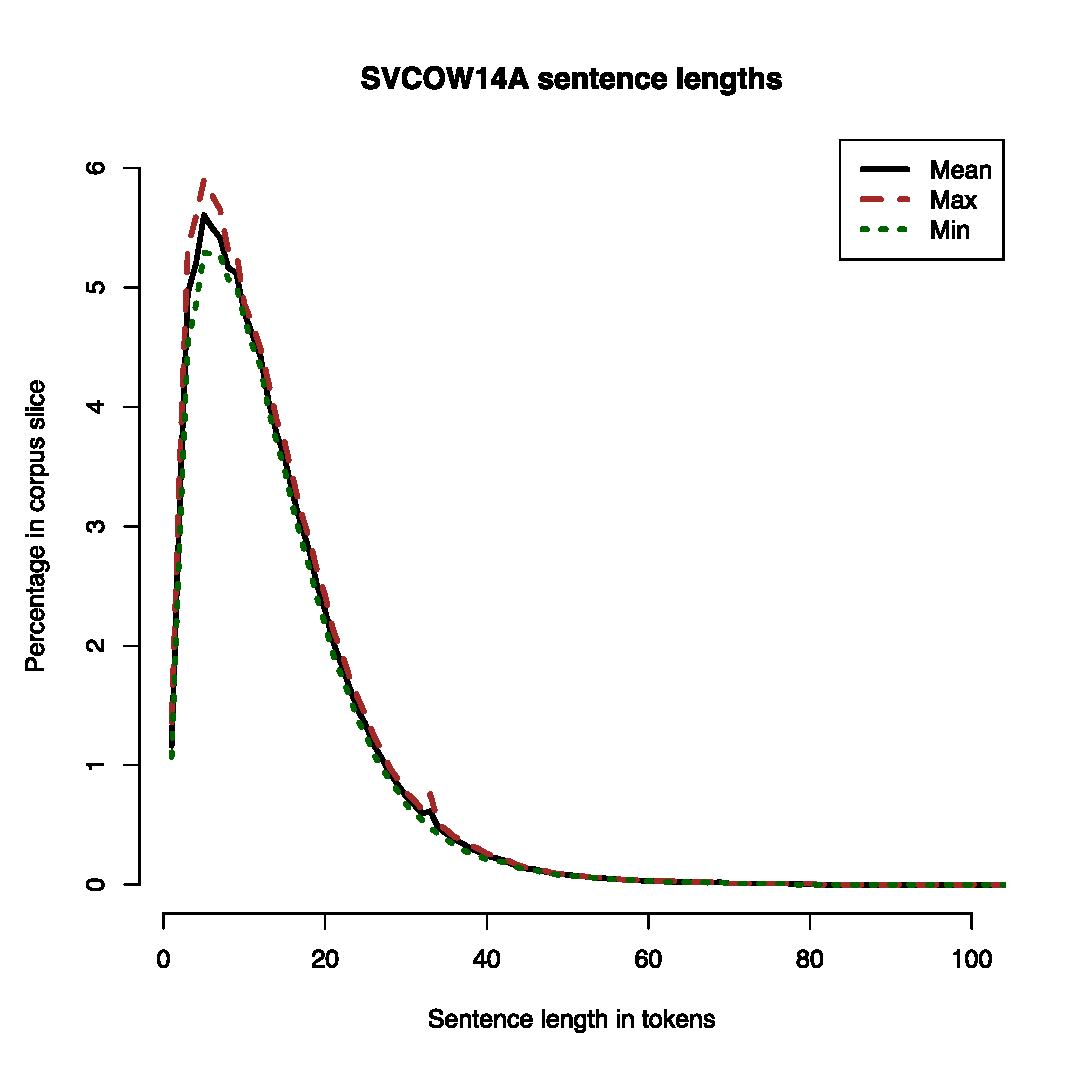
\includegraphics[height=0.8\textheight]{graphics/s_sv}
%\end{frame}


\subsection{COW14\slash 16 corpus composition}

\begin{frame}
  {Number of different web hosts in corpus}
  \begin{center}
    \scalebox{0.9}{
      \begin{tabular}[h]{lrrr}
	\hline
	corpus & hosts & M documents & docs\slash host\\
	\hline\hline
	    DE& 676,424 &  17.1         &  25\\
	    EN& 336,408 &  9.2          &  27\\
	    ES& 158,325 &  5.0          &  32\\
	    FR& 242,801 &  5.0          &  21\\
	    NL& 427,157 &  6.9          &  16\\
	    SV& 255,772 &  6.4          &  25\\
	\hline
      \end{tabular}
    }
  \end{center}
\end{frame}

\begin{frame}
  {Top-level domains}
  \begin{center}
    \scalebox{0.8}{
      \begin{tabular}[h]{cr||cr||cr}
	\multicolumn{2}{c||}{DE} &  \multicolumn{2}{c||}{EN} & \multicolumn{2}{c}{ES} \\
	.de & 16,318,117 & .uk  & 5,409,255 & .es & 3,850,185 \\
	.ch &    511,314 & .com & 2,115,574 & .cl & 303,013  \\
	.at &    29,8091 & .org & 729,899   & .ar & 267,775  \\
	    &            & .edu & 397,317   & .mx & 233,058  \\
	    &            & .net & 203,191   & .cu & 62,725   \\
	    &            & .gov & 139,323   & .co & 54,947   \\
	    &            & .ca  & 81,629    & .pe & 49,390   \\
	    &            & .au  & 45,005    & .ve & 35,552   \\
	    &            & .us  & 40,803    & .uy & 26,779   \\
	    &            & .nz  & 9,207     & .cr & 26,611   \\
	    &            & .ie  & 8,974     & .ec & 19,972   \\
	    &            & .in  & 8,061     & .com& 16,168   \\
      \end{tabular}
    }
  \end{center}
\end{frame}

\begin{frame}
  {Text quality by TLD}
  Distribution of text quality classes in DE14\slash 16\\
  \begin{center}
    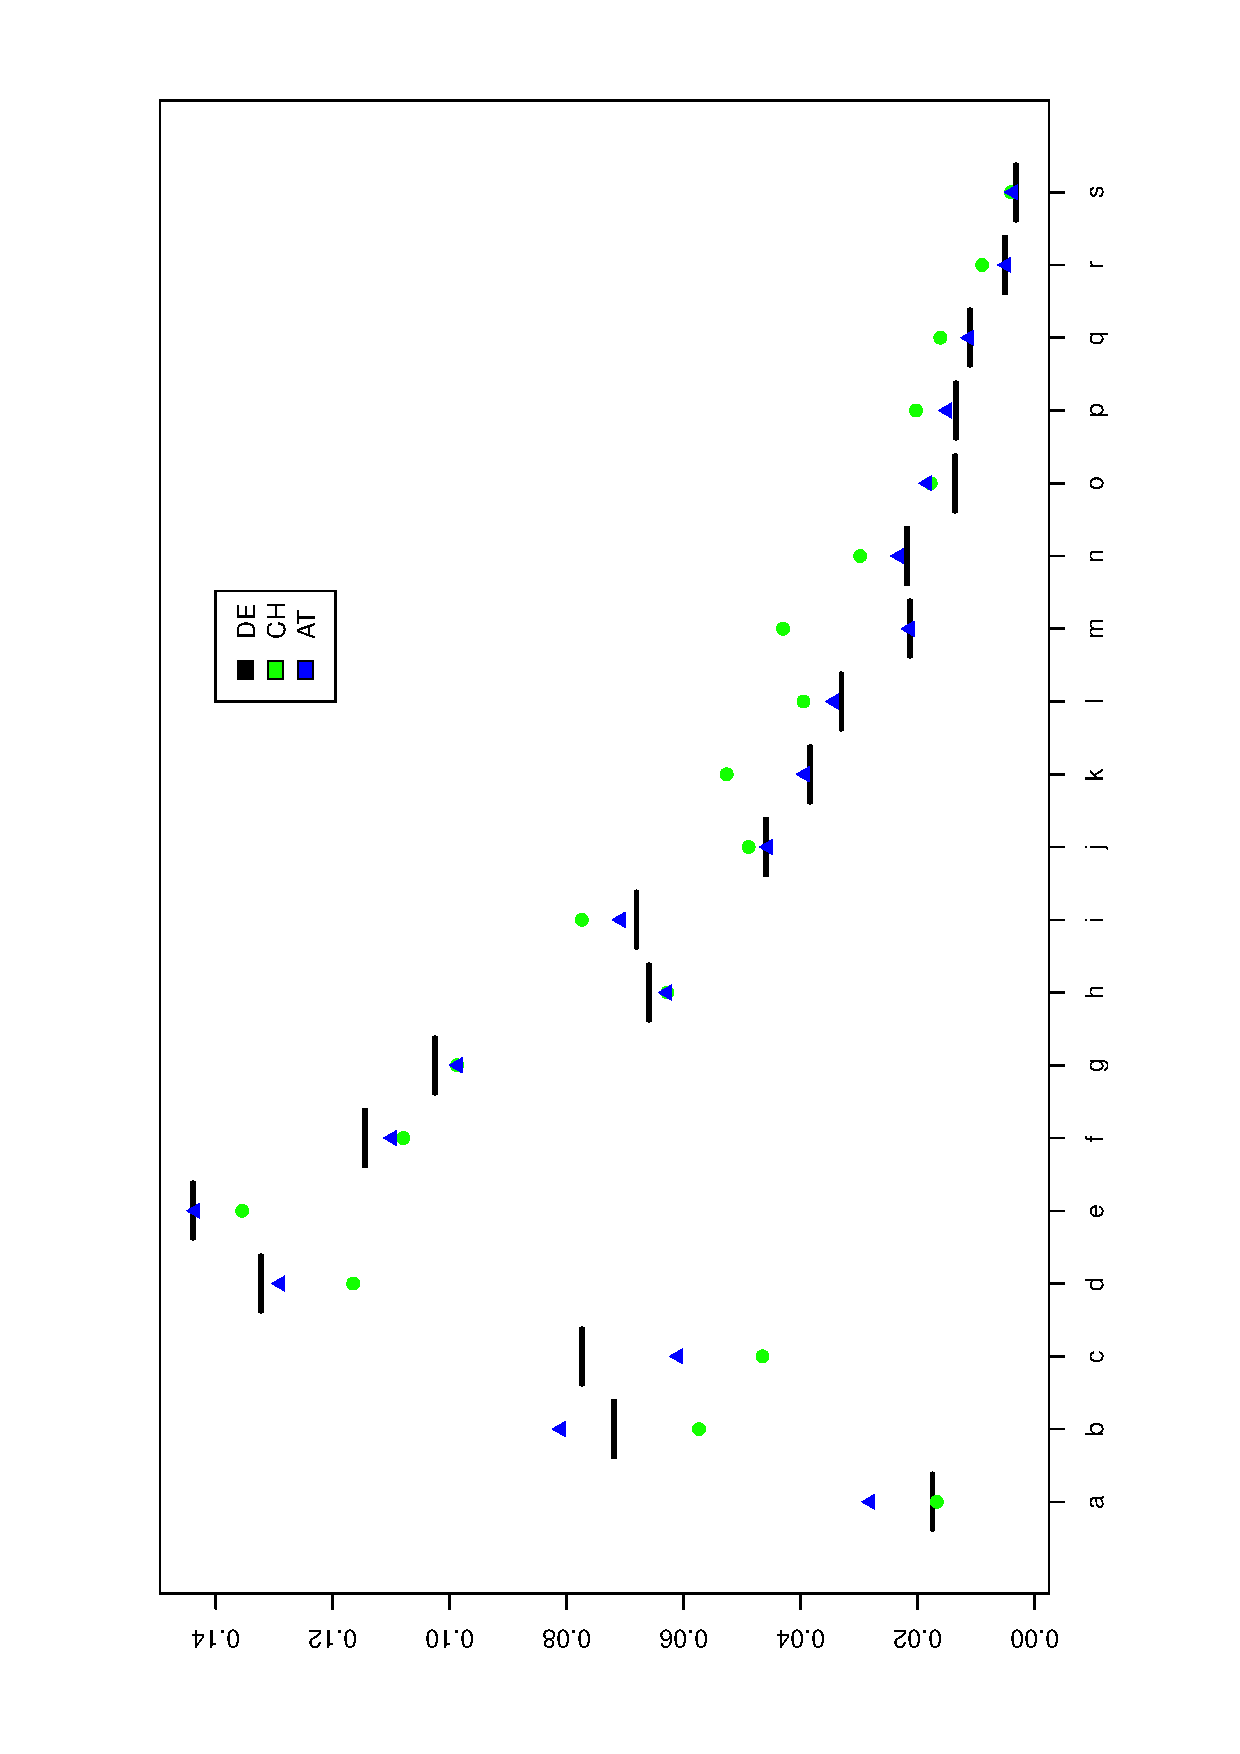
\includegraphics[width=0.5\textwidth,angle=270]{graphics/bdh}
  \end{center}
\end{frame}

\begin{frame}
  {Last-Modified header}
  Distribution of last-modified years\\
  \begin{center}
    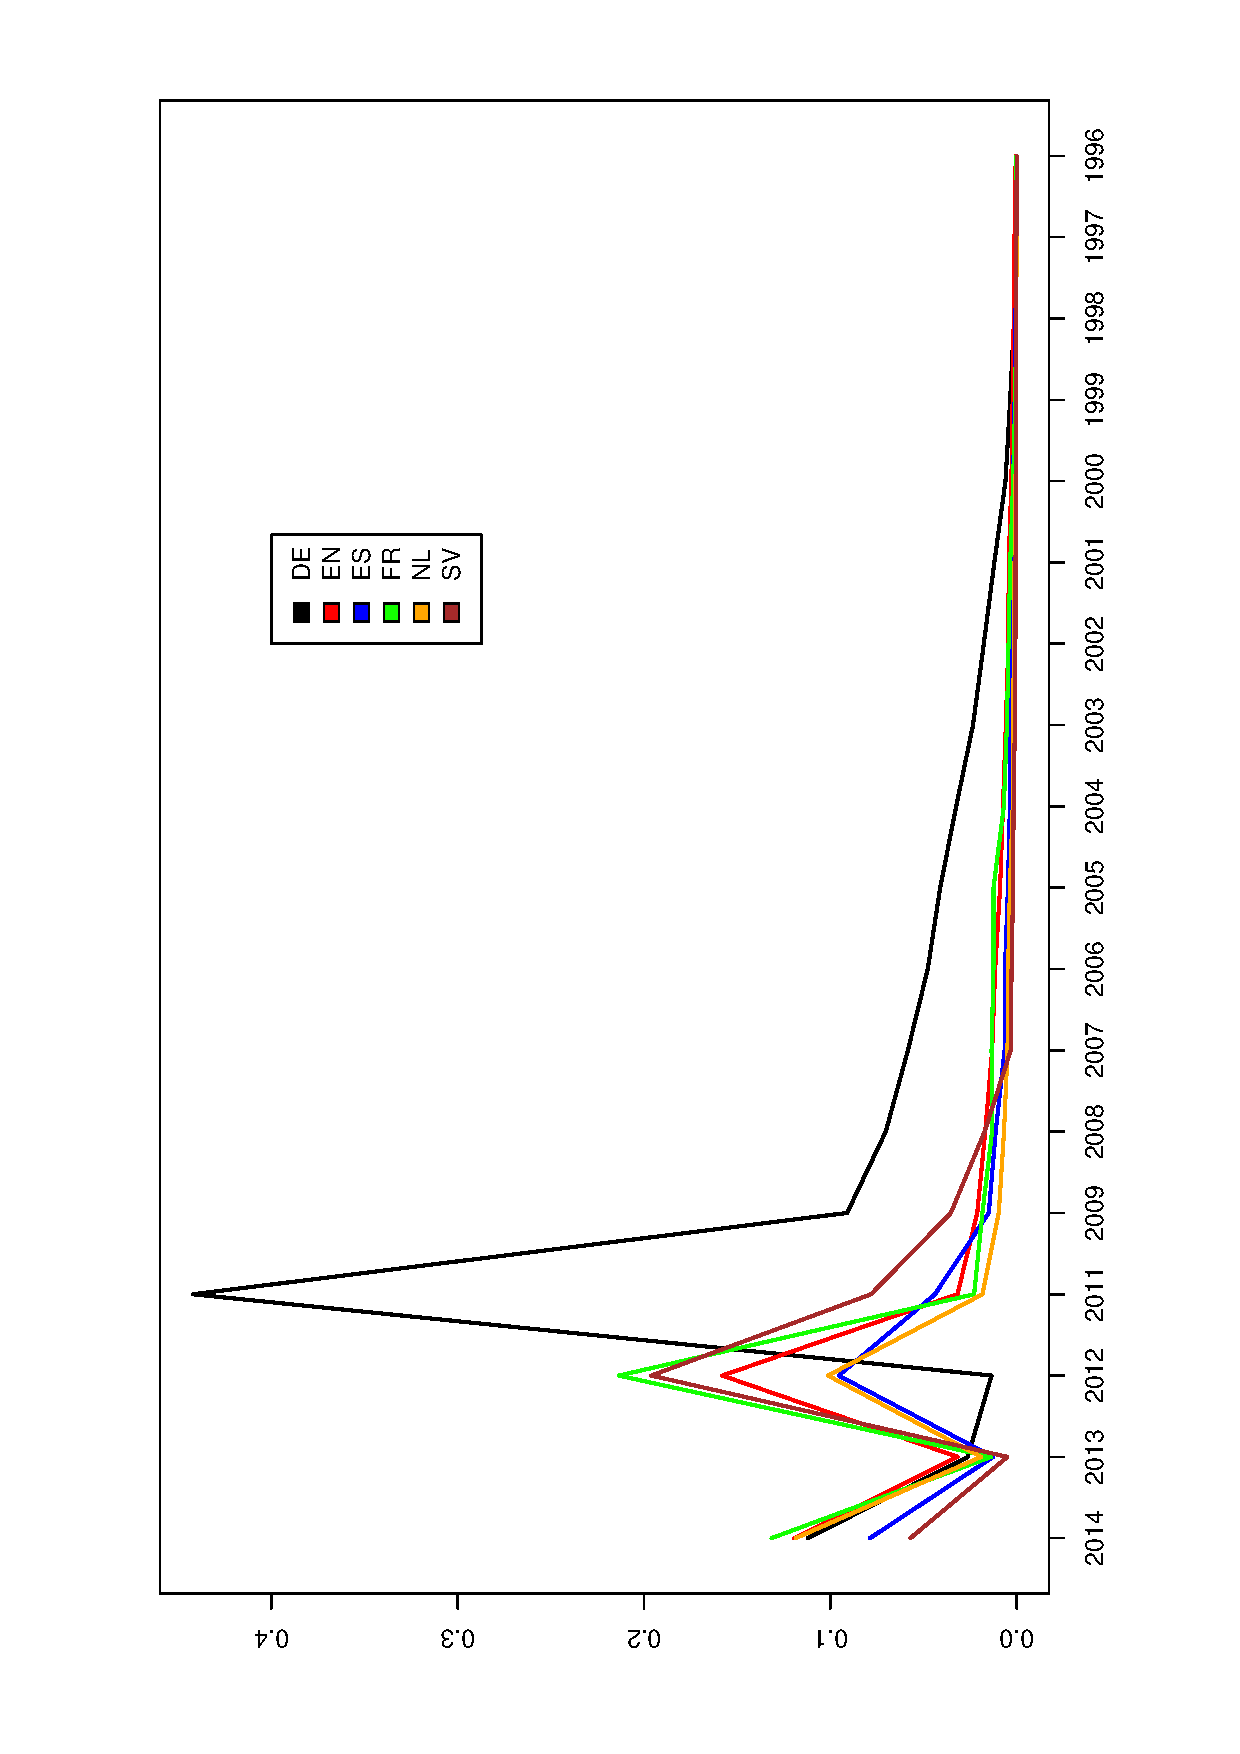
\includegraphics[width=0.5\textwidth,angle=270]{graphics/lastmod}
  \end{center}
\end{frame}


\subsection{COWCat}

\begin{frame}
  {Taxonomy of web document text types}
  \begin{itemize}
    \item based on EAGLES/Sharoff
    \item multiple dimensions, no \textit{genres}
    \item only categories with a potential influence\\on grammatical features
    \item Aim, Audience, Authorship, Domain, Mode
  \end{itemize}
\end{frame}

\begin{frame}
  {Experiment for German}
  \begin{itemize}
    \item 4 raters
    \item 800 documents
    \item training phase: 100 documents, 2 meetings
  \end{itemize}
\end{frame}

\begin{frame}
  {Results}
  Agree and $\kappa$ (Cohen) for two raters with highest agreement
  \vspace{0.5cm}
  \begin{center}
    \begin{tabular}[h]{lrrrr}
      \hline
      & Aim (5) & Aud (3) & Auth (5) & Mode (4) \\
      \hline
      \hline
      Agree & 0.82 & 0.77 & 0.78 & 0.92 \\
      $\kappa$ & 0.58 & 0.53 & 0.71 & 0.82 \\
      \hline
    \end{tabular}
  \end{center}
\end{frame}

\begin{frame}
  {Confusion: Aim (Spanish)}
  \vspace{0.5cm}
  \begin{center}
    \scalebox{0.8}{
      \begin{tabular}[h]{r|rrrrr}
	&  Di & Fi&  If & Is & Re\\
	\hline
      Di& 253 &  0&  20 &  4 &  2\\ 
      Fi&   0 &  2&   0 &  0 &  0\\ 
      If&  78 &  0&  92 &  6 &  2\\ 
      Is&  10 &  0&   2 &  8 &  0\\ 
      Re&   7 &  0&   1 &  2 & 10\\ 
      \end{tabular}
    }
  \end{center}
\end{frame}

\begin{frame}
  {Confusion: Audience (Spanish)}
  \vspace{0.5cm}
  \begin{center}
    \scalebox{0.8}{
      \begin{tabular}[h]{r|rrr}
        &  Ge & In & Pr \\ 
	\hline
      Ge& 426 & 32 &  9 \\ 
      In&  15 &  5 &  4 \\ 
      Pr&   4 &  1 &  4 \\ 
      \end{tabular}
    }
  \end{center}
\end{frame}

\begin{frame}
  {Confusion: Authorship (Spanish)}
  \vspace{0.5cm}
  \begin{center}
    \scalebox{0.8}{
      \begin{tabular}[h]{r|rrrrr}
        &  Co & Mu & Sf & Sm&  Un \\ 
	\hline
      Co&  40 &  0 &  1 &  5&  18 \\ 
      Mu&   0 & 37 &  0 &  4&  12 \\ 
      Sf&   0 &  0 & 19 &  1&   4 \\ 
      Sm&   0 &  2 &  1 & 42&  11 \\ 
      Su&   0 &  1 &  3 &  6&  18 \\ 
      Un&  12 & 14 &  9 & 24& 216 \\ 
      \end{tabular}
    }
  \end{center}
\end{frame}

\begin{frame}
  {Confusion: Mode (Spanish)}
  \vspace{0.5cm}
  \begin{center}
    \scalebox{0.8}{
      \begin{tabular}[h]{r|rrrr}
         & Bm & Qs & Sp &  Wr \\
	 \hline
      Bm & 11 &  4 &  0 &   8 \\ 
      Qs &  3 &  6 &  1 &   4 \\ 
      Sp &  0 &  0 &  8 &   3 \\ 
      Wr &  2 &  3 &  2 & 445 \\ 
      \end{tabular}
    }
  \end{center}
\end{frame}

\begin{frame}
  {TLD-Vergleich}
  \centering
  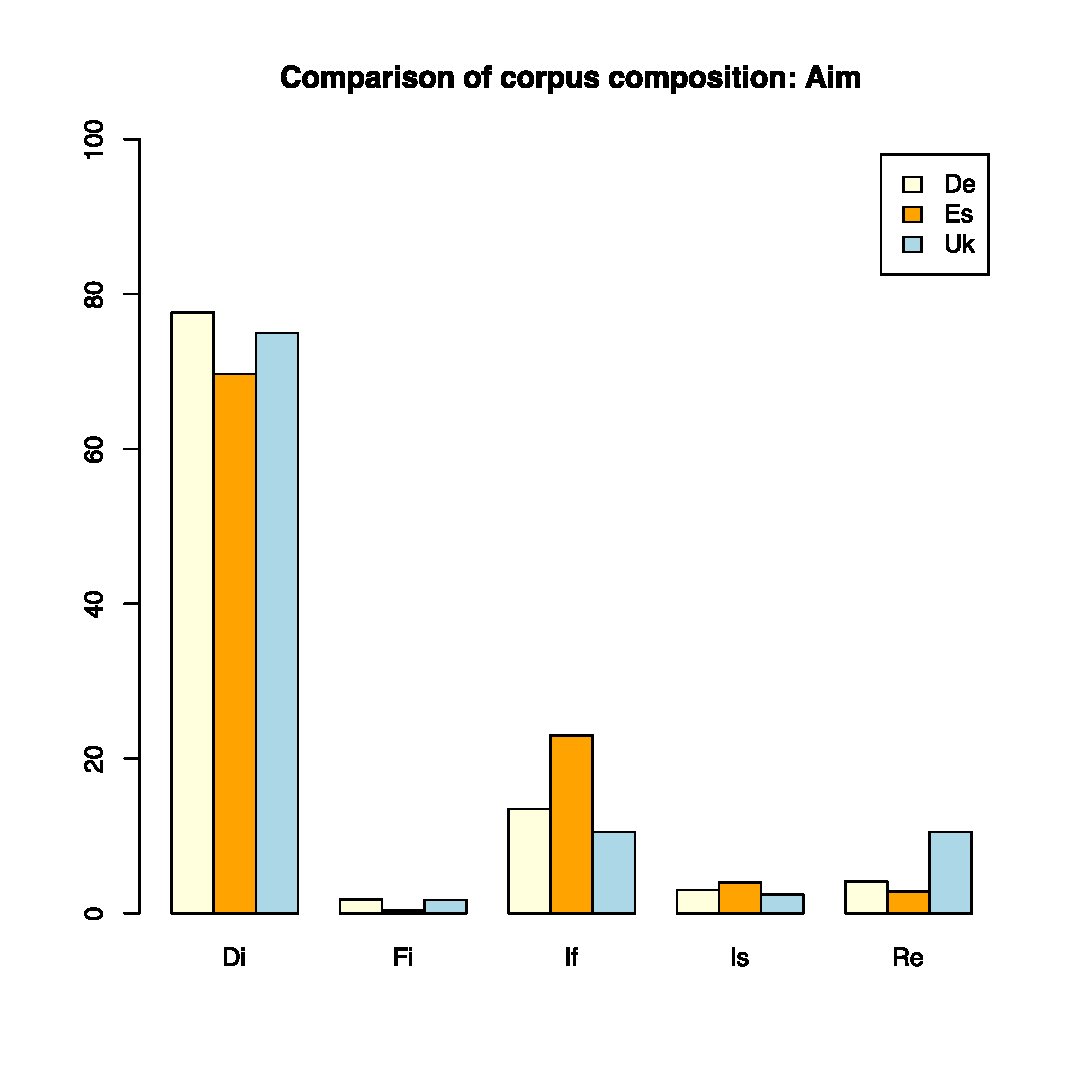
\includegraphics[width=0.65\textwidth]{graphics/aim}
\end{frame}

\begin{frame}
  {TLD-Vergleich}
  \centering
  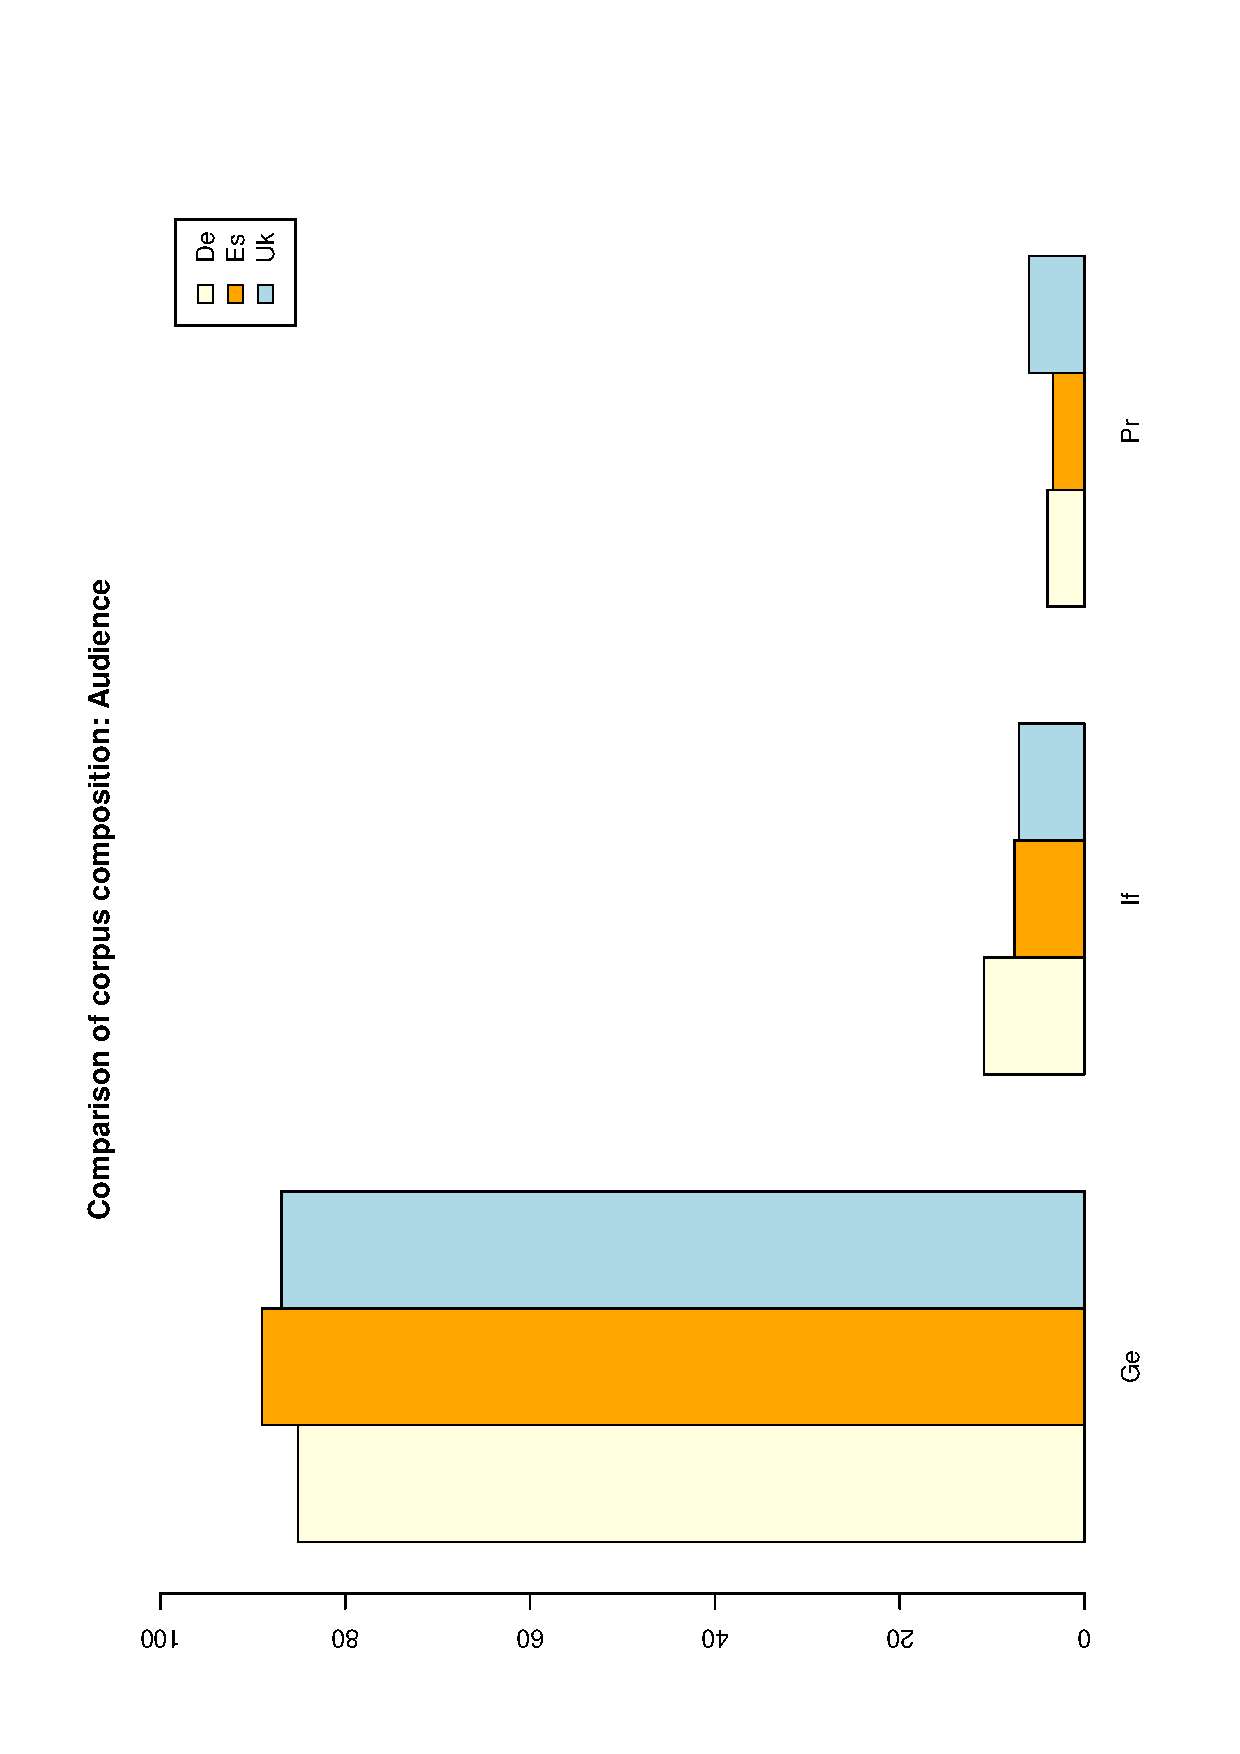
\includegraphics[height=0.95\textheight,angle=270]{graphics/aud}
\end{frame}

\begin{frame}
  {TLD-Vergleich}
  \centering
  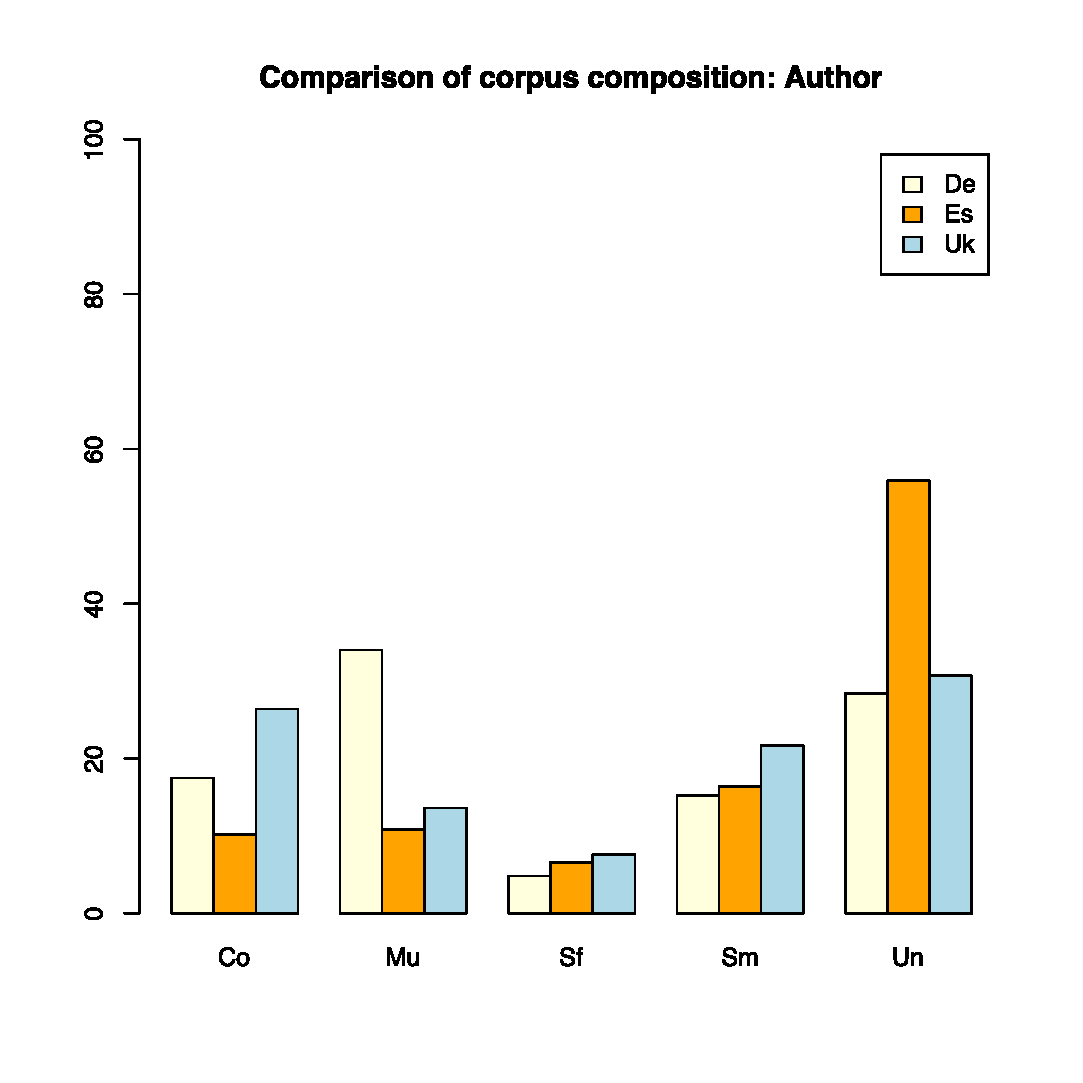
\includegraphics[width=0.65\textwidth]{graphics/aut}
\end{frame}

\begin{frame}
  {TLD-Vergleich}
  \centering
  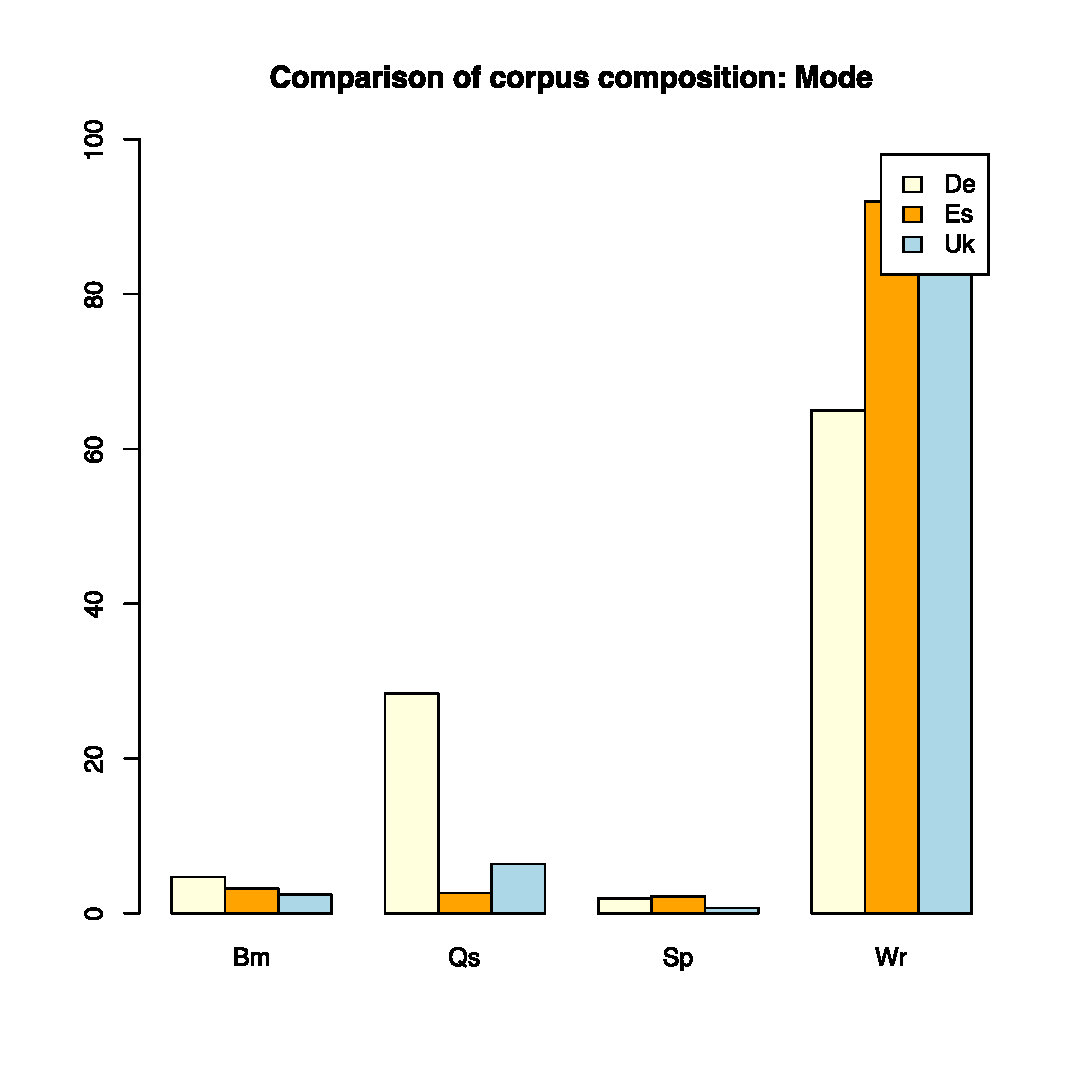
\includegraphics[width=0.65\textwidth]{graphics/mode}
\end{frame}


\include{include/distsem_en}
%\subsection{COCO: Die dritte Generation}

\begin{frame}
	{CommonCrawl}
	\begin{itemize}
	  \item sehr große Mengen von Crawldaten frei verfügbar
	  \item Sitz in USA, gedeckt durch Fair Use
	  \item archiviert unter Amazon Public Datasets-Programm
	  \item TB-weise über HTTP runterladbar (alternativ S3)
	\end{itemize}
\end{frame}


\begin{frame}
	{COCO: Common COW}
	\begin{itemize}
	  \item Daten-Derivate sind rechtlich unproblematisch
	  \item unsere eigentlich Leistung: \alert{Derivate}, also die Bereinigungen, Qualitätsmaße und Annotationen
	  \item Idee: \alert{Derivate von uns frei (CC-BY),\\Primärdaten von CommonCrawl}

	  \vspace{0.5cm}

	  \item Nebeneffekt: Massencrawling ist ein mühsames und\\gefährliches Unterfangen, wird dadurch gespart
	\end{itemize}
\end{frame}


\begin{frame}
	{COCO Arbeitsablauf}
	\centerinag
	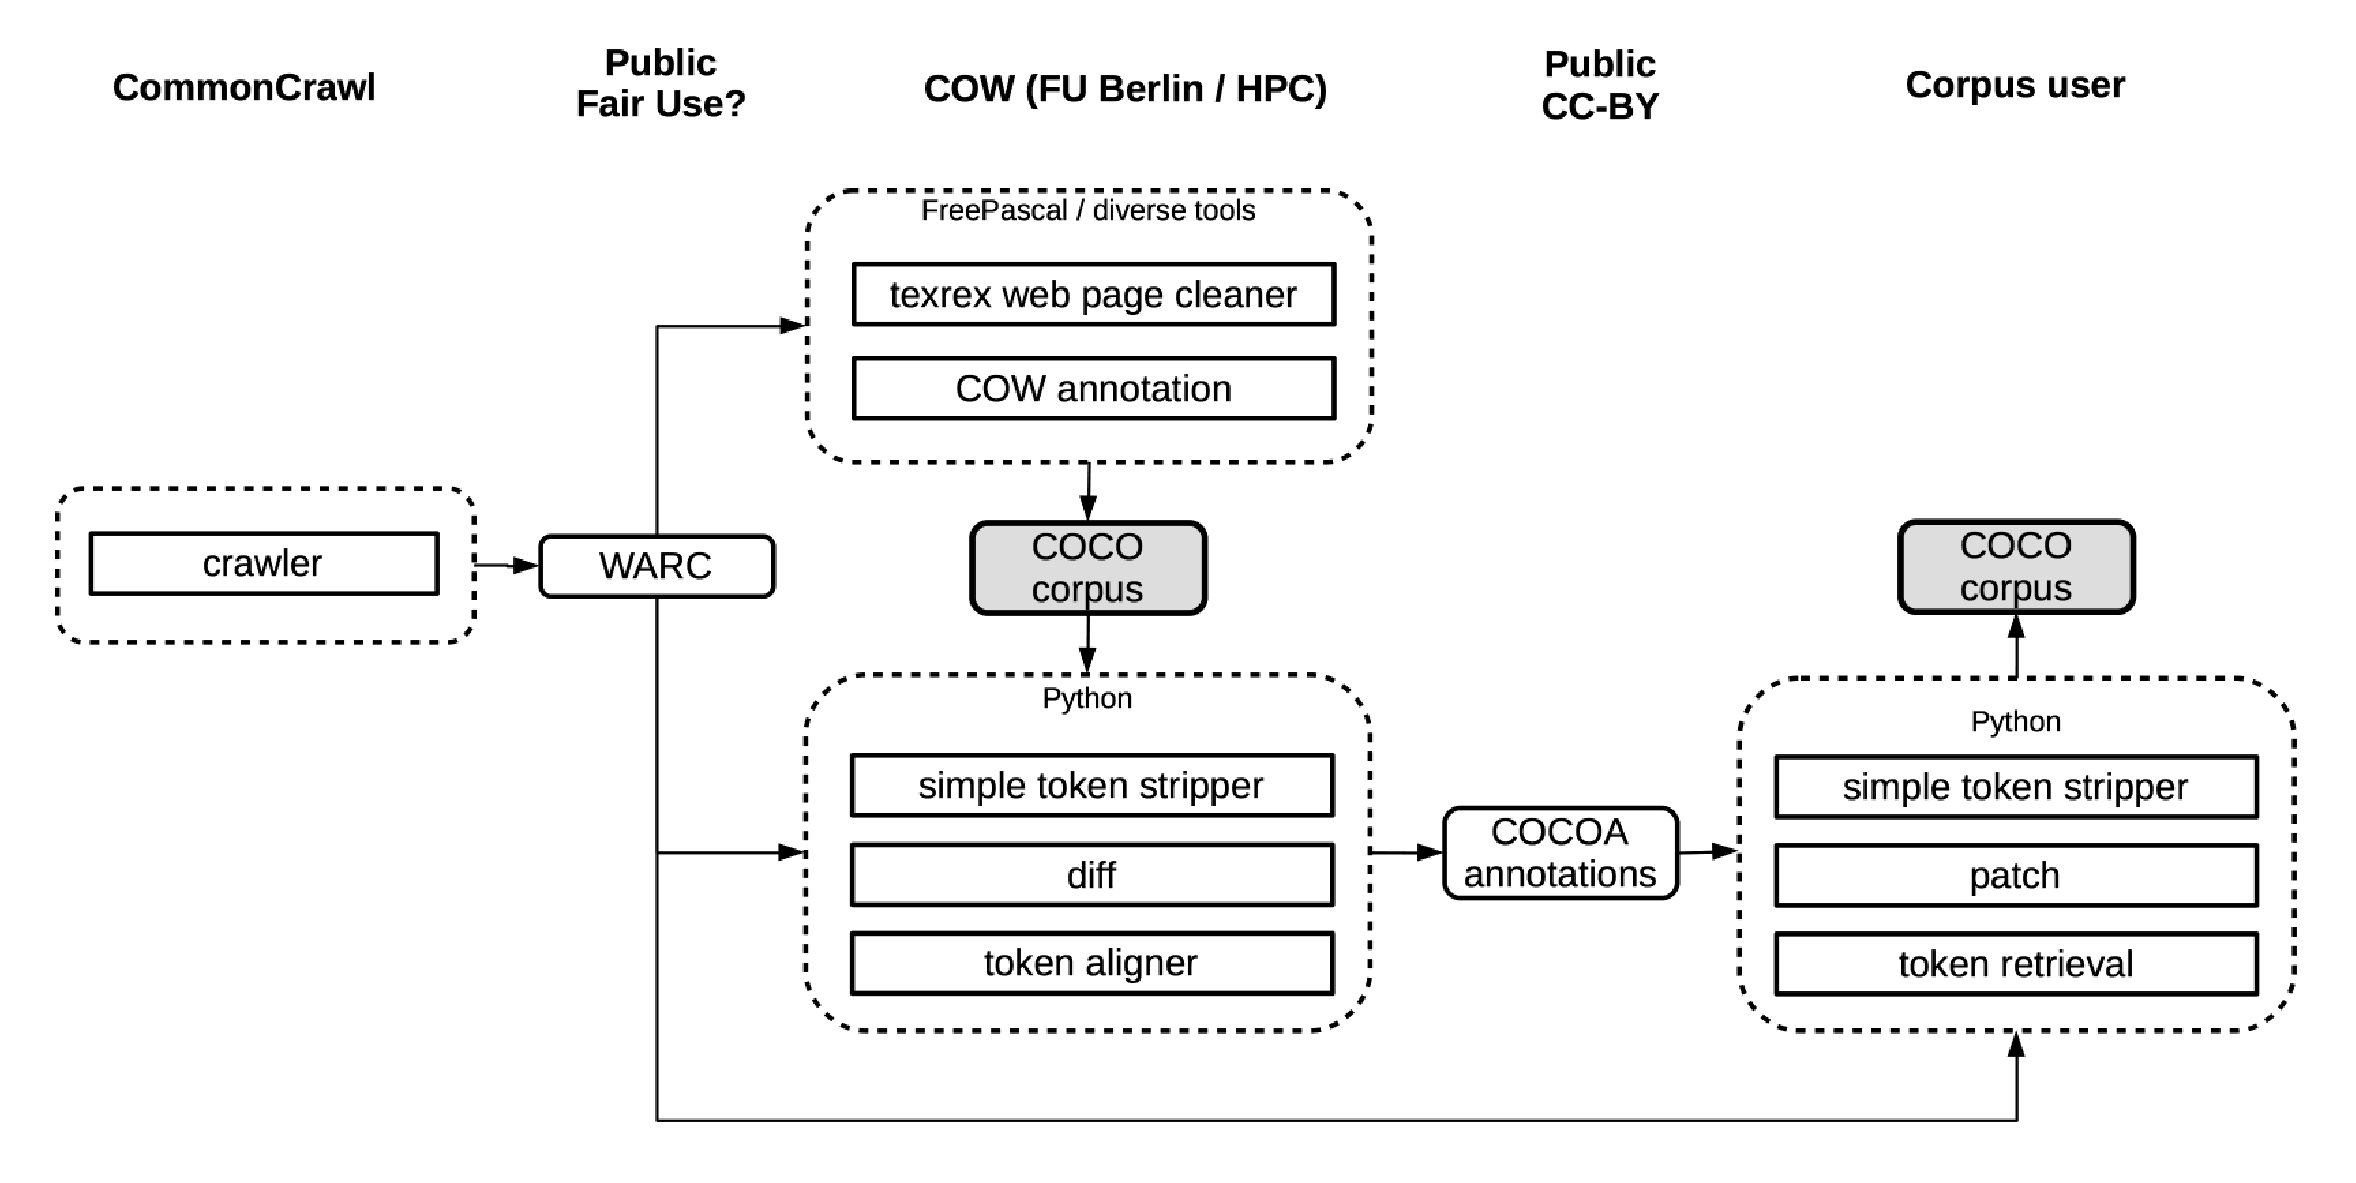
\includegraphics[width=0.9\textwidth]{graphics/workflow}
\end{frame}


\begin{frame}
	{Beispiel für COCOA-Datenformat}

	\centering
	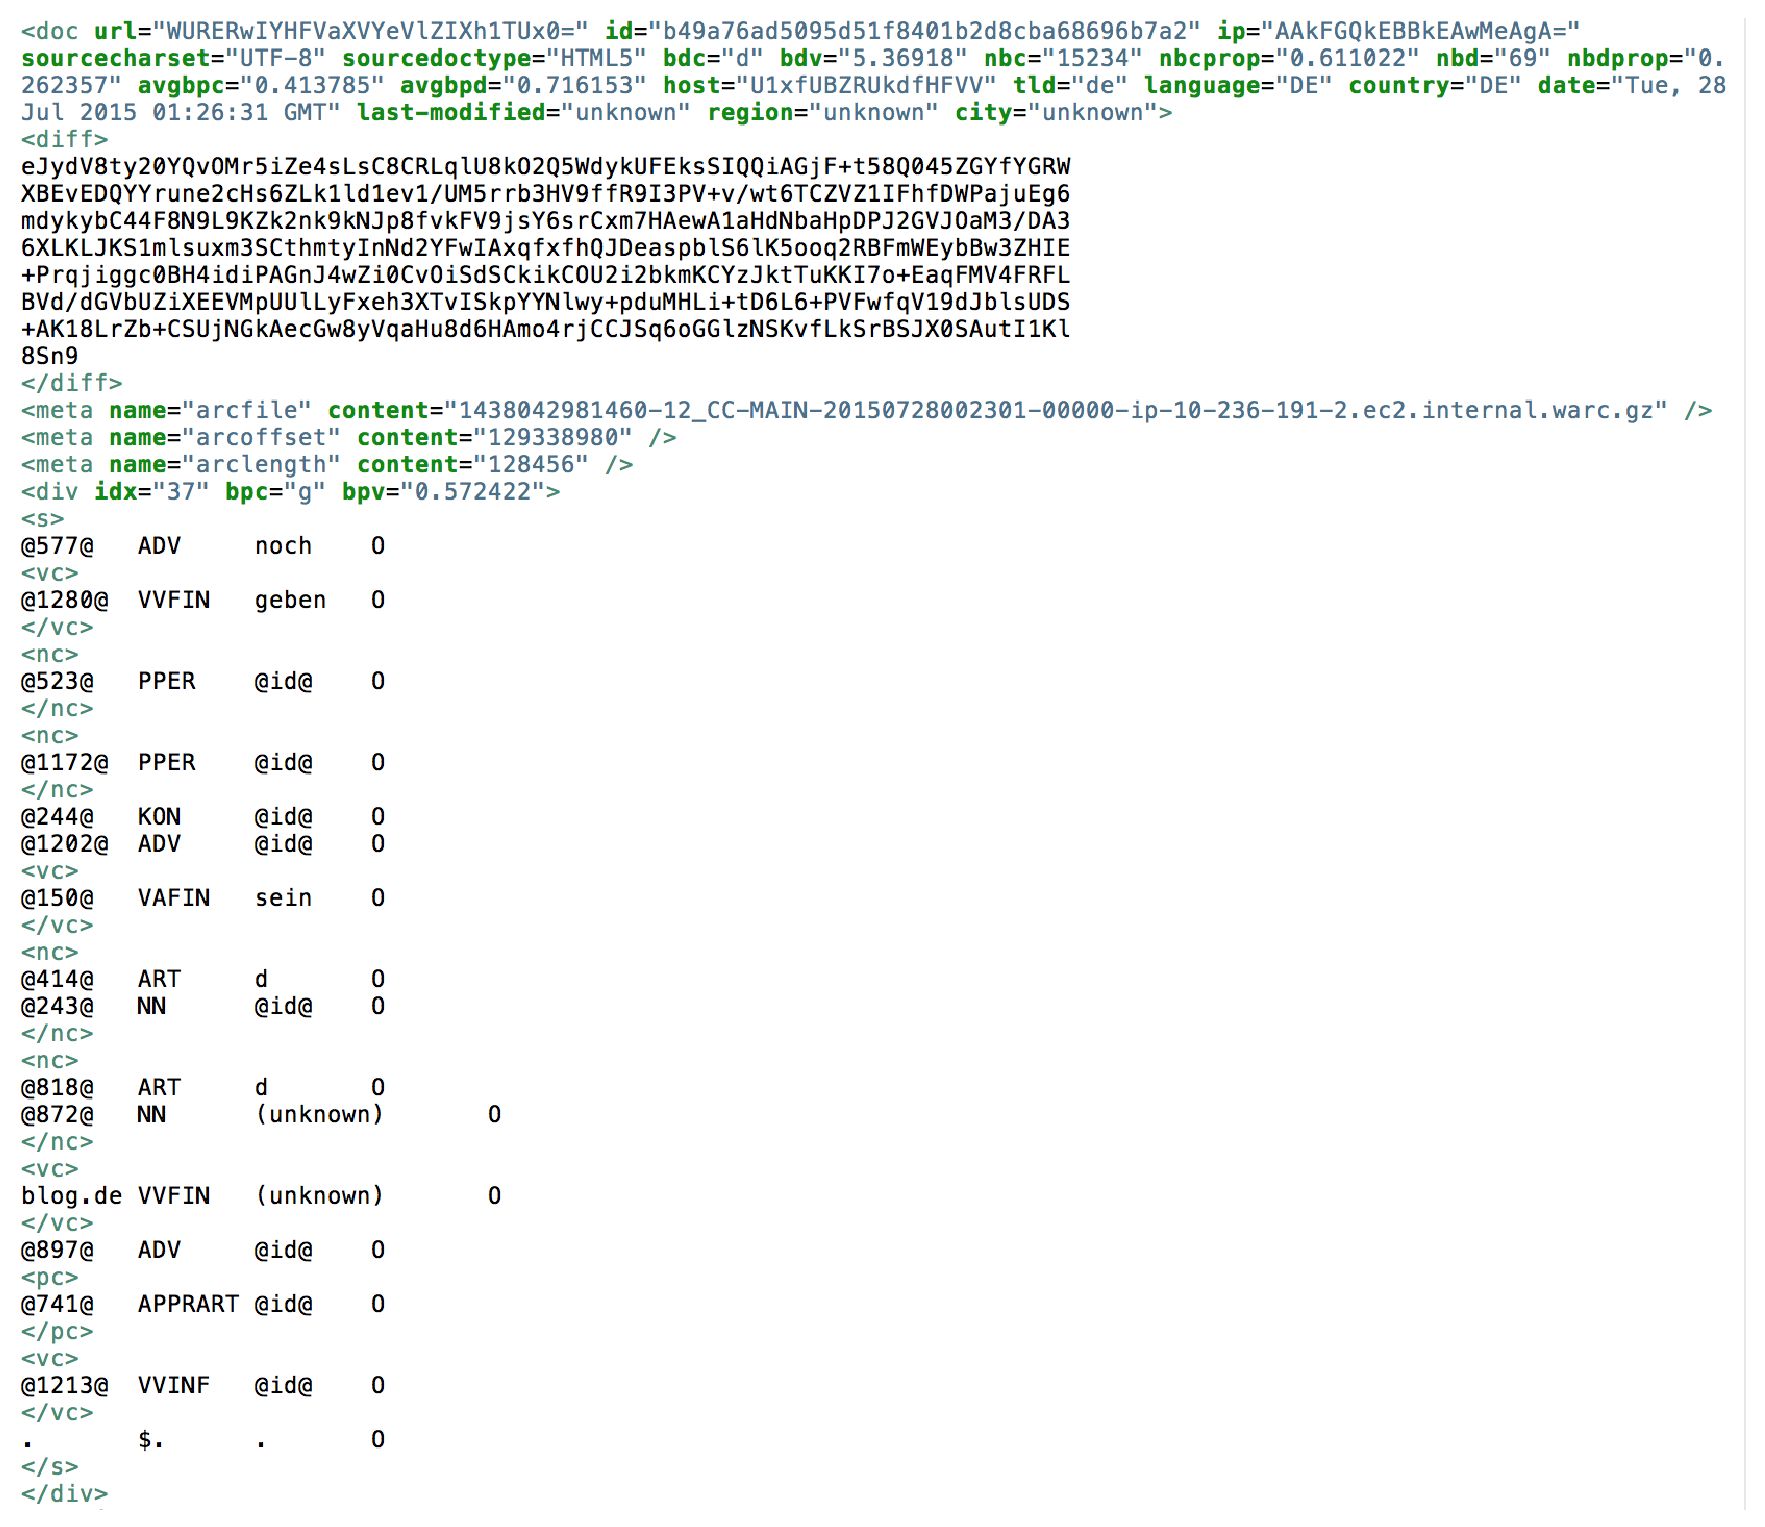
\includegraphics[height=0.85\textheight]{graphics/cocoa}
%	\scalebox{0.4}{\ttfamily
%	\begin{tabular}{llllll}
%		\hline
%		\multicolumn{6}{l}{<doc url="6ad87fe6a1b26920e1fd27eaf334" offset="92575231" length="12331">} \\
%		<s> &&&&& \\
%		<vc> &&&&& \\
%		@8702@5@  & VB   &   check  & 1  &    0    &   null \\
%		</vc> &&&&& \\
%		<nc> &&&&& \\
%		@8708@3@  &   DT    &  <id />   &  2  &     6  &     det \\
%		@8712@2@    &  NP     & <id />   &   3    &   6   &    poss \\
%		\&apos;s & POS  &   \&apos;s &4    &   3  &     possessive \\
%		</nc> &&&&& \\
%		<nc> &&&&& \\
%		@8718@7@ &NP   &   <id /> &5  &     6   &    nn \\
%		@8726@7@ &NN  &    <id /> &6      & 1   &    dobj \\
%		</nc> &&&&& \\
%		<advc> &&&&& \\
%		@8734@12@ &   RB   &   <id /> &   7   &    1    &   advmod \\
%		</advc> &&&&& \\
%		<pc> &&&&& \\
%		@8747@3@ &    IN    &  <id />  &   8   &    1   &    prep \\
%		<nc> &&&&& \\
%		@8751@7@ &NNS   &  update & 9   &    8     &  pobj \\
%		</nc> &&&&& \\
%		</pc> &&&&& \\
%		.     &  SENT  &  .   &    10  &    1   &    punct \\
%		</s> &&&&& \\
%		\hline
%	\end{tabular}}	
\end{frame}




\section{Recent developments}

%\subsection{ClaraX: Verzerrungsreduziertes Crawling}

\begin{frame}
  {Problem: Breadth-First-Search-Crawling}
  \begin{itemize}
    \item Crawling: neue Webseiten auf Basis der Links\\
      in bereits bekannten Webseiten finden
    \item Queueing-Strategie bestimmt Crawling-Algorithmus
    \item typisches BFS: alle Links in Reihenfolge des Auffindens queuen
      \vspace{0.5cm}
    \item BFS: bekannter nicht-korrigierbare Verzerrung\\
      abhängig vom \alert{Eingangsgrad}
  \end{itemize}
\end{frame}

\begin{frame}
  {Ist Verzerrung ein Problem?}
  \begin{itemize}
    \item je nach Anwendungsszenario\ldots
    \item für theoretische linguistische Fragestellungen,\\
      wie sie uns interessieren: \alert{Ja!}
    \item auch ohne Glauben an Balanciertheit/Repräsentativität:\\
      starke unbekannte Verzerrung macht \alert{nie} gute Stichproben
    \item vgl.\ SECOW11: 75\% aller Dokumente vom selben Bloghoster
      \vspace{0.5cm}
    \item wenigstens: Effekte aus Korpuszusammensetzung untersuchen:\\
      DFG \textit{Webcharakterisierung} (SCHA1619-1)
  \end{itemize}
\end{frame}

\begin{frame}
  {Lösung: Korrigierte Random Walks}
  \begin{itemize}
    \item Random Walks: Verzerrung nach \alert{PageRank}
    \item wenn PageRank bekannt oder schätzbar,\\
      Verzerrungskorrektur durch Rejection Sampling möglich
    \item verschiedene Methoden, unterschiedlich impraktibabel
    \item auf jeden Fall: maximal kleine Referenzkorpora: \alert{RandyCOW}
  \end{itemize}
\end{frame}

\begin{frame}
  {ClaraX}
  \begin{itemize}
    \item voll bemerkmalter Random Walker
    \item Politeness: voll, reduziert, gar nicht, stealth mode(s)
    \item Dead-end-Strategien: terminate, jump, backtrack
    \item scope restriction\slash black \& white list
    \item follow modes: same host, same virtual host, different host oder Kombinationen
    \item Verarbeitung eingebaut: Spracherkennung, Dokumentqualität, Boilerplate, etc. (texrex)
    \item praktisch Möglich: Einschränkung auf\\
      bestimmte \alert{Segmente} des WWW
  \end{itemize}
\end{frame}

\begin{frame}
  {Baseline-Experiment 1: True Random Walking}
  \begin{itemize}
    \item jedem Link folgen (auch intern)
    \item nur deutsche Dokumente (step back wenn nicht Deutsch)\\
      in \textit{at}, \textit{ch}, \textit{de}
    \item 12.75 Tage, 1 Millionen Schritte
    \item entdeckte Hosts: \alert{1,227}
    \item durchschnittliche Verweildauer auf Host: \alert{16.42} Schritte
    \item mittlere Anzahl Dokumente pro Host: \alert{890.83}
  \end{itemize}
\end{frame}

\begin{frame}
  {Baseline-Experiment 2: Host Walking}
  \begin{itemize}
    \item Ineffizienz von seitenweisem Random Walk: \alert{Host Walk}
    \item follow mode: different (virtual) host
    \item 25.36 Tage, 2.090.443 Schritte
    \item mittlere Anzahl Dokumente pro Host: \alert{10.25} (statt 890.83)
    \item Problem: aggressives Rejection Sampling braucht\\
      noch längere Walks
  \end{itemize}
\end{frame}

\begin{frame}
  {Effekt von aggressivem Rejection Sampling}
  Relativ zu einer \alert{gewünschten} Korpusgröße:\\
  \vspace{0.5cm}
  \centering
  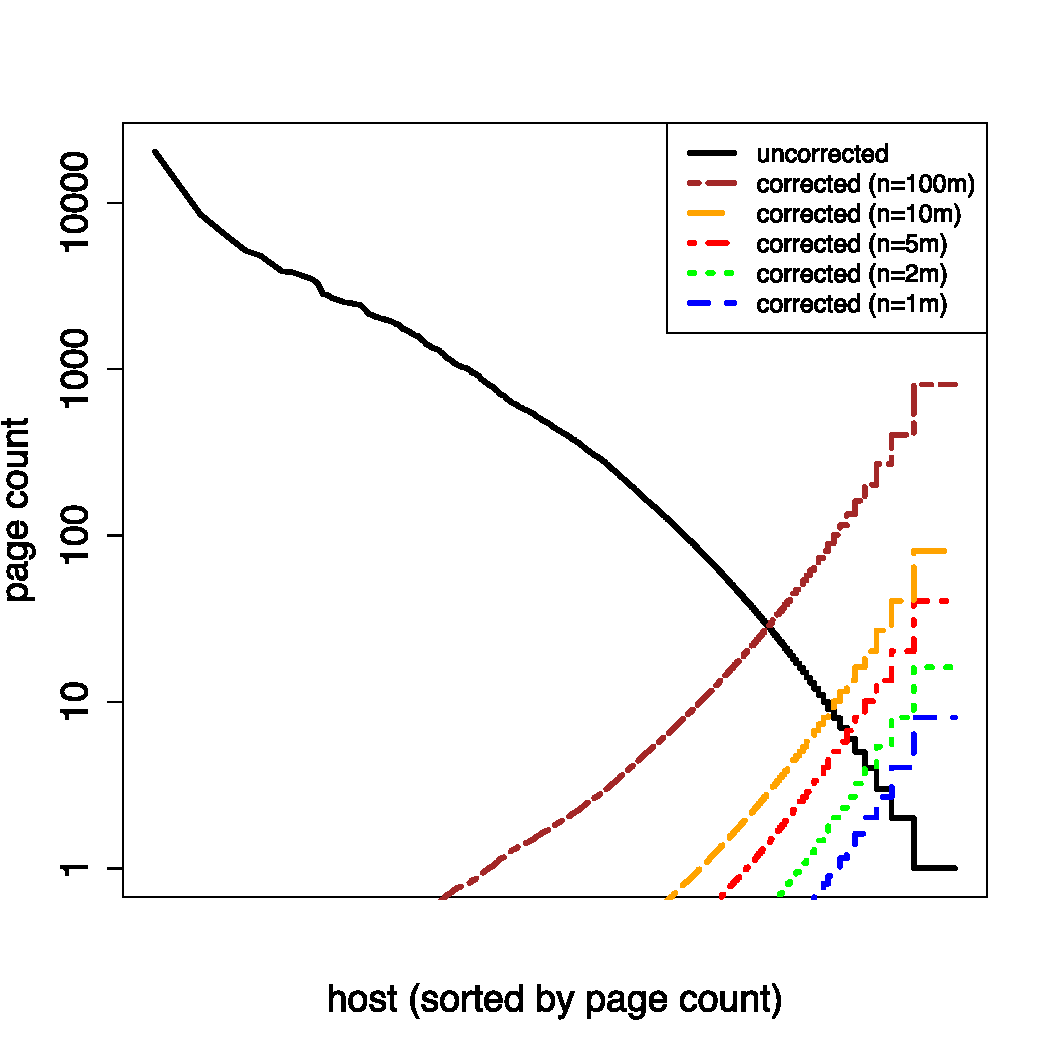
\includegraphics[width=0.5\textwidth]{graphics/corrected}\\
  \vspace{0.1cm}
  \pause
  \raggedright
  Was kann man da machen? \ldots
\end{frame}

%\subsection{Document classification (FU/DFG + IDS Grammatik)}

\begin{frame}
  {Goals of the classification}
  \begin{itemize}
    \item development of a data-driven approach
    \item taxonomy must be learnable well by automatic classifier\\
      (\alert{not} like Biber & Egbert 2016)
    \item large scale assessment of composition of web corpora,\\
      comparison DeReKo vs.\ DECOW
    \item generation of linguistically interpretable meta data
    \item two parts of the COReXiKO framework:\\
      \alert{class.\ by grammatical features} (COReX),\\
      \alert{class.\ by lexical distributions} (topic modeling: COReKo)
  \end{itemize}
\end{frame}

\begin{frame}
  {COReKo method}
  \begin{itemize}
    \item intended COWCat classification by \alert{topic domain}
    \item 20 categories (politics, sports, arts, etc.)
    \item two gold standards for DECOW and DeReKo 
    \item first step: \alert{topic modeling} (LSI, LDA)\\
      generates topic-document matrices (TDM)
    \item second step: \alert{supervised classification}\\
      of topic domains learned from TDM
  \end{itemize}
\end{frame}

\begin{frame}
  {Experiment COReKo 1}
  \begin{itemize}
    \item gold standard: ca.\ 800 documents from DECOW, DeReKo each
    \item topic modeling: GenSim (LSI. LDA)
    \item topic domain classifier: SVM
    \item diverse different processing options\\
      (usually best lemma+POS, use only content words)
    \item 20--90 topics
    \item incremental mix-in of non-gold standard document for topic modeling to increase stability of the topics
  \end{itemize}
\end{frame}

\begin{frame}
  {Results COReKo 1}
  Accuracy (10CV) DECOW\\
  \centering
  \vspace{0.5cm}
  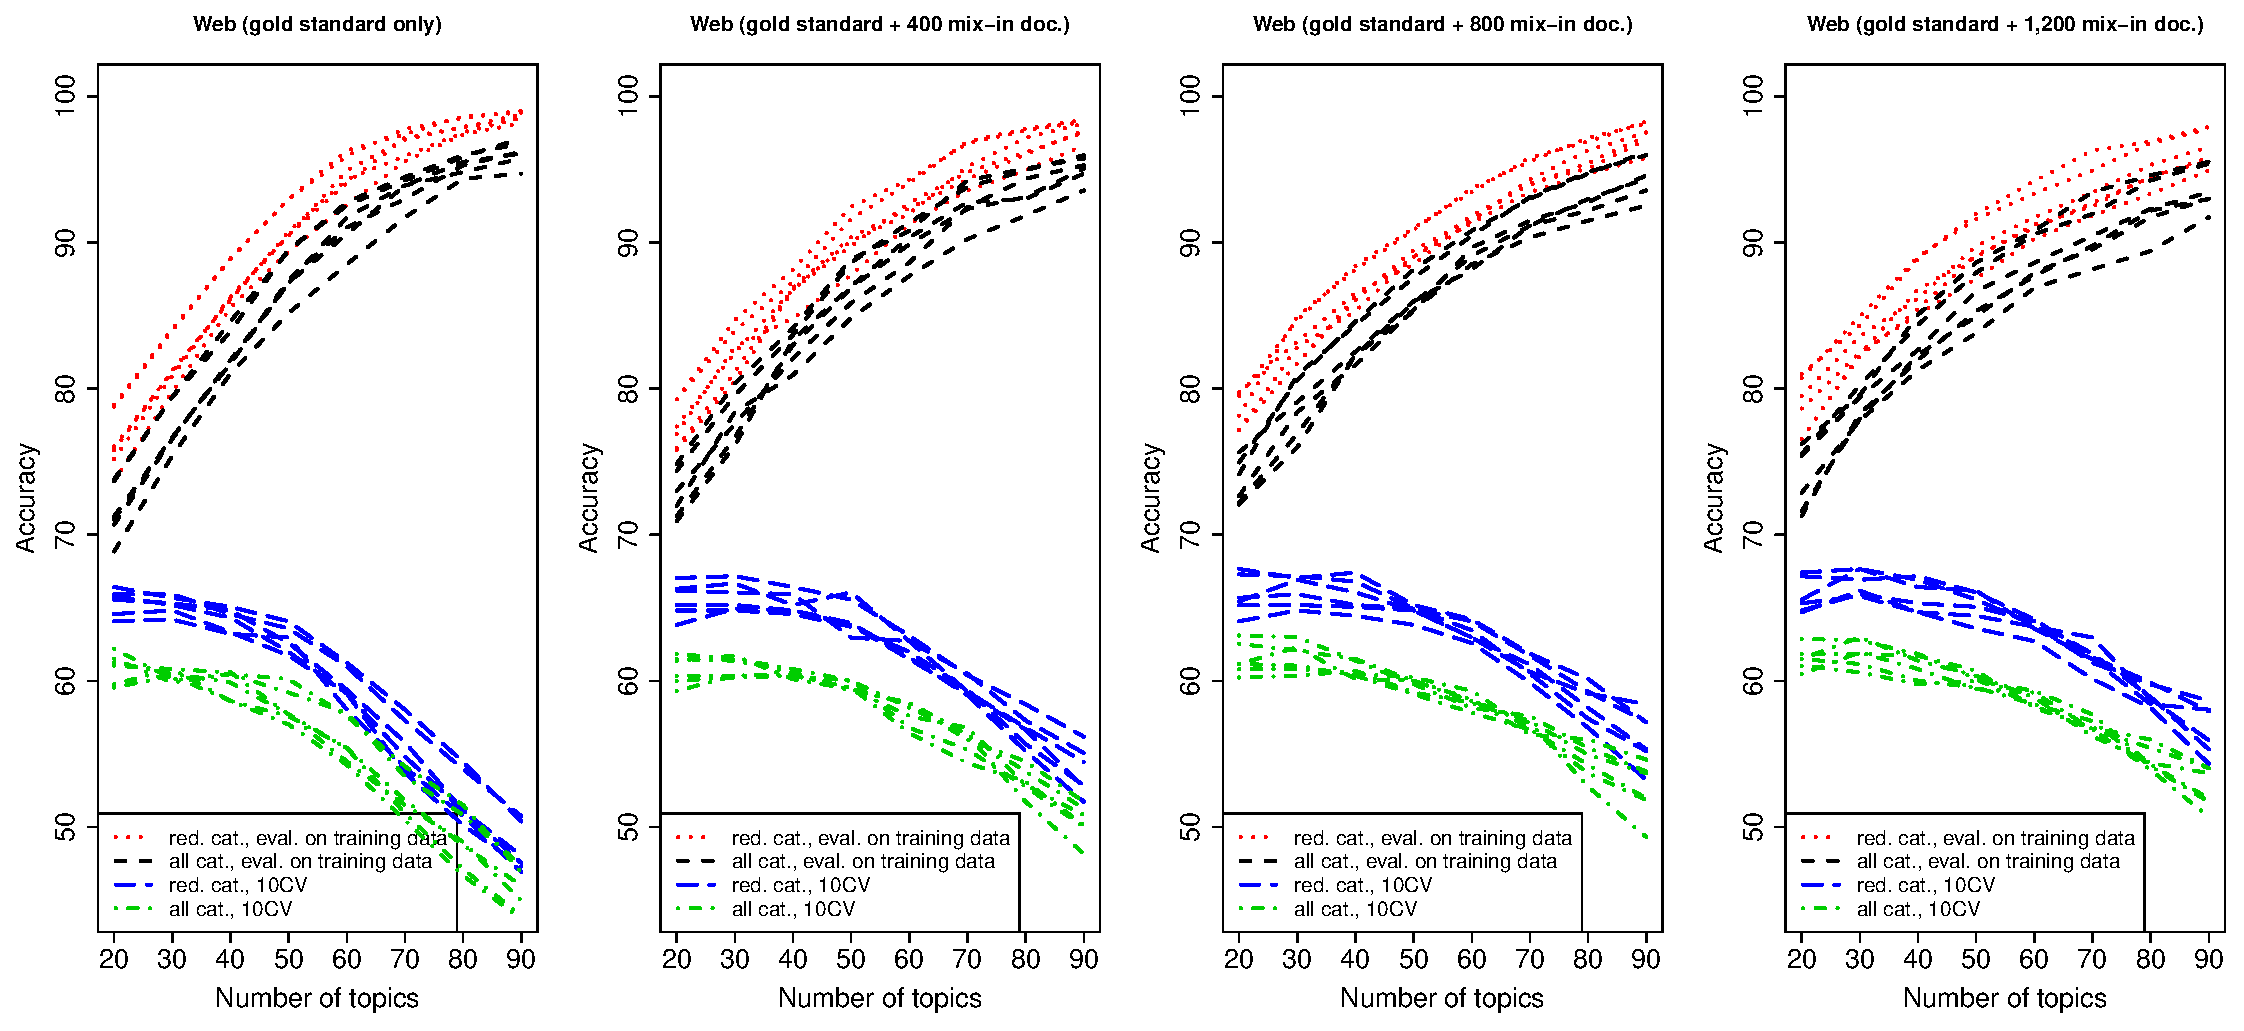
\includegraphics[width=0.8\textwidth]{graphics/cow}
\end{frame}

\begin{frame}
  {Results COReKo 1}
  Accuracy (10CV) DeReKo\\
  \centering
  \vspace{0.5cm}
  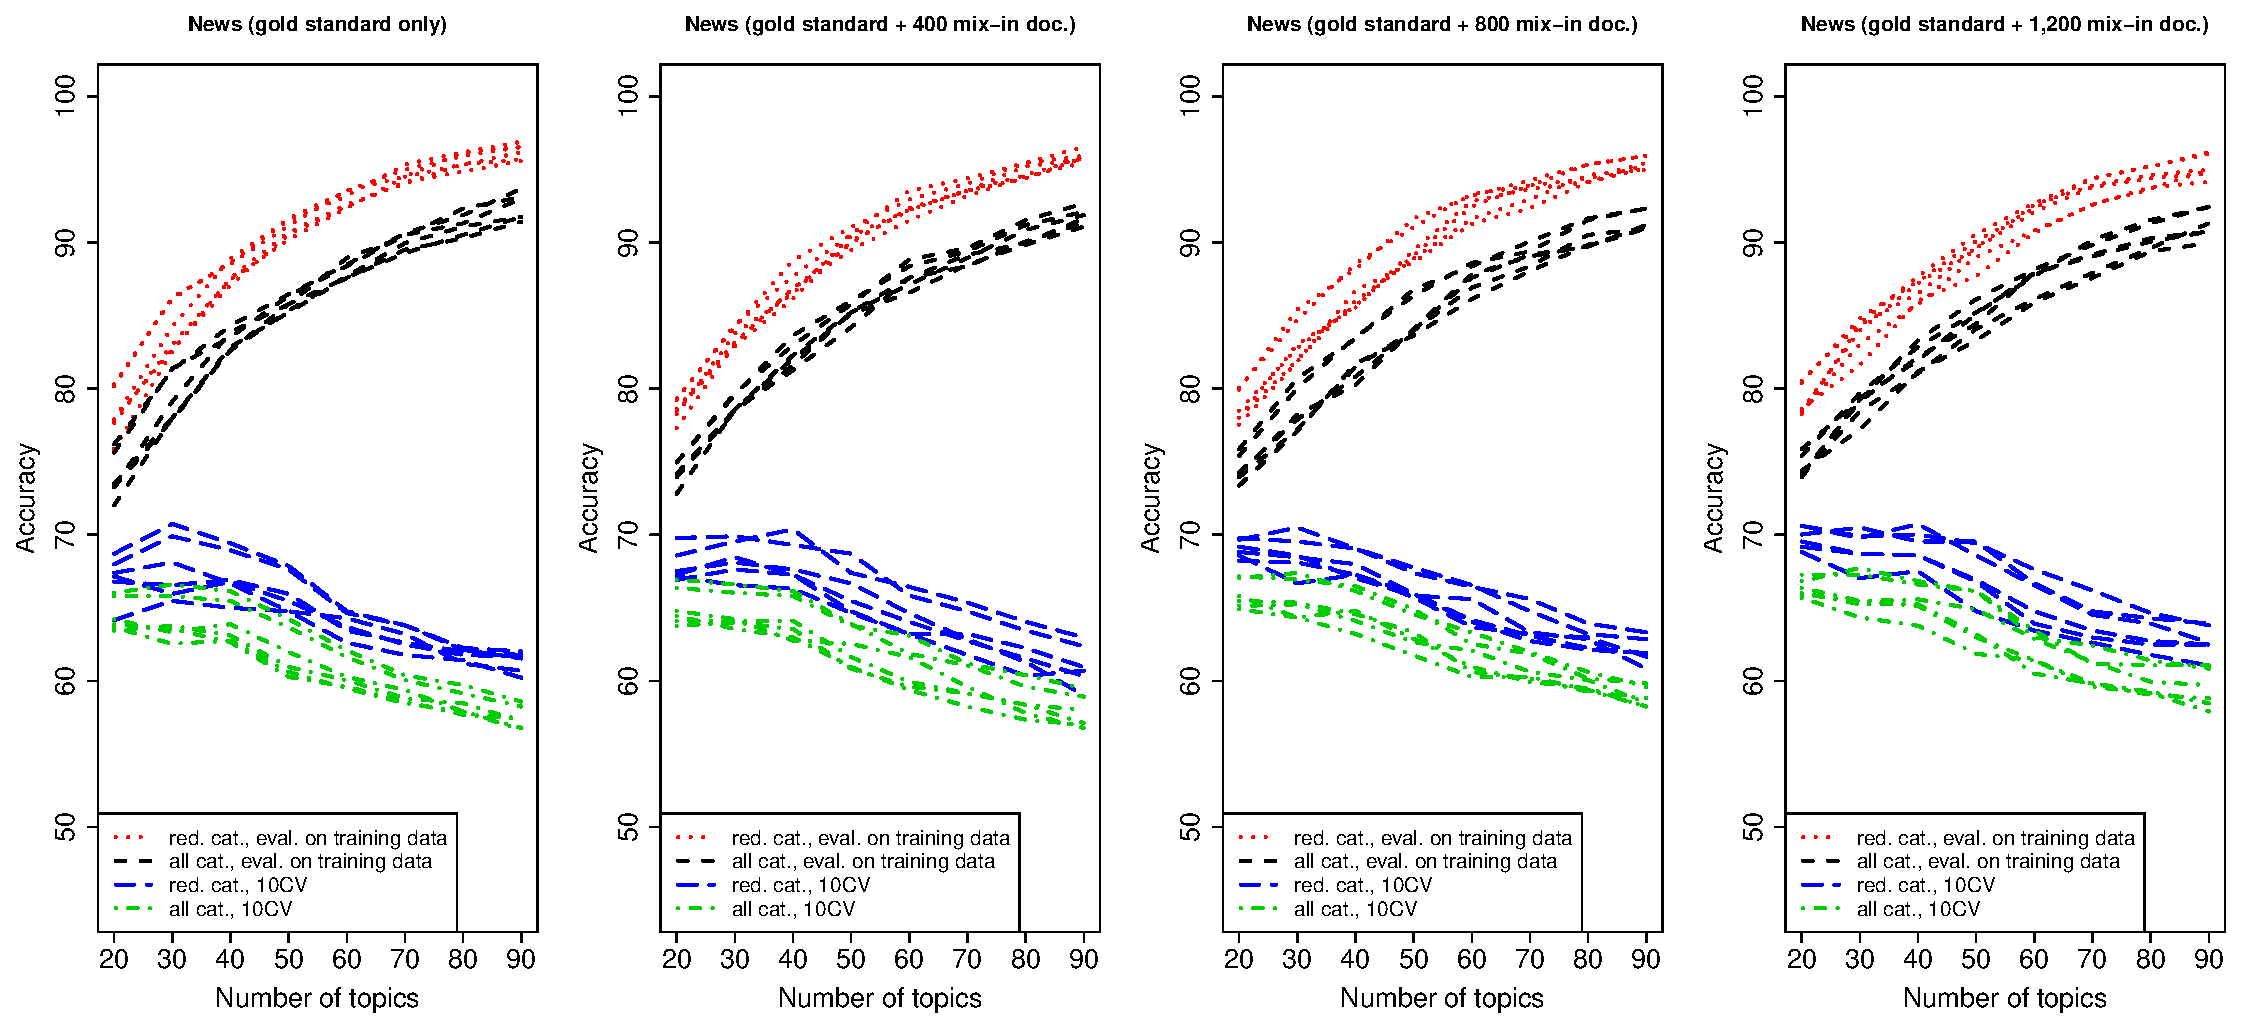
\includegraphics[width=0.8\textwidth]{graphics/dereko}
\end{frame}

\begin{frame}
  {Results COReKo 1}
  Accuracy (10CV) \alert{DECOW + DeReKo}\\
  \centering
  \vspace{0.5cm}
  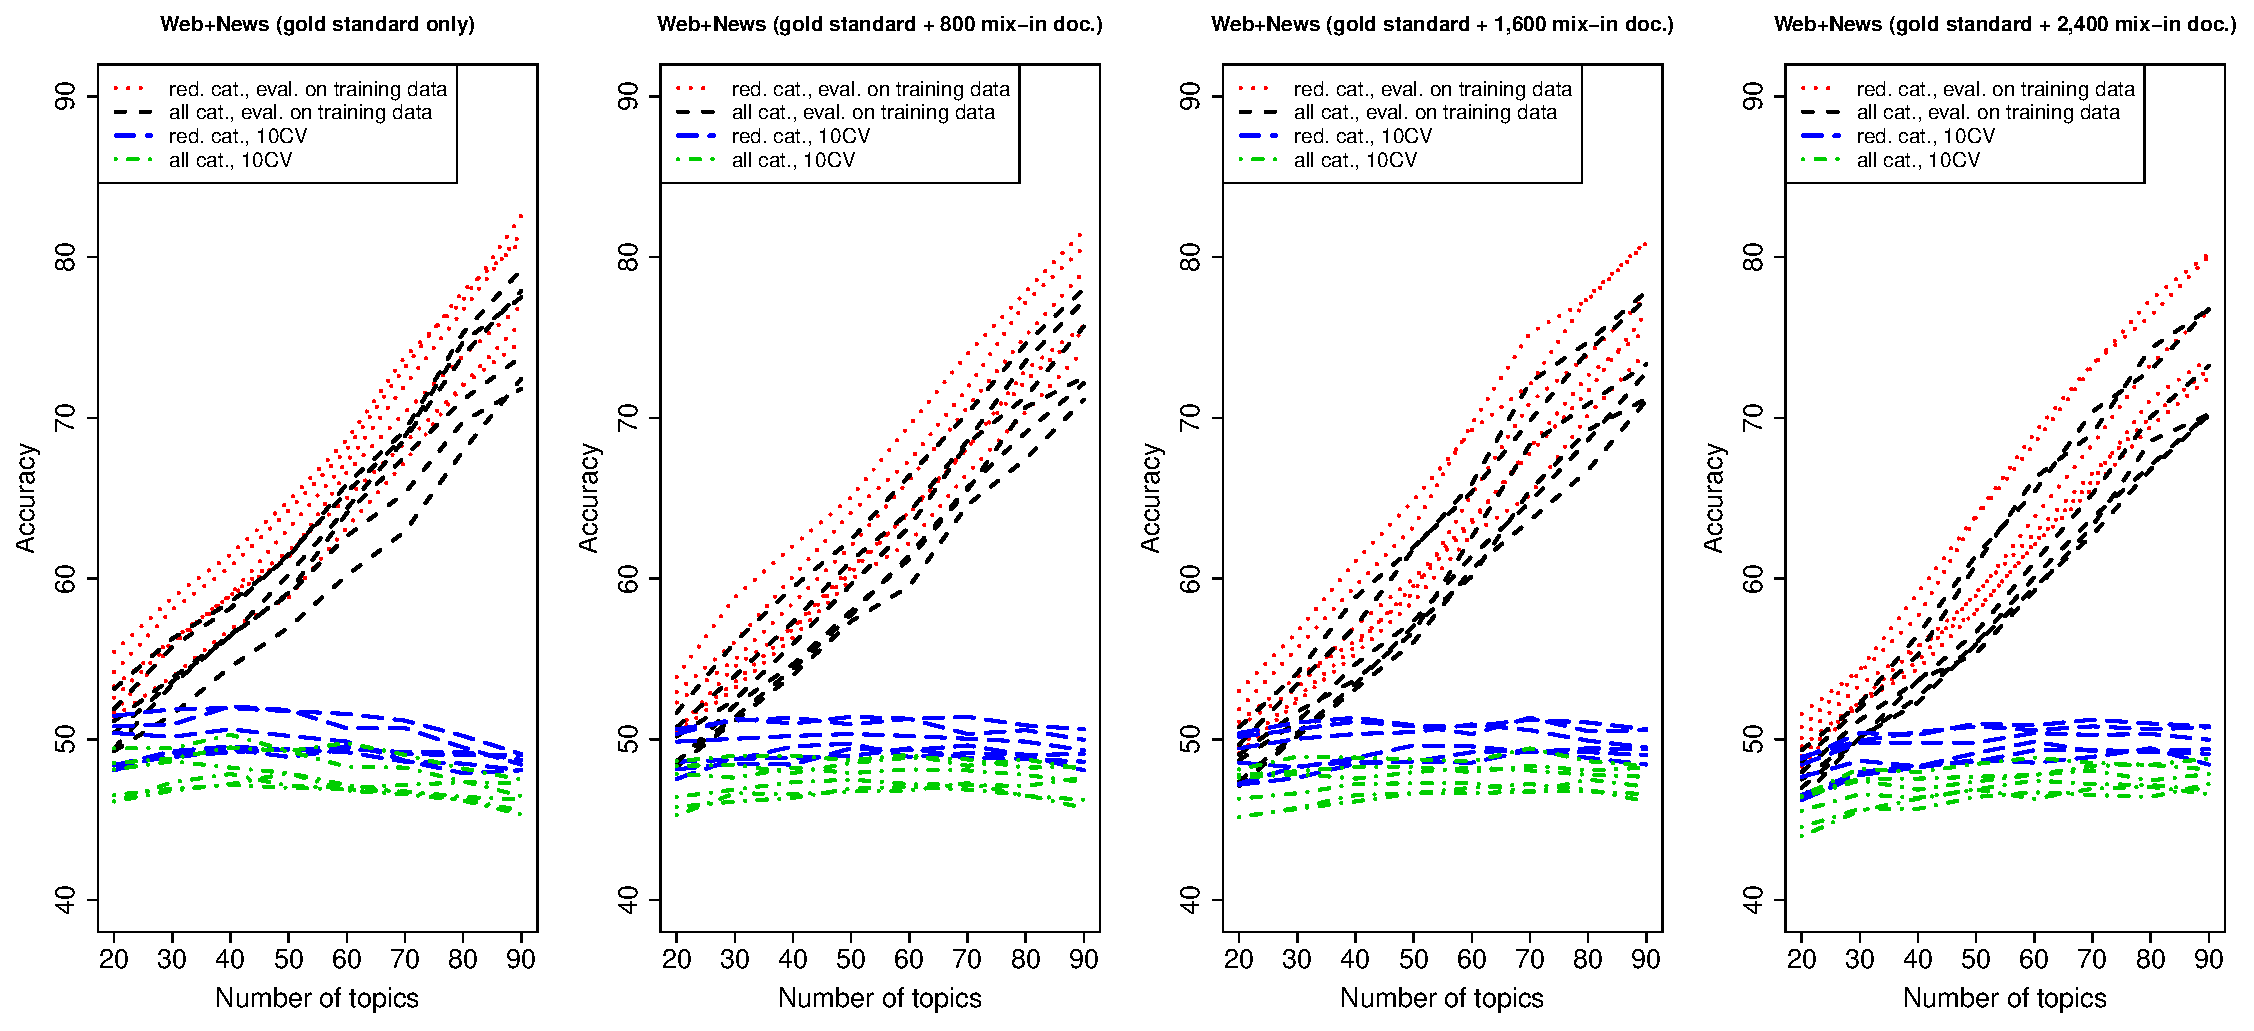
\includegraphics[width=0.8\textwidth]{graphics/coreko}
\end{frame}

\begin{frame}
  {Reasons for moderate quality}
  \centering
  \scalebox{0.55}{\begin{tabular}{|llcccccccc|}
    \hline
    %\multicolumn{2}{|c}{\textbf{COW}} & \multicolumn{8}{c|}{\textbf{Classified}} \\
    \multicolumn{2}{|c}{\textbf{Web}} & \multicolumn{8}{c|}{\textbf{Classified}} \\
     && \rot{\textbf{PolSoc~}} & \rot{\textbf{Busi}} & \rot{\textbf{Life}} & \rot{\textbf{Arts}} & \rot{\textbf{Public~}} & \rot{\textbf{Law}} & \rot{\textbf{Beliefs~}} & \rot{\textbf{Hist}} \\
   \hline
   \multirow{8}{*}{\rot{\textbf{Annotated}}} & \textbf{PolSoc}  & \textbf{26} &  12 &  10 &   1 &   1 &   0 &   1 &   0 \\ 
     & \textbf{Busi}    &  5 & \textbf{105} &  40 &   7 &   1 &   2 &   1 &   1 \\ 
     & \textbf{Life}    &  3 &  14 & \textbf{286} &   6 &   4 &   1 &   1 &   1 \\ 
     & \textbf{Arts}    &  3 &   2 &  36 &  \textbf{78} &   1 &   0 &   2 &   6 \\ 
     & \textbf{Public}  &  0 &   3 &  11 &   0 &   \textbf{9} &   1 &   0 &   0 \\ 
     & \textbf{Law}     &  3 &   9 &   8 &   0 &   1 &   \textbf{8} &   0 &   0 \\ 
     & \textbf{Beliefs} &  4 &   3 &  11 &   6 &   1 &   0 &  \textbf{30} &   1 \\ 
     & \textbf{Hist}    &  9 &   0 &   9 &   7 &   1 &   1 &   2 &  \textbf{15} \\ 
     \hline
   \end{tabular}}
\end{frame}
 
\begin{frame}
  {Reasons for moderate quality}
  \centering
 \scalebox{0.55}{\begin{tabular}{|llcccccc|}
    \hline
     %\multicolumn{2}{|c}{\textbf{DeReKo}} & \multicolumn{6}{c|}{\textbf{Classified}} \\
     \multicolumn{2}{|c}{\textbf{News}} & \multicolumn{6}{c|}{\textbf{Classified}} \\
     && \rot{\textbf{PolSoc~}} & \rot{\textbf{Busi}} & \rot{\textbf{Life}} & \rot{\textbf{Indiv}} & \rot{\textbf{Arts}} & \rot{\textbf{Public}} \\
    \hline
     \multirow{6}{*}{\rot{\textbf{Annotated}}}& \textbf{PolSoc}  & 223 & 6 & 39 &  0 &  0 &  8 \\
     & \textbf{Busi}    &  20 & 24 &   9 &  0 &  0 &  0 \\
     & \textbf{Life}    &  24 &  1 & 324 &  0 &  0 &  1 \\
     & \textbf{Indiv}   &   5 &  0 &  17 &  0 &  0 &  1 \\
     & \textbf{Arts}    &   2 &  0 &  28 &  0 &  6 &  0 \\
     & \textbf{Public}  &  35 &  0 &  30 &  0 &  0 & 34 \\
    \hline
  \end{tabular}}
\end{frame}
 
\begin{frame}
  {Reasons for moderate quality}
  \centering
\scalebox{0.55}{\begin{tabular}{|llccccccccc|}
    \hline
     \multicolumn{2}{|c}{\textbf{Pooled}} & \multicolumn{9}{c|}{\textbf{Classified}} \\
     && \rot{\textbf{PolSoc~}} & \rot{\textbf{Busi}} & \rot{\textbf{Med~}} & \rot{\textbf{Life}} & \rot{\textbf{Arts}} & \rot{\textbf{Public~}} & \rot{\textbf{Law}} & \rot{\textbf{Beliefs~}} & \rot{\textbf{Hist}} \\
    \hline
    \multirow{9}{*}{\rot{\textbf{Annotated}}} & \textbf{PolSoc}   & \textbf{199} &   7 &   0 & 109 &   0 &  12 &   0 &   0 &   0 \\ 
    & \textbf{Busi}     &  18 &  \textbf{23} &   0 & 172 &   0 &   2 &   0 &   0 &   0 \\ 
    & \textbf{Med}  &   6 &   0 &   \textbf{0} &  29 &   0 &   1 &   0 &   0 &   0 \\ 
    & \textbf{Life}     &  25 &   4 &   0 & \textbf{632} &   0 &   5 &   0 &   0 &   0 \\ 
    & \textbf{Arts}     &   2 &   2 &   0 & 160 &   \textbf{0} &   0 &   0 &   0 &   0 \\ 
    & \textbf{Public}   &  46 &   2 &   0 &  56 &   0 &  \textbf{19} &   0 &   0 &   0 \\ 
    & \textbf{Law}      &   8 &   0 &   0 &  31 &   0 &   0 &   \textbf{0} &   0 &   0 \\ 
    & \textbf{Beliefs}  &   0 &   0 &   0 &  59 &   0 &   0 &   0 &   \textbf{0} &   0 \\ 
    & \textbf{Hist}     &   4 &   0 &   0 &  50 &   0 &   0 &   0 &   0 &   \textbf{0} \\ 
    \hline
 \end{tabular}}
\end{frame}

\begin{frame}
  {CoReKO 2}
  \begin{itemize}
    \item larger gold standards (4000 documents each)
    \item improved classification scheme
    \item allow gradual multi-assignment
    \item allow virtually unclassified documents
    \item also: raw topic distributions as meta data
  \end{itemize}
\end{frame}



%\section{Anwendungen von COW Korpora}
%
%\begin{frame}
  {Publikationen mit COW-Daten}
  \begin{itemize}
    \item bekannt: 19 publizierte oder angenommene\\qualitätsgesicherte Artikel seit 2014 
    \item \url{http://corporafromtheweb.org/research-with-cow/}
    \item vermutlich hohe Dunkelziffer, vor allem bei Computerlinguisten
    \item im Folgenden: vier Studien von uns,\\eingereicht oder kurz davor 
  \end{itemize}
\end{frame}


%%\documentclass{beamer}
%\usepackage{etex}
%\usepackage[utf8]{inputenc}
%\usepackage[OT1]{fontenc}
%\usepackage[ngerman]{babel}
%%\usepackage[utf8x]{inputenc}
%\usepackage{colortbl}
%\usepackage{uzk}
%\usepackage{natbib}
%\usepackage{my-gb4e-slides}
%%\usepackage{felix-gb4e-slides}
%\usepackage{verbatim}
%\usepackage{url}
%\usepackage{bbding}
%\usepackage{amssymb}
%\usepackage{amsmath}
%
%\newcommand{\done}{\cellcolor{teal}done}  %{0.9}
%\newcommand{\hcyan}[1]{{\color{teal} #1}}
%
%%\definecolor{beamer@fuorange}{rgb}{.9,0.5,0.1}
%\definecolor{beamer@fuorange}{rgb}{.8,.3,0}
%\definecolor{beamer@fudarkgreen}{rgb}{0,0.4,0}
%\definecolor{Gray}{gray}{0.5}
%\definecolor{Black}{gray}{0}
%\setbeamercolor{alerted text}{fg=beamer@fuorange}
%
%\let\citew=\citealp
%
%\newcommand{\cites}[1]{\citeauthor{#1}'s \citeyearpar{#1}}
\newcommand{\bluecell}{\cellcolor[rgb]{.7,.7,.9}}
\newcommand{\bluerow}{\rowcolor[rgb]{.7,.7,.9}}
\newcommand{\bluecol}{\columncolor[rgb]{.7,.7,.9}}
%\newcounter{lastpagemainpart}
%\setcounter{tocdepth}{1}
%
%\newcommand{\xxx}{\hspaceThis{[}}
%\newcommand{\Lf}{
%  \setlength{\itemsep}{1pt}
%  \setlength{\parskip}{0pt}
%  \setlength{\parsep}{0pt}
%}
%\newcommand{\graw}[1]{{\color[rgb]{0.5,0.5,0.5}#1}}
%\newcommand{\blaw}[1]{{\color[rgb]{0.2,0.2,0.9}#1}}
%\newcommand{\grien}[1]{{\color[rgb]{0.1,0.6,0.1}#1}}
%\newcommand{\myalert}[2]{{\color<#1>[rgb]{0,0.7,0}#2}}
%\newcommand{\eg}{e.\,g.}
%\newcommand{\Eg}{E.\,g.}
%\newcommand{\ie}{i.\,e.}
%\newcommand{\Ie}{I.\,e.}
%\newcommand{\Dim}{\cellcolor{Gray}}
%\newcommand{\Off}{\cellcolor{Black}}
%
%
%
%\begin{document}

% Includes hier! --------------------------------

\subsection{VSO in Spanish}

%\begin{frame}
%Fallstudie: VSO-Strukturen im Spanischen\\
%
%\footnotesize{gefördert von SFB 632/Informationsstruktur} 	
%\end{frame}

\begin{frame}
  \frametitle{VSO in Spanish}

Neutrale, unmarkierte Konstituentenabfolge im Spanischen: \textbf{SVO}\\[.3ex]
{\footnotesize (Contreras 1976; Hernanz \& Brucart 1987;
  Meirama 1997; Delbecque 2005; Gutierrez 2006, u.\,v.\,a.)}

\pause

\begin{itemize}
  \item[$\rightarrow$] Aber: je nach Verb/Verbklasse auch \textbf{VS} und \textbf{OVS}
\end{itemize}

\vspace{.5cm}

\pause

Andere Abfolgen sind nicht neutral/unmarkiert, sondern informationsstrukturell eingeschränkt

\begin{itemize}
  \item[$\rightarrow$] Oft beschrieben: \textbf{VOS} und \textbf{SV}
\end{itemize}

\vspace{.5cm}
 
\pause

Weniger oft beschrieben und immer noch ein wenig rätselhaft: \textbf{VSO}




\end{frame}


\begin{frame}
  \frametitle{VSO}


\begin{exe}
  \ex{[Buscaron]$_V$ [los padres]$_S$ [a la niña]$_O$ llenos de dolor sin encontrarla por ningún lado.}\\
    {\footnotesize `Voller Schmerz suchten die Eltern das Mädchen überall, ohne sie zu finden.'}

  \ex{[Deja]$_V$ [Di Stéfano]$_S$ [la dirección técnica]$_O$ y llega Amancio para dirigir al equipo.}\\
  {\footnotesize `Di Stéfano verlässt den Trainerposten und es kommt Amancio um die Mannschaft zu führen.'}
  
  \ex{[Posee]$_V$ [Huelva]$_S$ [unas increíbles playas de arena blanca]$_O$ \ldots}\  
      {\footnotesize `Huelva besitzt einige unglaubliche Strände mit weißem Sand'}
\end{exe}
\end{frame}


\begin{frame}
  \frametitle{VSO}\begin{itemize}
%\item relativ selten% 7--15\% deklarativer Hauptsätze in gesprochener
%  Sprache (berichtet in \citealp{Suner1982})
\item abhängig von der Textsorte (Gonzales de Serralde 2001)
\item abhängig von der regionalen Varietät\\ (z.\,B.\ nicht im mexikanischen
  Spanisch, Gutierrez 2006)
\item tritt \textit{nicht} in eng verwandten Sprachen auf, z.\,B.\ Katalanisch (Leonetti 2014), Italienisch (Belletti 2001)% im  frühen 19.\ Jhd.\ aber noch möglich, cf.\ \citealp{Wandruszka1982})
\end{itemize}
  
\end{frame}



\begin{frame}
  \frametitle{Eigenschaften von VSO}
  Einige intuitive/spekulative Beschreibungen, wenig empirisch fundiertes.\\[1ex]
  \centering
  \scalebox{.5}{  
\begin{tabular}{|p{3cm}|p{2cm}|p{2cm}|p{2cm}|p{2cm}|p{2cm}|}
\hline
                               & Suner (1982)      & Neumann-Holzschuh (1997) &  Zubizarreta (1998)  & Ordonez (2000) & Leonetti (2014)\\
\hline
Satzfokus                      &   \grien{\Checkmark}  & \alert{\XSolidBrush}        & \grien{\Checkmark}       & \grien{\Checkmark} & \grien{\Checkmark}\\
\hline
Subjekt im Fokus               &   \grien{\Checkmark}  
                                   (kontrastiv)        & \alert{\XSolidBrush}        &\grien{\Checkmark}
                                                                                       (kontrastiv)
                                                                                                                &\grien{\Checkmark} & \alert{\XSolidBrush}\\
\hline
Subjekt + Objekt im Fokus      &                       & \alert{\XSolidBrush}        &                          & \grien{\Checkmark} & \grien{\Checkmark}\\
\hline
\bluerow eine (einzige) Informationseinheit  &                  &   \alert{\XSolidBrush}      &                          &                   & \grien{\Checkmark}\\
\hline
\bluerow mehrere Informationseinheiten  &                       &  \grien{\Checkmark}         &                          &                   &\alert{\XSolidBrush}\\
\hline
Reihung von Ereignissen        &   \grien{\Checkmark}  &                             &                          &                  &  \\
\hline
Subjekt immer Teil
 der ``Assertion''             &                       &                             &                          & \grien{\Checkmark} & \grien{\Checkmark}\\
\hline
Subjekt gegeben                &                       &  \grien{\Checkmark}         &                          &                   &  \\
\hline
\end{tabular}
}
 
\end{frame}
\begin{frame}
\frametitle{Informationsstruktureller Status}

Es gibt fundamental verschiedene Annahmen über den informationsstrukturellen Status von \textbf{VSO}.\\[.3cm]


Neumann-Holzschuh (1997), empirische Studie:\\
\begin{itemize}
%\item ``markierte Variante'' kategorischer (rumnänisch)
\item kategorische Äußerung (Thema/Rhema-Gliederung)
\item Subjekt ist diskursgegeben und Thema
%\item beantwort die Frage: ``Und was geschah dann mit der gennannten Person/Sache?''
\item ``narrative Konstruktion'': zeigt \textit{topic-continuity} an
\end{itemize}

\pause
\vspace{.2cm}

Leonetti (2014), ``theoretische'' Überlegungen\\
(als ``Korpusstudie'' getarnt): 

 \begin{itemize}
  \item nur thetische Interpretation, keine informationsstrukturelle Gliederung
 \end{itemize}

\end{frame}


\begin{frame}
\frametitle{Frage}

Ist VSO eine Strategie zur ``De-Topikalisierung''?

    \begin{itemize}
    \item Das Subjekt wird aus der kanonischen Topikposition herausgenommen.
    \item Entsteht dabei eine Struktur, die als wide-focus/thetisch/event-reporting zu interpretieren ist?
    \end{itemize}
	
\end{frame}


\begin{frame}
 \frametitle{VSO: informationsstrukturell gegliedert oder nicht?}

Definition: ``thetisch'' 
\begin{quote}
   A thetic statement is uttered only if the elements that would constitute the predication base and the predicate in a corresponding categorical statement both convey (textually) new information.
\end{quote} (Sasse 1987: 567)

\pause
\vspace{.2cm}

Wenn VSO-Sätze thetisch sind, dann sind hier weniger diskursgegebene Subjekte zu erwarten, als bei SVO.

\end{frame}



\begin{frame}
  \frametitle{Korpusstudie (ESCOW12; 1,6 GT)}
  
  \begin{itemize}
    \item $N=20,000$ Verb-initiale Sätze   
    \item manuell VSO Strukturen herausfiltern:\\
      \begin{itemize}
      \item ``O'' ist direktes oder indirektes Objekt
      \item ``O'' ist eine NP oder PP (aber keine infinite VP oder Objektsatz)
      \end{itemize}
\end{itemize}
\pause

``Gesäuberte'' Stichprobe: 78 Belege ($0.4\%$) für VSO

\begin{itemize}
    \item Annotation von Diskursgegebenheit von Subjekt und Objekt\\
          (RefLex-Schema, Riester et al. 2010)
  \end{itemize}
\end{frame}

\begin{frame}
  \frametitle{Vergleich mit SVO}

$\rightarrow$ ``entsprechende'' Stichprobe von SVO-Sätzen.  

  \begin{itemize}
    \item dieselben Verb-Lemmata wie in der VSO-Stichprobe, in den gleichen Anteilen
    \item nur deklarative Hauptsätze
    \item möglichst kein Adverbial vor SVO (also nicht XP-SVO) 
    \item entsprechend für ``Diskursgegebenheit'' annotieren
  \end{itemize}
\end{frame}


\begin{frame}
  \frametitle{Vergleich mit SVO (2)}

Wenn VSO-Sätze thetisch sind, dann sind hier weniger diskursgegebene Subjekte zu erwarten, als bei SVO.

\pause

\vspace{.3cm}

\begin{figure}
	\begin{tabular}{lrr}
	\hline
	         & SVO & VSO\\
\hline
   R-bridge  & 20  & 14\\
   R-given   & 45 & 53 \\
   R-new     & 13 & 11\\
	\hline	
	\end{tabular}
\end{figure}

\vspace{.3cm}

Kein statistisch signifikanter Unterschied (aber die Tendenz geht sogar in die nicht-erwartete Richtung).

\end{frame}



\begin{frame}
  \frametitle{VSO: typischerweise Topik-Kommentar Struktur}

  \begin{itemize}
  %\item Das Subjekt muss nicht Teil des Fokus sein.% (contra \citealp{Ordonez2000}).
 \item Die große Mehrzahl der Subjekte in VSO sind referentiell gegeben oder inferierbar $(85\%)$.%; some are \textit{unused-known}
  \item Die Mehrzahl der Fälle sind wahrscheinlich Topik-Kommentar-Strukturen.
  \end{itemize}
\pause

\begin{exe}
  \ex
  \begin{xlist}
    \ex  El poco interés que suscitan lo demuestra \blaw{el esquema de tratamiento habitual}$_i$.%\\

  \ex Consiste \alert{este}$_i$ \grien{en una referencia breve al comienzo del estudio de los movimientos} \ldots\\
   %        consists this in a reference brief to.the beginning of.the study of the movements\\
           {\footnotesize `The latter consists in briefly mentioning the beginning of the study of movements'} 
\end{xlist}
\end{exe}  

\end{frame}


\begin{frame}
  \frametitle{VSO: typischerweise Topik-Kommentar Struktur (2a)}

  \begin{itemize}
  \item Neumann-Holzschuh (1997): VSO als abgeschwächte Topik-Kommentar-Strukturen
  \item Subjekte sind \textit{continuation topics}
  \item bevorzugt in narrativen Texten Gonzales de Serralde (2001)
  \end{itemize}
\end{frame}



\begin{frame}
  \frametitle{VSO: typischerweise Topik-Kommentar Struktur (2b)}
\scalebox{0.8}{\begin{minipage}{\textwidth}
  \begin{exe}
    \ex
    \begin{xlist}
      \ex \ldots nos contaron la leyenda del levantamiento del cruceiro manifestando que , cuando el lugar de Cerqueiras era todo un robledal , había muchos lobos en él y cierto día se llevaron los lobos a una niña pequeña, hija de \blaw{Xan de Porto y Catalina de Ribeira}$_i$ , que figuran en la inscripción del cruceiro .

\ex Buscaron \alert{los padres}$_i$ \grien{a la niña} llenos de dolor sin encontrarla por ningún lado.

\ex \blaw{$\emptyset$}$_i$ Acudieron entonces a la Virgen que en la capilla recibe homenaje y \blaw{$\emptyset$$_i$} le pidieron fervorosamente intercesión en el caso. Cuando \blaw{$\emptyset$$_i$} volvieron a buscar, \blaw{$\emptyset$$_i$} dieron con la niña viva y sana acariciando un lobo muerto que a su lado tenía. \blaw{Los padres}$_i$ agradecidos hicieron levantar el cruceiro que allí está.


    \end{xlist}

  \end{exe}
  \end{minipage}}
\end{frame}


 \begin{frame}
  \frametitle{Zusammenfassung}

VSO ist kompatibel mit verschiedenen informationsstrukturellen Partitionierungen
  \begin{itemize}
%  \item fokussiertes Subjekt (eher selten)
%  \item wide-focus/event-reporting/thetic (eher selten)
  \item[$\rightarrow$] charakteristisch: ``abgeschwächte'' Topik-Kommentar Struktur
 \end{itemize}

\pause
\vspace{.5cm}


\alert{VSO-Sätze haben typischerweise eine informationsstrukturelle Gliederung.}

\vspace{.5cm}

Also ist VSO typischerweise keine Strategie der De-Topikalisierung.

%\vspace{.5cm}
%
%\begin{itemize}
%  \item Man muss (viele) Belege in ihrem Kontext analysieren.
%  \item Man darf Möglichkeiten nicht a priori (aus ``theoretischen'' Gründen) ausschließen.
%  \item Selbst in Webkorpora (fast ohne narrative Texte) finden sich Daten für eine entsprechende Analyse.
%\end{itemize}




 \end{frame}


% What is VSO, then?


% \begin{itemize}
% \item so far, no specific information structural motivation
% \item probably a stylistic variant
% \item apparently correlated with certain text types and/or genres
% \item attracts specific pronominal subjects (\textit{usted})
% \item restricted in its discourse function, but rather not on grounds of information structure
% \end{itemize}




% Includes hier zuende! -------------------------
%
% \begin{frame}[allowframebreaks]
% {References}
%\def\newblock{\hskip .11em plus .33em minus .07em}
%\tiny
%\bibliographystyle{natbib.fullname} 
%\bibliography{BigBiblio}
%\end{frame}
%
%\makeatletter
%\setcounter{lastpagemainpart}{\the\c@framenumber}
%\makeatother
%%\appendix
%%\section{Anhang}
%
%%\include{appendix_roland}
%
%\mode<beamer>{\setcounter{framenumber}{\thelastpagemainpart}}
%\end{document}

%\subsection{obwohl und weil mit V2}

\begin{frame}
	{Schäfer \& Sayatz (wird Januar 2016 bei WLL eingereicht)}
	\begin{itemize}
	  \item Fragestellung: syntaktischer Status von \textit{obwohl} und \textit{weil}\\mit V2 -- insbesondere \alert{Integriertheit}
	  \item klassisch: Battle Reis (z.\,B.\ 2013) vs.\ Antomo \& Steinbach (z.\,B.\ 2010, 2013)
	  \item empirisches Problem: Tests auf Integriertheit\\sind nicht operationalisierbar
	  \item Experimente: kostspielig und kompliziert
	  \item hier wird nur die \alert{graphematische Seite} betrachtet
	\end{itemize}
\end{frame}

\begin{frame}
	{Korpusstudie}
	\begin{itemize}
		\item DECOW12Q: spontansprachliches Korpus\\(Heuristik basierend auf Schäfer \& Sayatz 2014)
		\item je 5.000 Belege für \textit{obwohl} und \textit{weil}
		\item \textit{obwohl}: ca.\ 6\% mit V2
		\item \textit{weil}: ca.\ 7\% mit V2
		\item deutlich anders als Standard-Schriftsprache,\\deutlich anders als gesprochene Sprache
		\item aufwändigere Analyse mit GLMs
		\item \alert{natürlich} werden die Daten mit der Einreichung\\auf meiner Webseite veröffentlicht
	\end{itemize}
\end{frame}

\begin{frame}
	{Interpretation}
	\centering
	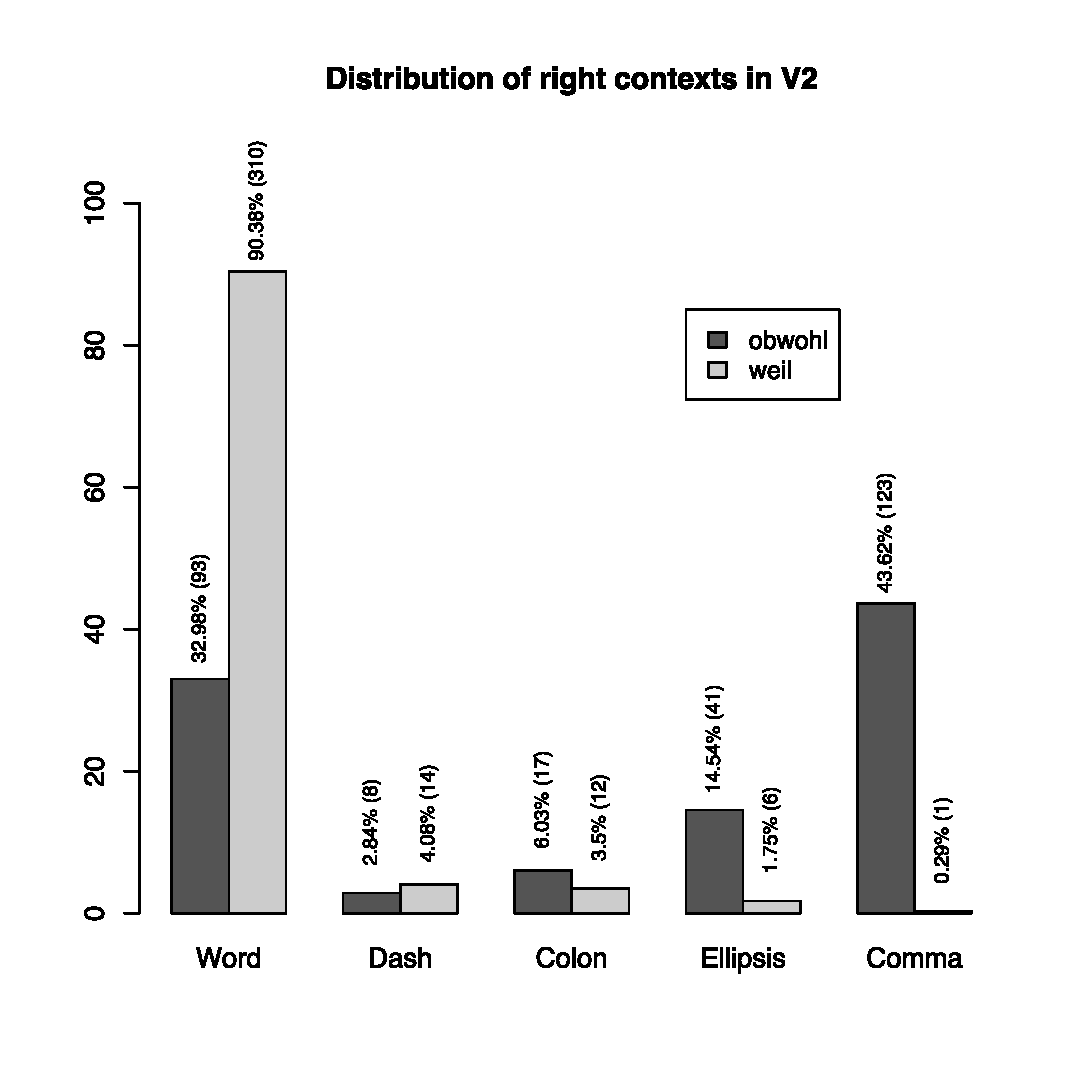
\includegraphics[height=0.9\textheight]{v2_right}
\end{frame}

\begin{frame}
	{Interpretation}
	\centering
	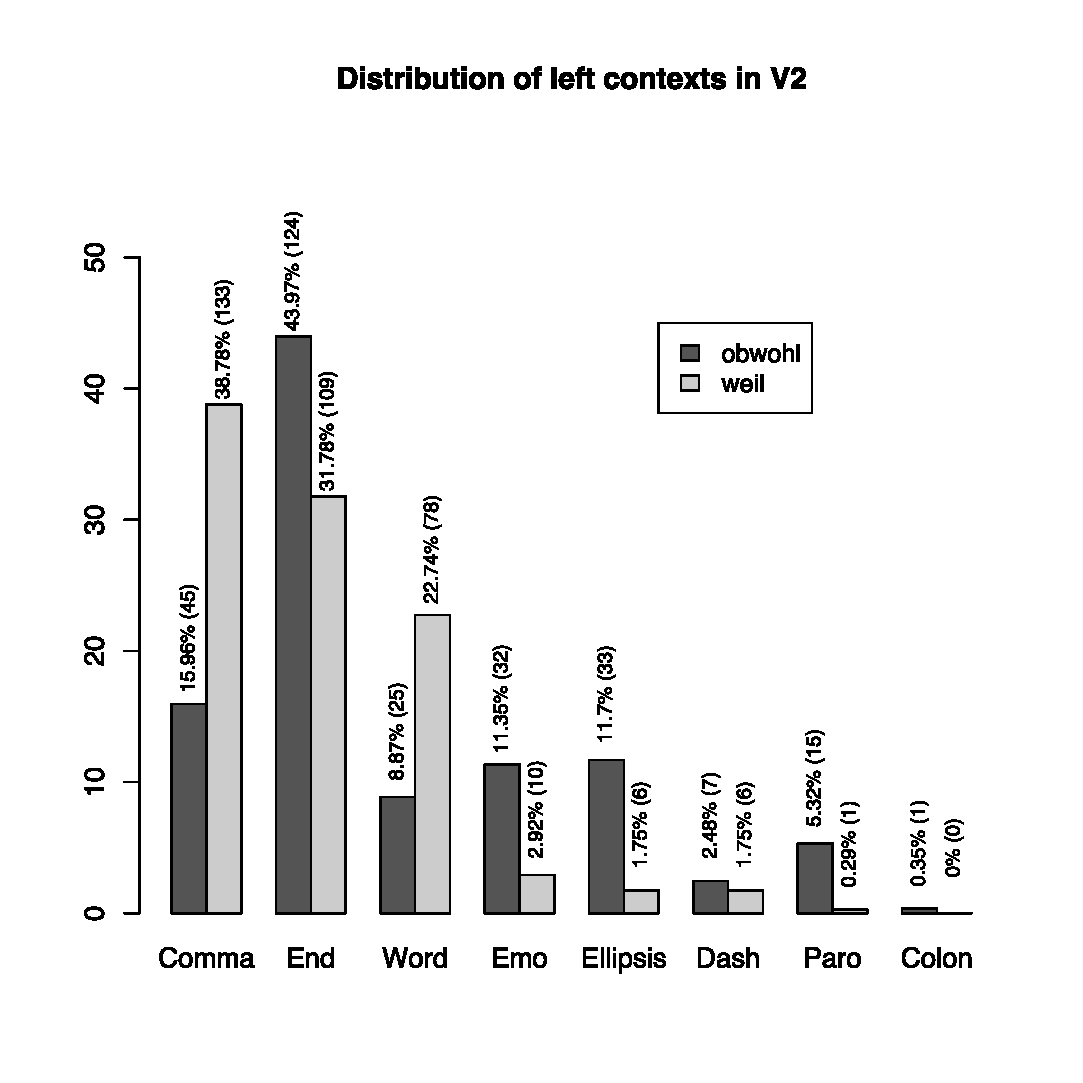
\includegraphics[height=0.9\textheight]{v2_left}
\end{frame}


%\subsection{Schwache Substantive}

\begin{frame}
	{Schäfer (2016, erscheint in CLLT)}
	\begin{itemize}
	  \item \textit{einen Linguisten} vs.\ \textit{einen Linguist}
	  \item schwache Substantive: absolute Exoten\\im nominalen Flexionssystem
	  \item Köpcke (1995): 2 oder mehr Prototypen\\sichern Erhalt der Flexionsklasse
	  
	  \vspace{0.5cm}
	  
	  \item \alert{Idee: Die Alternation sollte bei weniger prototypischen\\schwachen Substantiven häufiger auftreten.}
	  
	  \vspace{0.5cm}
	  
	  \item DECOW-Studie mit ca.\ 500 Lemmata\\und \alert{500,000 Belegen}
	\end{itemize}
\end{frame}

\begin{frame}
	{Die Alternation als seltenes Ereignis}
	\centering
	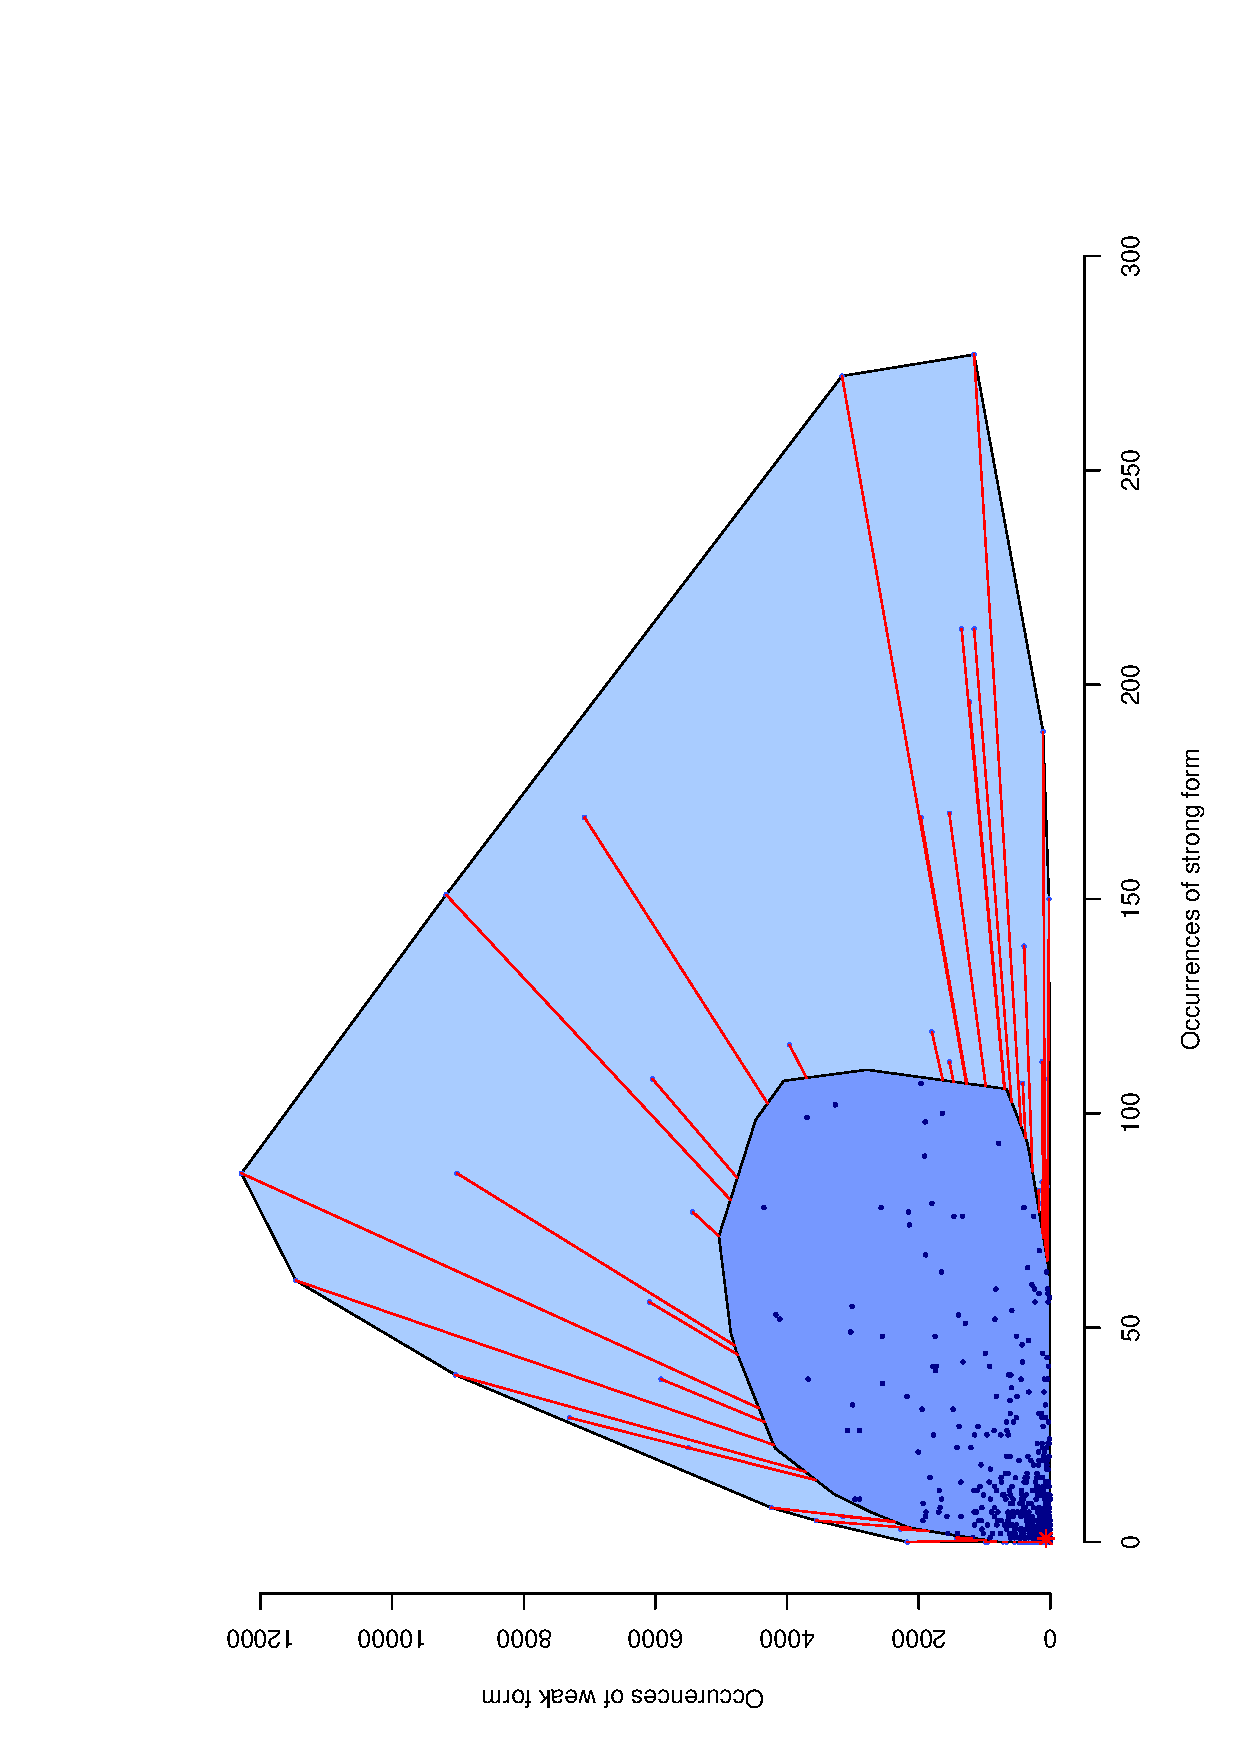
\includegraphics[height=0.95\textheight,angle=270]{bag}
\end{frame}

\begin{frame}
	{Köpckes (1995) Prototypen}
	\centering
	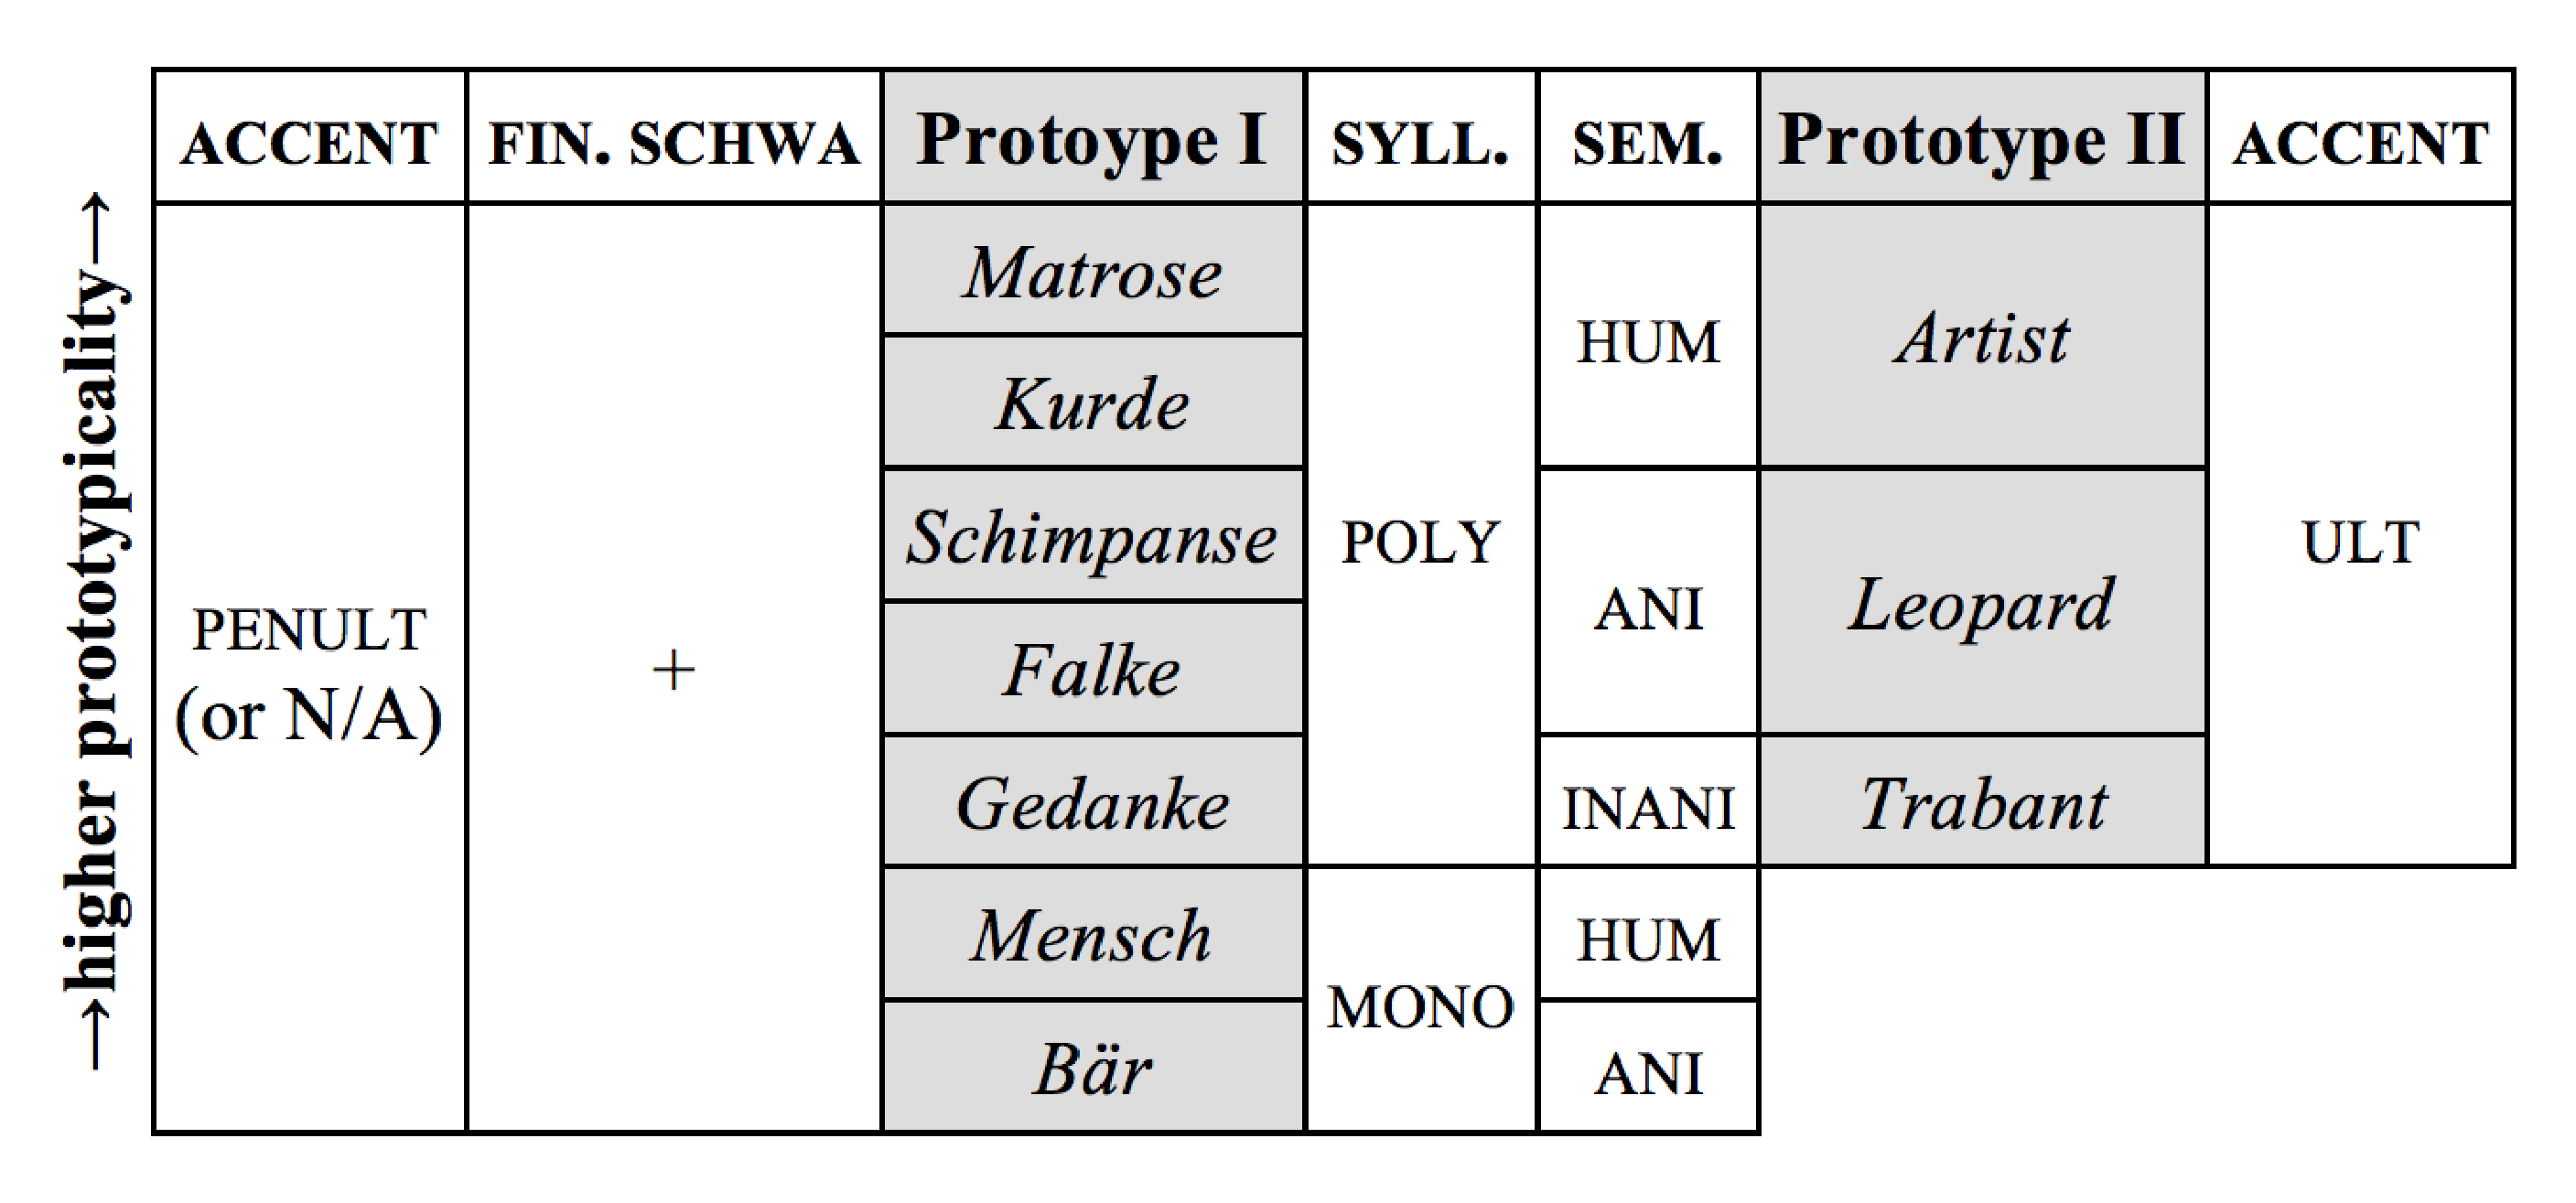
\includegraphics[height=0.6\textheight]{koepcke}
\end{frame}

\begin{frame}
	{... kontrollieren die Alternationsstärke!}
	\centering
	\includegraphics[height=0.6\textheight]{schaefer}\\
	\vspace{0.5cm}
	summierte Chancenverhältnisse für die (Sub-)Prototypen\\
	die Wörter sind nur Beispiele!
\end{frame}


%\subsection{Maßangaben und Variation Mining}

\newcommand{\Gen}{\ensuremath{_{\mathsf{Gen}}}}
\newcommand{\Acc}{\ensuremath{_{\mathsf{Acc}}}}


\begin{frame}
	{Schäfer (wird 2016 eingereicht)}
	\scalebox{0.85}{\begin{minipage}{1.2\textwidth}
	\begin{exe}
		\ex\gll Wir trinken eine Flasche [des {Weines]\Gen} {\slash} *[den Wein]\Acc.\\
			we drink a bottle [the wine]{\Gen} {\slash} \hspaceThis{*}[the wine]\\
			\glt {\it We drink a bottle of the wine.}
		\ex\gll Wir trinken eine Flasche {*Weines\Gen} {\slash} Wein\Acc.\\
			we drink a bottle \hspaceThis{*}wine {\slash} wine\\
			\glt {\it We drink a bottle of wine.}
		\ex\gll Wir trinken eine Flasche [leckeren {Weines]\Gen} {\slash} [leckeren Wein]\Acc.\\
			we drink a bottle tasty wine / tasty wine\\
			\glt {\it We drink a bottle of tasty wine.}
	\end{exe}
	\end{minipage}}
\end{frame}

\begin{frame}
	{German measure NPs}
	\begin{itemize}
		\item measure phrases in the broad sense
		\item {$[N_{measure}\ Det\ (AP)\ N_{kind}]$}: case of $N_{kind}$ always genitive
		\item {$[N_{measure}\ N_{kind}]$}: always case identity
		\item {$[N_{measure}\ AP\ N_{kind}]$}: genitive or case identity 
	\end{itemize}
\end{frame}

%\begin{frame}
%	{Case syncretism in the feminine}
%	\begin{itemize}
%		\item feminine NPs: syncretisms of nom\slash acc and dat\slash gen
%		\item nom\slash acc: \textit{(eine\slash die) frische Sahne}
%		\item dat\slash gen: \textit{(einer\slash der) frischen Sahne\slash frischer Sahne}
%		\item decision not between case-identity and genitive construction\\
%			but case-identity and obliqueness-drop construction
%	\end{itemize}
%\end{frame}
%
%\begin{frame}
%	{Descriptive gap}
%	\begin{itemize}
%		\item descriptions in grammars\\(e.g., Eisenberg 2013, Engel 2009)
%		\item genitive construction: \textit{partitive genitive}
%		\item case-identity construction: \textit{narrow apposition}
%	\end{itemize}
%\end{frame}

%\begin{frame}
%	{Unambiguous structures (semi-hypothetical account)}
%	\centering
%	\scalebox{0.8}{\begin{minipage}{0.5\textwidth}\centering
%	\begin{forest}
%		[DP [D[eine]] [NP [N[Flasche]] [NP[Wein]] ]] ]]
%	\end{forest}
%	\end{minipage}}
%	\scalebox{0.8}{\begin{minipage}{0.5\textwidth}\centering
%	\begin{forest}
%		[DP [D[eine]] [NP [N[Flasche]] [DP [D[des]] [NP [AP[guten]] [N[Weines]] ] ]]]
%	\end{forest}
%	\end{minipage}}
%\end{frame}
%
%\begin{frame}
%	{Ambiguous structures (semi-hypothetical account)}
%	\centering
%	\scalebox{0.8}{\begin{minipage}{0.5\textwidth}\centering
%	\begin{forest}
%		[DP [D[eine]] [NP [N[Flasche]] [NP [AP[guter]] [N[Wein]]] ]] ]]
%	\end{forest}
%	\end{minipage}}
%	\scalebox{0.8}{\begin{minipage}{0.5\textwidth}\centering
%	\begin{forest}
%		[DP [D[eine]] [NP [N[Flasche]] [DP [D[guten]] [NP [Weines]] ] ]]
%	\end{forest}
%	\end{minipage}}
%\end{frame}
%
%\begin{frame}
%	{Sense and syntacticality}
%	\begin{itemize}
%		\item configurational approaches like that in\\Bhatt (1990), Gallmann \& Lindauer (1994), etc.
%		\item interestingly: often, one alternative considered \textit{ungrammatical}
%		\item sometimes additional \textit{QP} level
%		\item Gallmann (1990): single structure for both constructions
%		\item long-winded \textit{proofs}, that measure noun is the higher head (Löbel 1990, Bhatt 1990)
%		\item ... trivial, because of simple agreement facts
%	\end{itemize}
%\end{frame}
%
%\begin{frame}
%	{"The rich literature on partitives"}
%	\footnotesize
%	Partitives\slash Pseudo-partitives\slash Partitive Constraint
%	\begin{itemize}
%		\item partitives: embedded NP is definite = \textit{Partitive Constraint}\\
%			(e.\,g., Jackendoff 1977, Ladusaw 1982, Selkrik 1977, Vos 1999)
%		\item not even true for German \textit{partitive genitive} construction
%		\item German constructions: pseudo-partitives, if anything
%		\item Anttila \& Fong (2001): refined PC (\textit{quantificational determinacy})\\
%			plus some allegedly universal syntactic constraints (\textit{syntactic OCP})\\
%			to account for a highly non-similar alternation in Finnish
%		\item Eschenbach (1991) on German measure constructions:\\
%			more refined semantics, again irrelevant for our purposes
%	\end{itemize}
%\end{frame}
%
%\begin{frame}
%	{To sum up\ldots}
%	\begin{itemize}
%		\item no relevant insight from configurational approaches
%		\item no help from semantics of measurement\slash partitivity
%		\vspace{0.5cm}
%		\item \alert{no strong theoretical hypotheses\\about what drives the alternation}
%	\end{itemize}
%\end{frame}
%
%\begin{frame}
%	{Hentschel (2003)}
%	\begin{itemize}
%		\item questionnaire study
%		\item descriptive, no theoretical approach
%		\item results:
%			\begin{enumerate}
%				\item overall tendency for case identity
%				\item genitive preferred with plural nouns
%				\item verb-governed accusative: identity preferred
%			\end{enumerate}
%	\end{itemize}
%\end{frame}
%
%\subsection{Corpus study}
%
%\subsubsection{General research paradigm}

\begin{frame}
	{Alternations}
	\begin{itemize}
		\item \textit{alternations}
			\begin{itemize}
				\item competing constructions, given contexts\slash lexical choices
				\item competing items, given constructions
			\end{itemize}
		\item established paradigm: alternations as neither fully random\\
			nor controlled by discrete (even single) factors
		\item cognitively motivated: item-specific and\slash or context-specific\\
			influences on the probabilities of choices
		\item e.g., Gries (2003), Gries \& Stefanowitsch (2003 et alibi), Bresnan et al. (2007), Arppe (2009), Nesset \& Janda (2010), Divjak \& Arppe (2013), Bart \& Kapatsinski (2014 aop)
	\end{itemize}
\end{frame}

%\subsubsection{Sample(s)}
%
%\begin{frame}
%	{2012 sample}
%	\begin{itemize}
%		\item DEWAC (Baroni et al. 2009)
%		\item 30 intuitively chosen mass nouns (10 per gender)
%		\item only mass nouns (singular) 
%		\item search for sequences [N A specific-mass-noun]
%		\item filter by hand, annotate for case of measure noun
%		\item 687 masculine, 1007 neuter, 421 feminine NPs
%		\item because of low frequency of genitives,\\samples were stratified: 50\% for each level of response
%	\end{itemize}
%\end{frame}
%
%\begin{frame}
%	{2015 sample}
%	\begin{itemize}
%		\item corpus: DECOW14A (Schäfer \& Bildhauer 2012\ldots), 20 GT
%		\item again: only mass nouns (singular) 
%		\item bootstrap process:
%			\begin{enumerate}
%				\item manually extract 100 most frequent mass nouns
%				\item search pattern [N D A* N mass-noun]
%				\item manually extract the 20 most frequent measure nouns\\for each mass noun
%				\item query combinations [measure-noun A mass-noun]
%			\end{enumerate}
%		\item final sample (after filtering\slash cleaning):\\
%			4172 masculine\slash neuter, 1114 feminine
%		\item as opposed to DEWAC sample, DECOW14A sample covers\\
%			all frequent combinations of measure and mass nouns
%	\end{itemize}
%\end{frame}

%\subsubsection{GLMs for DEWAC dataset}

%\begin{frame}
%	{DEWAC: Masculine\slash Neuter}
%  \centering
%  \scalebox{0.8}{
%  \begin{tabular}{lrrcp{1cm}rrc}
%    \multicolumn{1}{c}{} & \multicolumn{3}{c}{\textbf{Masculine}} && \multicolumn{3}{c}{\textbf{Neuter}} \\
%    \hline
%    \textbf{Regressor} & \textbf{Coeff.} & \textbf{OR} & \textbf{Sign.} && \textbf{Coeff.} & \textbf{OR} & \textbf{Sign.} \\
%    \hline
%    \hline
%    \textsc{(Intercept)} & -1.95 & 0.14 & *** && -3.37 &  0.03 & *** \\
%    \textsc{MeasurecaseNom}   &  0.31 & 1.37 &   . && -0.01 &  0.99 &     \\
%    \textsc{MeasurecaseDat}   &  0.31 & 1.37 &   * &&  0.92 &  2.50 & *** \\
%    \textsc{Measurenoundefinite1}      &  1.47 & 4.36 & *** &&  2.67 & 14.48 & *** \\
%    \textsc{Kindfreq}    &  0.03 & 1.03 & *** &&  0.82 &  2.27 & *** \\
%    \textsc{Measureabbreviated1}     & -3.05 & 0.05 & *** && -4.92 &  0.01 & *** \\
%    \hline
%  \end{tabular}}\\
%  \vspace{0.5cm}
%	\footnotesize predicting \textsc{genitive construction}; model selection by step-down; internal and 10-fold cross validation accuracy is $78.01\%$ for masculine, $75.65\%$ for neuter; Nagelkerke's $R^2=0.22$ for masculine, $R^2=0.29$ for neuter; dispersion $\hat\phi=0.99$ for masculine, $\hat\phi=0.95$ for neuter
%\end{frame}
%
%\begin{frame}
%	{DEWAC: Feminine}
%  \centering
%  \scalebox{0.75}{
%  \begin{tabular}{lrrc}
%    \hline
%    \textbf{Regressor} & \textbf{Coeff.} & \textbf{OR} & \textbf{Sign.} \\
%    \hline
%    \hline
%    \textsc{(Intercept)} &  4.08 & 59.41 & *** \\
%    \textsc{MeasurecaseAcc}   & -0.16 &  0.85 &     \\
%    \textsc{MeasurecaseDat}      & -2.33 &  0.10 &   * \\
%    \textsc{Kindfreq}    & -2.00 &  0.14 & *** \\
%    \textsc{Measureabbreviated1}     &  3.65 & 38.38 & *** \\
%    \hline
%  \end{tabular}}\\
%  \vspace{0.5cm}
%	\footnotesize predicting \textsc{case agreement}; model selection by step-down; internal and 10-fold cross validation accuracy is $80.71\%$; Nagelkerke's $R^2=0.62$, dispersion is $\hat{\phi}=0.87$
%\end{frame}

%\subsubsection{GLMs from DECOW14 dataset}

\begin{frame}
	{DECOW14A model summary: masculine and neuter}
	\centering
	\scalebox{0.5}{
	\begin{tabular}{lrrrrrc}
	\hline
                   &  Estimate& OR & Std. Error& z value& Pr(>|z|)&    \\
	\hline
	\hline
		(Intercept)        & -12.36736& 0.0000 &  0.99790& -12.393&  < 2e-16& ***\\
		MeasurecaseAcc     &   0.03406& 1.0346 &  0.11721&   0.291& 0.771352&    \\
		MeasurecaseDat     &   0.49126& 1.6343 &  0.13569&   3.621& 0.000294& ***\\
		Kindlength         &   0.61327& 1.8464 &  0.03434&  17.859&  < 2e-16& ***\\
		KindfinalclassFric &  -0.04110& 0.9597 &  0.23217&  -0.177& 0.859490&    \\
		KindfinalclassRvo  &  -0.07985& 0.9232 &  0.22898&  -0.349& 0.727293&    \\
		KindfinalclassPlos &   0.52423& 1.6891 &  0.22652&   2.314& 0.020651& *  \\
		KindfinalclassLiq  &   0.85280& 2.3461 &  0.24504&   3.480& 0.000501& ***\\
		KindfinalclassNas  &   0.77421& 2.1688 &  0.24397&   3.173& 0.001507& ** \\
		Kindedible0        &   0.75699& 2.1318 &  0.12396&   6.106& 1.02e-09& ***\\
		Kindfreq           &   1.92525& 6.8568 &  0.16232&  11.861&  < 2e-16& ***\\
		MeasuregenderMasc  &   0.01090& 1.0109 &  0.15411&   0.071& 0.943634&    \\
		MeasuregenderFem   &   0.35432& 1.4252 &  0.13988&   2.533& 0.011308& *  \\
		MeasurenumberPl    &   0.86330& 2.3709 &  0.14906&   5.792& 6.97e-09& ***\\
		Measureabbreviated0&   1.53688& 4.6500 &  0.32499&   4.729& 2.26e-06& ***\\
		Measurelength      &  -0.12810& 0.8797 &  0.03397&  -3.771& 0.000163& ***\\
		Measurefreq        &  -0.58232& 0.5585 &  0.09269&  -6.282& 3.33e-10& ***\\
		Minus1posP         &   1.18411& 3.2677 &  0.21357&   5.544& 2.95e-08& ***\\
		Minus1posN         &   0.23117& 1.2600 &  0.26573&   0.870& 0.384328&    \\
		Minus1posA         &   1.86418& 6.4506 &  0.14891&  12.518&  < 2e-16& ***\\
		Minus1posO         &   2.04921& 7.7617 &  0.38346&   5.344& 9.09e-08& ***\\
		Genitives          &  -0.32547& 0.7221 &  0.02732& -11.913&  < 2e-16& ***\\
		Badness            &  -0.09064& 0.9133 &  0.02613&  -3.468& 0.000524& ***\\
	\hline
	\end{tabular}
	}
\end{frame}
%
%\begin{frame}
%	{DECOW14A model evaluation: masculine and neuter}
%	\centering
%	\begin{tabular}{llll}
%		Sample size & n &=&  4172 \\
%		Nagelkerke  & $R^2$ &=&  0.431 \\
%		Dispersion  & $\phi$ &=&  0.894 \\
%		LR Test     & LR &=&  1257.841 (df =  22, p =  0)\\
%		10-CV       & $\Delta$ &=&  0.09994593 \\
%		Baseline    & $\epsilon$ &=&  0.1744966 \\
%		Reduction   & pre &=&  0.4272329 \\
%	\end{tabular}
%\end{frame}
%
%\begin{frame}
%	{DECOW14A variance inflation: masculine and neuter}
%	Dropped for extreme collinearity:
%	\vspace{1cm}
%	\begin{enumerate}
%		\item semantics of mass noun: \textit{consistency}
%		\item semantics of mass noun: \textit{origin}
%		\item semantics of mass noun: \textit{artefact}
%		\item semantics of measure noun: \textit{semantic class}
%	\end{enumerate}
%\end{frame}
%
%\begin{frame}
%	{DECOW14A variance inflation: masculine and neuter}
%	\centering
%	\scalebox{0.8}{
%	\begin{tabular}{lrrr}
%	\hline
%		                  &     $GVIF$& $Df$& $GVIF^(1/(2*Df))$\\
%	\hline
%	\hline
%		Measurecase       & 1.068292&  2&        1.016652\\
%		Kindlength        & 1.609944&  1&        1.268836\\
%		Kindfinalclass    & 2.250817&  5&        1.084511\\
%		Kindedible        & 1.465327&  1&        1.210507\\
%		Kindfreq          & 1.338470&  1&        1.156923\\
%		Measuregender     & 1.596935&  2&        1.124144\\
%		Measurenumber     & 1.626972&  1&        1.275528\\
%		Measureabbreviated& 1.355320&  1&        1.164182\\
%		Measurelength     & 1.974751&  1&        1.405258\\
%		Measurefreq       & 1.740086&  1&        1.319123\\
%		Minus1pos         & 1.787250&  4&        1.075284\\
%		Genitives         & 1.121494&  1&        1.059006\\
%		Badness           & 1.039426&  1&        1.019523\\
%	\hline
%	\end{tabular}
%	}
%\end{frame}
%
%

\begin{frame}
	{DECOW14A model summary: feminine}
	\centering
	\scalebox{0.7}{
	\begin{tabular}{lrrrrrc}
	\hline
                   &  Estimate& OR &Std. Error& z value& Pr(>|z|)&    \\
	\hline
	\hline
		(Intercept)      & -3.26446 &  0.0382&  1.00948&  -3.234&  0.00122& ** \\
		Kindedible0      &  1.38772 &  4.0057&  0.18586&   7.467& 8.23e-14& ***\\
		MeasuregenderMasc&  0.98742 &  2.6842&  0.22957&   4.301& 1.70e-05& ***\\
		MeasuregenderFem &  0.46838 &  1.5973&  0.21722&   2.156&  0.03107& *  \\
		MeasurenumberPl  &  1.50316 &  4.4958&  0.29577&   5.082& 3.73e-07& ***\\
		Measurelength    & -0.30782 &  0.7350&  0.06044&  -5.093& 3.52e-07& ***\\
		Measurefreq      & -0.46196 &  0.6300&  0.15652&  -2.951&  0.00316& ** \\
		Minus1posP       &  1.90609 &  6.7267&  0.39414&   4.836& 1.32e-06& ***\\
		Minus1posN       &  0.68847 &  1.9906&  0.59486&   1.157&  0.24712&    \\
		Minus1posA       &  3.06176 & 21.3650&  0.28243&  10.841&  < 2e-16& ***\\
		Minus1posO       &  3.09771 & 22.1472&  0.55616&   5.570& 2.55e-08& ***\\
		Matchlength      &  0.17986 &  1.1970&  0.02229&   8.069& 7.09e-16& ***\\
		Genitives        & -0.29002 &  0.7482&  0.04288&  -6.764& 1.34e-11& ***\\
	\hline
	\end{tabular}
	}
\end{frame}
%
%\begin{frame}
%	{DECOW14A model evaluation: feminine}
%	\centering
%	\begin{tabular}{llll}
%		Sample size&  n& = & 1114 \\
%		Nagelkerke & $R^2$& = & 0.491 \\
%		Dispersion &  $\phi$& = & 1.053 \\
%		LR Test    & LR& = & 505.8554 (df =  12,    p =  0)\\
%		10-CV      &  $\Delta$& = & 0.151722 \\
%		Baseline   &  $\epsilon$& = & 0.4147217 \\
%		Reduction  &pre& = & 0.6341595 \\
%	\end{tabular}
%\end{frame}
%
%\begin{frame}
%	{DECOW14A variance inflation: feminine}
%	\centering
%	\scalebox{0.8}{
%	\begin{tabular}{lrrr}
%	\hline
%		                  &     $GVIF$& $Df$& $GVIF^(1/(2*Df))$\\
%	\hline
%	\hline
%		Kindedible   & 1.209434 & 1 &       1.099743\\
%		Measuregender& 1.780486 & 2 &       1.155140\\
%		Measurenumber& 1.657590 & 1 &       1.287474\\
%		Measurelength& 2.279081 & 1 &       1.509663\\
%		Measurefreq  & 2.120574 & 1 &       1.456219\\
%		Minus1pos    & 1.766196 & 4 &       1.073692\\
%		Matchlength  & 1.484503 & 1 &       1.218402\\
%		Genitives    & 1.101343 & 1 &       1.049449\\
%
%	\hline
%	\end{tabular}
%	}
%\end{frame}
%
%\begin{frame}
%	{A note on random effects}
%	\begin{itemize}
%		\item the mass noun lemma as a random effect was significant\\for DEWAC data
%		\item fixed effects \alert{not} masked by RE
%		\item slight increase in accuracy and $R^2$
%		\item for DECOW data: problems with model estimation\slash evaluation
%		\item \textit{speaker}, \textit{genre} not available (no meta data)
%		\item current work on COW might improve that
%	\end{itemize}
%\end{frame}

%\subsubsection{Multimodel approach for DECOW14 dataset}

\begin{frame}
	{Multimodel inference}
	\begin{itemize}
		\item some of problems with stepwise regression:
			\begin{enumerate}
				\item likely incorrect fiction of availability of a best model\\
					approximating absolute truth
				\item spurious significances\\
					\alert{especially with large samples}
				\item \textit{data dredging} without strong\\
					theoretically motivated hypotheses
			\end{enumerate}
		\item solution: consider some or even many good models
		\item model weighting by information criterion like AIC(c), BIC(c)
		\item find and average \textit{important} coefficients across models
		\item Burnham \& Anderson (2002), in linguistics:\\Kuperman \& Bresnan (2012), Bart \& Kapatsinski (2014 aop)
	\end{itemize}
\end{frame}

\begin{frame}
	{Under the circumstances...}
	\begin{itemize}
		\item We don't have strong hypotheses.
		\item But we do have large samples.
		\item Sounds like a case for MMI.
	\end{itemize}
\end{frame}

\begin{frame}
	{Multimodel averaging: masculine and neuter}
	\centering
	\includegraphics[height=0.8\textheight]{mn_aic_multi}\\
	\tiny genetic algorithm, search through full model space without interactions and random effects
\end{frame}

\begin{frame}
	{Multimodel averaging: feminine}
	\centering
	\includegraphics[height=0.8\textheight]{fem_aic_multi}\\
	\tiny genetic algorithm, search through full model space without interactions and random effects
\end{frame}

%\subsubsection{AIC and BIC}
%
%\begin{frame}
%	{Which IC to use: masculine and neuter}
%	\centering
%	\includegraphics[width=0.5\textwidth]{mn_aic_multi}~\includegraphics[width=0.51\textwidth]{mn_bic_multi}
%\end{frame}
%
%\begin{frame}
%	{Which IC to use: feminine}
%	\centering
%	\includegraphics[width=0.5\textwidth]{fem_aic_multi}~\includegraphics[width=0.51\textwidth]{fem_bic_multi}
%\end{frame}
%
%\begin{frame}
%	{Source of difference between AIC and BIC for masculine}
%	\centering
%	\includegraphics[width=0.5\textwidth]{bic_vs_aic_mn}~\includegraphics[width=0.5\textwidth]{bic_vs_aic_fem}
%\end{frame}
%

%\subsection{(Preliminary) conclusions and the future}

\begin{frame}
	{Comparison of results}
	\centering
	\scalebox{0.4}{
	\begin{tabular}{lp{0.2cm}cccccp{0.2cm}cccc}
		&& \multicolumn{5}{c}{masc\slash neut} && \multicolumn{4}{c}{fem} \\
		\cline{3-7}\cline{9-12}
		regressor && DEWAC m & DEWAC n & COW & COW AIC & COW BIC && DEWAC & COW & COW AIC & COW BIC \\
		\hline
		\hline
		Badness             &&     &     &     & $-$ & $-$ &&     &     &     &   \\
		\hline
		\alert<2->{Genitives}           &&     &     &     & $-$ & $-$ &&     & $-$ & $-$ & $-$ \\
		\hline
		Kindedible0         &&     &     & $+$ & $+$ & $+$ &&     & $+$ & $+$ & $+$ \\
		\alert<2->{Kindedible1}         &&     &     & $-$ & $-$ & $-$ &&     & $-$ & $-$ & $-$ \\
		\hline
		KindfinalclassFric  &&     &     &     & $-$ &     &&     &     &     &   \\
		KindfinalclassLiq   &&     &     & $+$ & $+$ &     &&     &     &     &   \\
		KindfinalclassNas   &&     &     & $+$ & $+$ &     &&     &     &     &   \\
		KindfinalclassPlos  &&     &     & $+$ & $+$ &     &&     &     &     &   \\
		KindfinalclassRvo   &&     &     &     & $-$ &     &&     &     &     &   \\
		KindfinalclassV     &&     &     & $-$ & $-$ &     &&     &     &     &   \\
		\hline
		\alert<2->{Kindfreq}            && $+$ & $+$ & $+$ & $+$ & $+$ && $+$ &     &     &   \\
		\hline
		Kindlength          &&     &     & $+$ & $+$ & $+$ &&     &     &     &   \\
		\hline
		Matchlength         &&     &     &     &     &     &&     & $+$ & $+$ & $+$ \\
		\hline
		Measureabbreviated0 && $+$ & $+$ & $+$ & $+$ & $+$ && $+$ &     &     &   \\
		\alert<2->{Measureabbreviated1} && $-$ & $-$ & $-$ & $-$ & $-$ && $-$ &     &     &   \\
		\hline
		MeasurecaseAcc      && $-$ & $-$ & $-$ &($+$)&     && $-$ &     &     &   \\
		MeasurecaseNom      && $-$ & $-$ & $-$ & $-$ &     && $-$ &     &     &   \\
		\alert<2->{MeasurecaseDat}      && $+$ & $+$ & $+$ & $+$ &     && $+$ &     &     &   \\
		\hline
		\alert<2->{Measurefreq}         &&     &     & $-$ & $-$ & $-$ &&     &     & $-$ & $-$ \\
		\hline
		MeasuregenderFem    &&     &     & $+$ & $+$ &     &&     & $+$ & $+$ & $+$ \\
		MeasuregenderMasc   &&     &     & $-$ &($+$)&     &&     & $+$ & $+$ & $+$ \\
		MeasuregenderNeut   &&     &     & $-$ & $-$ &     &&     & $-$ & $-$ & $-$ \\
		\hline
		\alert<2->{Measurelength}       &&     &     & $-$ & $-$ & $-$ &&     & $-$ & $-$ & $-$ \\
		\hline
		MeasurenumberSg     &&     &     & $-$ & $-$ & $-$ &&     & $-$ & $-$ & $-$ \\
		\alert<2->{MeasurenumberPl}     &&     &     & $+$ & $+$ & $+$ &&     & $+$ & $+$ & $+$ \\
		\hline
		Minus1posA          &&     &     & $+$ & $+$ & $+$ &&     & $+$ & $+$ & $+$ \\
		\alert<2->{Minus1posC}          &&     &     & $-$ & $-$ & $-$ &&     & $-$ & $-$ & $-$ \\
		Minus1posN          &&     &     &     & $+$ & $+$ &&     &     & $+$ & $+$ \\
		Minus1posO          &&     &     & $+$ & $+$ & $+$ &&     & $+$ & $+$ & $+$ \\
		Minus1posP          &&     &     & $+$ & $+$ & $+$ &&     & $+$ & $+$ & $+$ \\
		\hline
	\end{tabular}
	}
\end{frame}

%
%
\section{Zugriff auf COW}


\begin{frame}
  {Everybody}
  \begin{itemize}
    \item n-grams ($n=1..5$)
    \item DE/EN dependency bigrams 
    \item frequency lists
    \item link data
    \item in the future: COCOA
    \item \url{http://hpsg.fu-berlin.de/cow/}
  \end{itemize}
\end{frame}

\begin{frame}
  {Researchers\slash academia: \url{https://webcorpora.org/}}
  \centering
  \includegraphics[height=0.5\textheight]{./graphics/colistart}  
  \begin{itemize}
    \item Colibri²: simple and fast (shuffle corpora)
    \item NoSketchEngine: powerful, fast, full corpora,\\
      but export restrictions
    \item download of shuffle corpora (XML)
    \item RStudio Server (ask \& pay)
  \end{itemize}
\end{frame}

%\begin{frame}
%  {FU-intern und Kooperationspartner}
%  \begin{itemize}
%    \item NoSketch Engine: \alert{volle Korpora}
%    \item Vorteil ggü.\ CWB-basierten Lösungen: Geschwindigkeit, Korpusgrößen
%    \item \ldots Demo im Anschluss \ldots
%    \item alternativ: CQP-Konsole
%  \end{itemize}
%\end{frame}



% --------------- REFS + APPENDIX

\begin{frame}
  {Zusammenfassung und Ausblick}
  Wir liefern\dots\\
  \begin{itemize}
    \item \alert{große Webkorpora}
    \item rechtssichere \alert{Umgehung des Urheberrechts}
    \item \alert{Nachverarbeitung} auf dem Stand der Technik
    \item bald \alert{verzerrungsfreie Referenzkorpora}
    \item Grundlagenforschung zur \alert{Webkorpuszusammensetzung}
    \item \alert{Dokumentklassifikation} ohne konzeptuellen Ballast\\
      zugunsten der Zuverlässigkeit bzw.\ der Operationalisierung
  \end{itemize}
\end{frame}

%\begin{frame}[allowframebreaks]
%  {References}
%  \def\newblock{\hskip .11em plus .33em minus .07em}
%  \tiny
%  \bibliographystyle{abbrvnat} 
%  \bibliography{cow,felix}
%\end{frame}

\makeatletter
\setcounter{lastpagemainpart}{\the\c@framenumber}
\makeatother

%\appendix
%
%\section{Appendix}

\mode<beamer>{\setcounter{framenumber}{\thelastpagemainpart}}

\end{document}
 
